\documentclass[]{spie}  %>>> use for US letter paper

\usepackage{graphicx}
\usepackage{subfig}
\usepackage{amsmath}
\usepackage{amssymb}
\usepackage{hyperref}
\usepackage{float}
\usepackage{multirow}

\title{Texture Mapping 3D Models of Indoor Environments with Noisy Camera Poses} 

\author{Peter Cheng
\skiplinehalf
University of California, Berkeley\\
}

\begin{document}
\maketitle

%%%%%%%%%%%%%%%%%%%%%%%%%%%%%%%%%%%%%%%%%%%%%%%%%%%%%%%%%%%%% 
\begin{abstract}
  Automated 3D modeling of building interiors is used in applications
  such as virtual reality and environment mapping. Texturing these
  models allows for photo-realistic visualizations of the data
  collected by such modeling systems. While data acquisition times for
  mobile mapping systems are considerably shorter than for static
  ones, their recovered camera poses often suffer from inaccuracies,
  resulting in visible discontinuities when successive images are
  projected onto a surface for texturing. We present a method for
  texture mapping models of indoor environments that starts by
  selecting images whose camera poses are well-aligned in two
  dimensions. We then align images to geometry as well as to each
  other, producing visually consistent textures even in the presence
  of inaccurate surface geometry and noisy camera poses. Images are
  then composited into a final texture mosaic and projected onto
  surface geometry for visualization. The effectiveness of the
  proposed method is demonstrated on a number of different indoor
  environments.
\end{abstract}

% >>>> Include a list of keywords after the abstract

\keywords{Texture Mapping, Reconstruction, Image Stitching, Mosaicing}

%%%%%%%%%%%%%%%%%%%%%%%%%%%%%%%%%%%%%%%%%%%%%%%%%%%%%%%%%%%%%
\section{Introduction}
\label{sec:introduction} % \label{} allows reference to this section
Three-dimensional modeling of indoor environments has a variety of
applications such as training and simulation for disaster management,
virtual heritage conservation, and mapping of hazardous sites. Manual
construction of these digital models can be time consuming, and
consequently automated 3D site modeling has garnered much interest in
recent years.

The first step in automated 3D modeling is the physical scanning of
the environment's geometry. An indoor modeling system must be able to
recover its pose within an environment while simultaneously
reconstructing the 3D structure of the environment itself
\cite{chen2010indoor, hz, kua2012loopclosure, liu2010indoor}. This is
known as the simultaneous localization and mapping (SLAM) problem, and
is generally solved by taking readings from laser range scanners,
cameras, and inertial measurement units (IMUs) at multiple locations
within the environment. Mounting such devices on a platform carried by
an ambulatory human provides unique advantages over static or
vehicular-based systems on wheels in terms of agility and portability,
but can also result in larger localization error
\cite{liu2010indoor}. As a result, common methods for texture mapping
generally produce poor results. In this thesis, we present an approach
to texture mapping 3D models of indoor environments in the presence of
uncertainty and noise in camera poses. In particular, we consider data
obtained from a human-operated backpack system, detailed in Section
\ref{sec:dataAcquisition}.


\begin{figure}
  \centering
  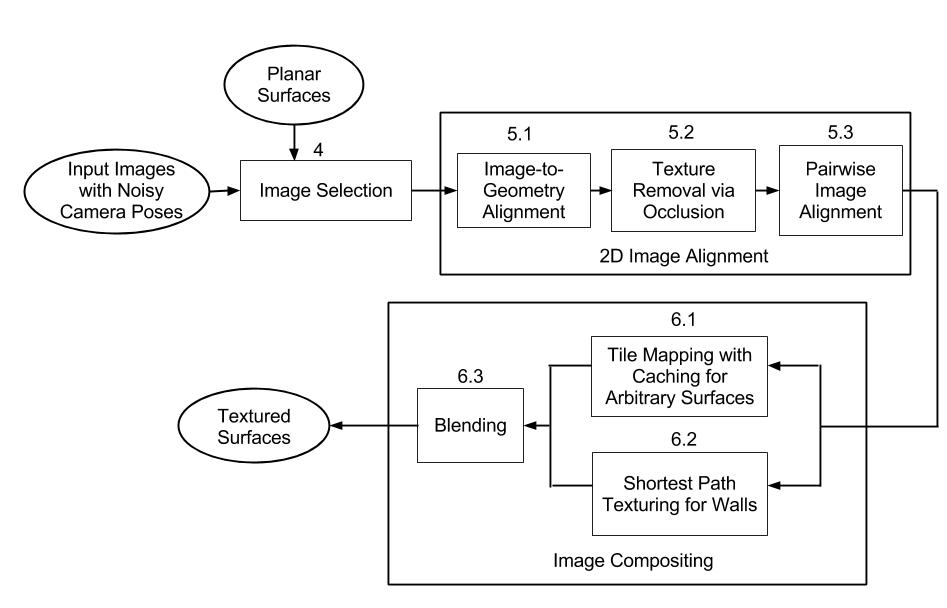
\includegraphics[width=6in]{flowchart.jpg}
  \caption{The proposed texture mapping procedure\\}
  \label{fig:flowchart}
\end{figure}


The overall block diagram for the proposed texture mapping procedure
is shown in Figure \ref{fig:flowchart}, where the number attached to
each box indicates the section in which the concept in the box is
explained in this thesis. First, the geometry of an environment is
split into regions, each of which will be textured independently and
in parallel. For each region, we begin by selecting a set of images
that spans the entire region's surface with high resolution
imagery. We then use recovered noisy camera poses to project these
selected images onto the surface. These projections are rotated and
translated in 2D, in order to maximally align them with the surface's
geometry, as well as to each other, allowing us to handle both errors
in geometry as well as camera poses. For surfaces and camera poses at
arbitrary locations or orientations, generally horizontal surfaces, we
propose a tile-based approach for sampling high-resolution portions of
images and compositing them into a texture. In cases where cameras
have consistently perpendicular viewing angles to the surfaces under
consideration, generally vertical surfaces, we demonstrate a superior
approach based on a shortest-path computation that leads to more
seamless textures.

The remainder of the thesis is organized as follows. Section
\ref{sec:dataAcquisition} provides background on the data acquisition
system and describes a region segmentation procedure. Section
\ref{sec:relatedWork} covers existing approaches to image stitching,
and their performance on our datasets. Section
\ref{sec:imageSelection} explains how to downsample the set of
available images by selecting those with the best orientation and
distance from surfaces under consideration. Section
\ref{sec:2dAlignment} contains the proposed approach towards 2D image
alignment, followed by Section \ref{sec:imageCompositing}, which
describes two methods of selecting and compositing images to create
the final texture. Sections \ref{sec:results} and \ref{sec:conclusion}
contain results and conclusions.

\section{Data Acquisition}
\label{sec:dataAcquisition}

\begin{figure}
  \centering
  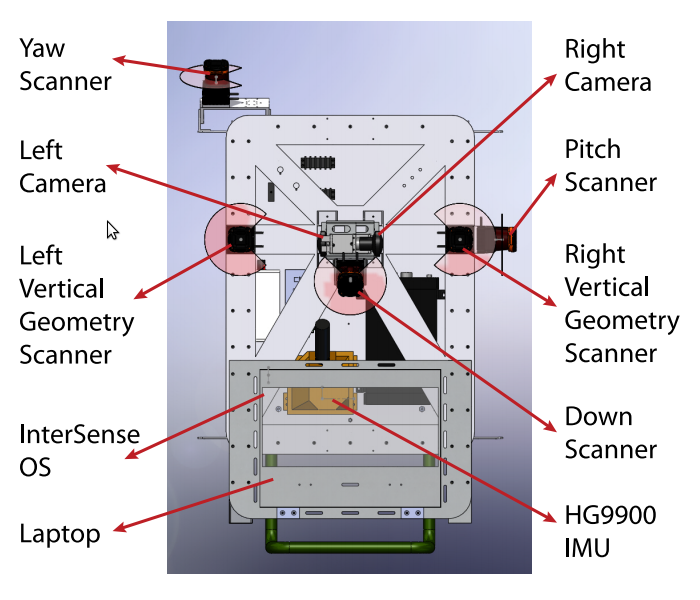
\includegraphics[width=3in]{backpackCAD.png}
  \caption{CAD model of the backpack system.}
  \label{fig:backpack}
\end{figure}

This section contains background information describing the
backpack-mounted system and its operation. The hardware and operation
of the backpack system, as well as the postprocessing of acquired
data, play an important role in motivating the approaches described in
this thesis. The following two sections will focus on image and raw
data acquisition, and a method of partitioning recovered environment
geometry, respectively.

\subsection{Acquisition Hardware}

A CAD model of the backpack-mounted system is shown in Figure
\ref{fig:backpack}. This backpack system has a number of laser range
scanners as well as 2 cameras facing left and right, each equipped
with fisheye lenses reaching an approximately 180$^{\circ}$ field of
view each and taking photos at a rate of 5 Hz \cite{liu2010indoor}. In
order to collect data, an operator wears the backpack system and
traverses the environment to be scanned, walking in straight lines at
a standard pace and making an effort to walk parallel to all walls in
the area. Multiple localization and loop-closure algorithms are then
applied to the raw data collected by the onboard sensors
\cite{chen2010indoor, kua2012loopclosure, liu2010indoor}, and the
backpack is localized\footnote{In this thesis, we use the terms
  localization and pose recovery interchangeably, in that they both
  refer to recovering position and orientation.}  over its data
collection period. This involves recovering the 6 degrees of freedom
for the backpack itself as well as the cameras rigidly mounted on it.
These results are noisy, which motivates the approaches in this
thesis. Once this is complete, the data from the laser range scanners
is used to generate a 3D point cloud of the surrounding
environment. This point cloud is used to construct either a
low-resolution planar model, such as for usage in basic navigation or
energy analysis \cite{sanchez2012point, turnerfloorplan}, or a
high-resolution, detailed mesh, for applications such as accurate
remodeling or virtual walkthroughs \cite{turnerwatertight}.
Regardless of resolution, size, or detail, the model, consisting of
geometric surfaces in 3D space, along with the set of images captured
by the backpack's cameras and their noisy 3D poses, are the input to
the texture mapping problem.

\subsection{Geometry Partitioning}
\label{sec:geometryPartitioning}

\begin{figure}
  \centering
  \subfloat[][]{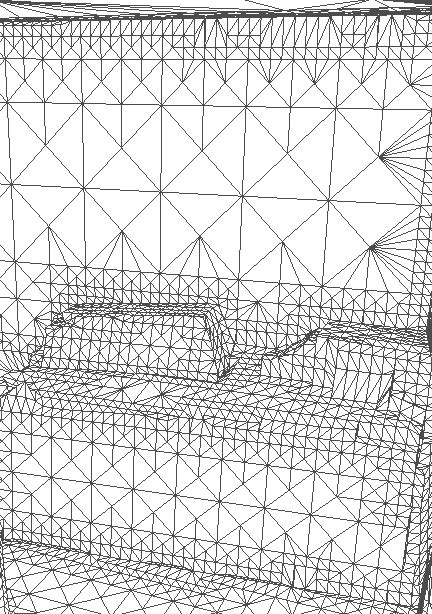
\includegraphics[width=2.2in]{geomdeskwire_crop.png}}
  \subfloat[][]{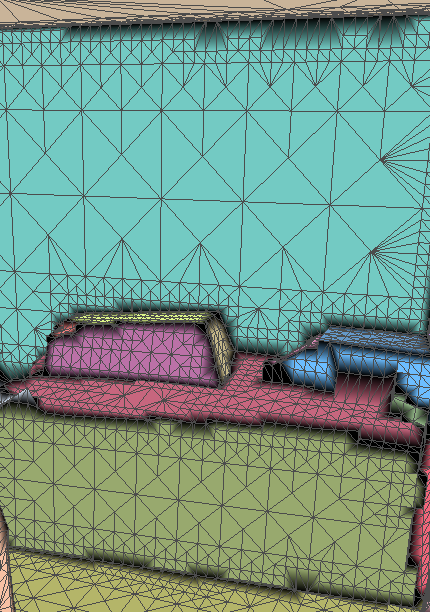
\includegraphics[width=2.2in]{geomdeskregions_crop.png}}
  \subfloat[][]{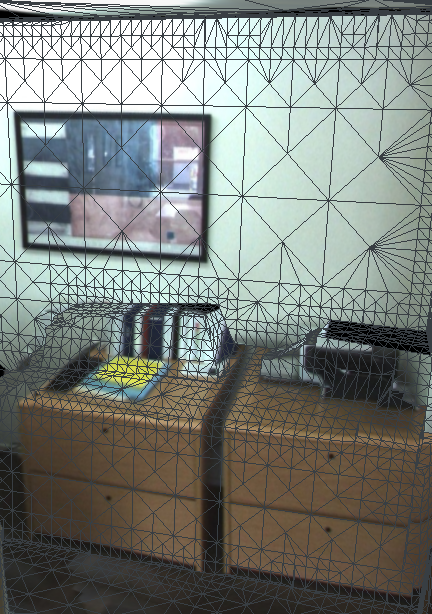
\includegraphics[width=2.2in]{geomdesktexturetris_crop.png}}
  \caption{(a) Part of a model representing a desk and miscellaneous
    objects on top of the desk. (b) Triangles grouped into regions for
    texturing. (c) Final textured output.}
  \label{fig:deskGeom}
\end{figure}


In order to effectively texture a 3D model, we first divide the model
into a set of regions, each to be textured independently. The purpose
of this is to ensure texture continuity along large uniform areas,
while allowing texture boundaries to fall along natural environmental
boundaries. Because textures may not match at such boundaries where
two regions meet, it is important to minimize the visibility of
boundaries. This is done by encouraging region boundaries to occur at
large sharp corners, where texture continuity is not important. When
working with lower-resolution models, where surfaces generally
correspond to large planar features such as walls, ceilings, or
floors, and often meet at right angles, each planar surface in the
model can simply be treated as a distinct region and textured
separately.

With high-resolution models however, geometry often represents large
features as well as small details found in furniture, plants, and
other miscellaneous objects. For instance, in Figure
\ref{fig:deskGeom}(a), the geometry modeling each side of a desk as
well as objects on top of it consists of many small triangles at
various orientations. It is important that triangles belonging to the
same object or surface are textured together, as texturing them
independently might lead to visible misalignment between the textures
of each triangle, resulting in poor visualizations. On the other hand,
triangles belonging to different objects, such as the wall vs. objects
on the desk need not be textured together, as texture alignment
between the two is not important in terms of overall visual quality of
the scene. Thus, in this example, the triangles comprising each side
of the desk, objects on top of the desk, and the wall behind, should
all be grouped into separate regions. This region grouping is done by
first designating all contiguous coplanar groups of triangles as
different regions. Any regions that are less than $1 m^2$ in size are
then joined to their largest neighboring regions, as long as the angle
between them is under $90^{\circ}$. An example of such a grouping is
shown in Figure \ref{fig:deskGeom}(b). The same area with textures
successfully applied to each region is shown in Figure
\ref{fig:deskGeom}(c).

Though some of these regions from high-resolution models are not
completely flat, a plane is fitted to each region for the purposes of
texturing. This plane corresponds to the largest contiguous section of
coplanar triangles, as most regions are characterized by small
outcroppings from a largely planar surface, such as objects on a table
or features protruding from a wall. The 3D surface composing a region
is then projected onto its calculated plane, and the resulting 2D
planar polygon is used as the texturing surface. This 2D planar
approximation provides a simple, yet approximately accurate surface
onto which images can be projected in order to generate
textures. However, 3D surfaces are still retained in order to achieve
more accurate results when performing occlusion checks during the
texturing process. To improve runtime during such occlusion checks,
the triangles within all 3D surfaces are also loaded into a k-d tree
for quick lookup. Thus, for high-resolution models, each region has
both 3D geometry stored in a k-d tree for occlusion purposes, and an
approximate 2D representation stored as the texturing surface.

At this point, we either have a series of planar regions from a low
resolution model, or a set of planar approximations for regions as
well as an associated k-d tree from a high resolution model. The task
now is to generate a texture for each region.

\section{Related Work}
\label{sec:relatedWork}
There are many existing approaches to stitching together multiple
images to produce a larger, seamless image \cite{szeliski2006image,
  agarwalapanoramas, wangmultipleviews, coorg1997matching,
  debevechybrid, bernardinimultiplescans}. Generally, parts of images
are matched to each other, either through direct comparisons at a
pixel level, or through feature detection and matching. Images are
then transformed to maximize matches, often by computing homographies
between pairs of images, or by iteratively adjusting camera poses in 1
to 6 degrees of freedom.

Feature matching has a number of advantages over direct matching that
make it more suitable for our often non-planar environments, and
rotational differences between camera poses
\cite{szeliski2006image}. Feature matching however, works best when
multiple unique visual references exist in the environment that can be
detected in multiple images. In contrast, indoor environments have a
high prevalence of bare surfaces, as well as repeating textures, such
as similar windows, doors, and wall-mounted decorations, that are
difficult to disambiguate. This lack of reliable reference points
often results in errors when matching images together.

Additionally, our datasets often contain long chains of images,
corresponding to long hallways and corridors as shown in Figure
\ref{fig:mosaic3D}, which leads to error accumulation when image
correspondences are not accurate. For example, when matching a long
chain of images through homography, a pixel in the $nth$ image must be
translated into the first image's coordinates by multiplying by the
$3\times3$ matrix $H_1 H_2 H_3 ... H_n$. Any error in one of these
homography matrices is propagated to all further images, resulting in
drift.

\begin{figure}
  \centering \subfloat[][]{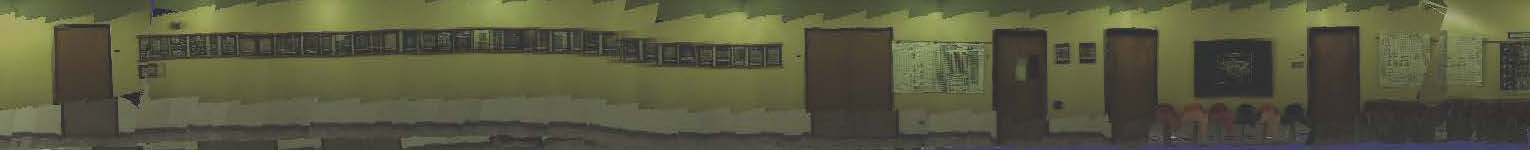
\includegraphics[trim=0cm 0cm 20cm 0cm,
    clip=true, width=6in, height=0.7in]{graphApproach.jpg}}

  \centering \subfloat[][]{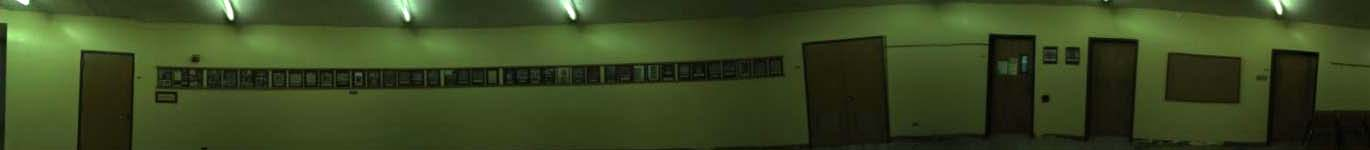
\includegraphics[trim=0cm 0cm 15cm 0cm,
    clip=true, width=6in, height=0.7in]{autostitchResult.jpg}}

  \centering \subfloat[][]{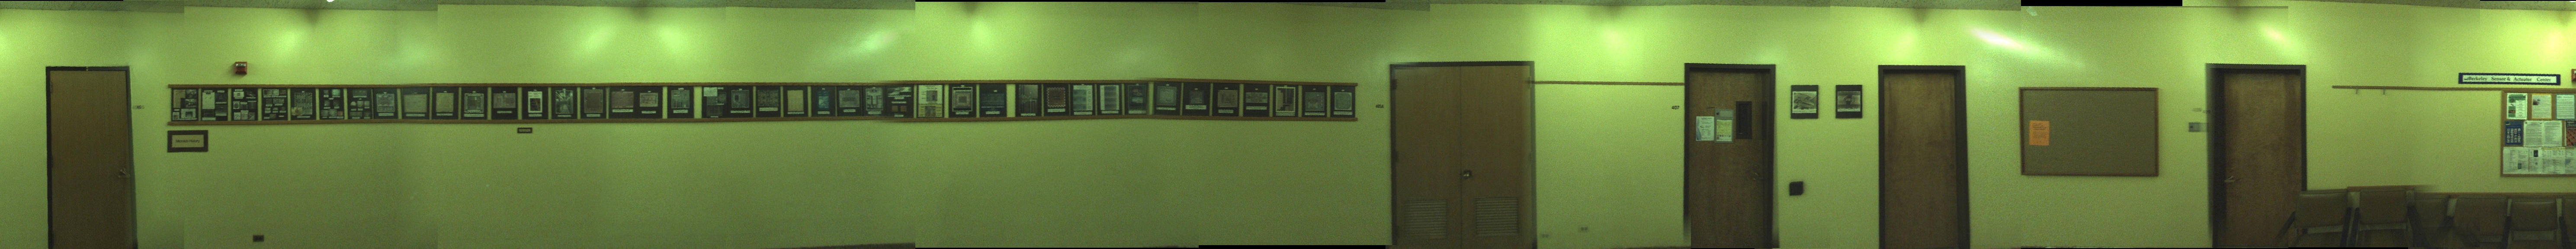
\includegraphics[trim=0cm 0cm 75cm 0cm,
    clip=true, width=6in, height=0.7in]{finalLong.jpg}}

  \caption{Texture alignment via (a) the graph-based localization
    refinement algorithm, (b) the AutoStitch software package, and (c)
    the proposed method.}
  \label{fig:mosaic3D}
\end{figure}


In prior work, we have experimented with integrating image stitching
with the iterative global localization algorithm used to recover the 6
degrees of freedom of the backpack acquisition system detailed in
Section \ref{sec:dataAcquisition} \cite{liu2010indoor}. When run on
long chains of images however, especially where features are sparse,
this approach produces distorted textures, as seen in Figure
\ref{fig:mosaic3D}(a). Furthermore, this approach is not closed-form,
and its iterative camera adjustment process over large datasets leads
to prohibitively long computation time.

The AutoStitch software package, based on research in the related area
of panorama genoration, also performs homography-based alignment, with
additional provisions that attempt to reduce drift and increase
overall efficiency \cite{panorama2d, autostitch}. Though AutoStitch
performs well in small areas, it often induces drift in images,
such that global alignment to the environment geometry is
lost. Furthermore, its performance relies on the presence of a dense
set of features, and it has trouble aligning wall sections with even
short segments of bare texture. The example in Figure
\ref{fig:mosaic3D}(b) was generated after many rounds of manual
tuning; we have empirically found that areas with fewer visual
features or repeating texture patterns simply failed outright with
AutoStitch.


\section{Image Selection}
\label{sec:imageSelection}

The geometry of the texture mapping process for a region, as described
in Section \ref{sec:geometryPartitioning}, is shown in Figure
\ref{fig:projection}. Given a set of images to texture a target
surface, camera matrix $P_i$ for the $i$th image transforms a 3D point
in the world coordinate system to a 2D point or pixel in image $i$'s
coordinates. A camera matrix $P_i$ is composed of the camera's
intrinsic parameters, containing focal length and image center, as
well as extrinsic parameters which specify the rotation and
translation of the camera's position in 3D world coordinates at the
time that image $i$ was taken. These extrinsic parameters are
determined by the backpack hardware and the corresponding localization
algorithms \cite{chen2010indoor, liu2010indoor, kua2012loopclosure}
and are noisy.

Since the backpack system takes pictures at a rate of 5 Hz, thousands
of images are available for texturing each surface in the 3D
model. Our objective in designing a texture mapping process is to
determine which of these images should be used, and where their
contents should map onto the final texture, in order to minimize any
visual discontinuities or seams that would suggest that the plane's
texture is not composed of a single continuous image. In the remainder
of this section, we propose an image subsampling procedure to obtain a
set of images for all further steps, and use it to derive a simple
tile-based texture mapping procedure.

\begin{figure}
  \begin{minipage}[b]{0.45\linewidth}
    \centering
    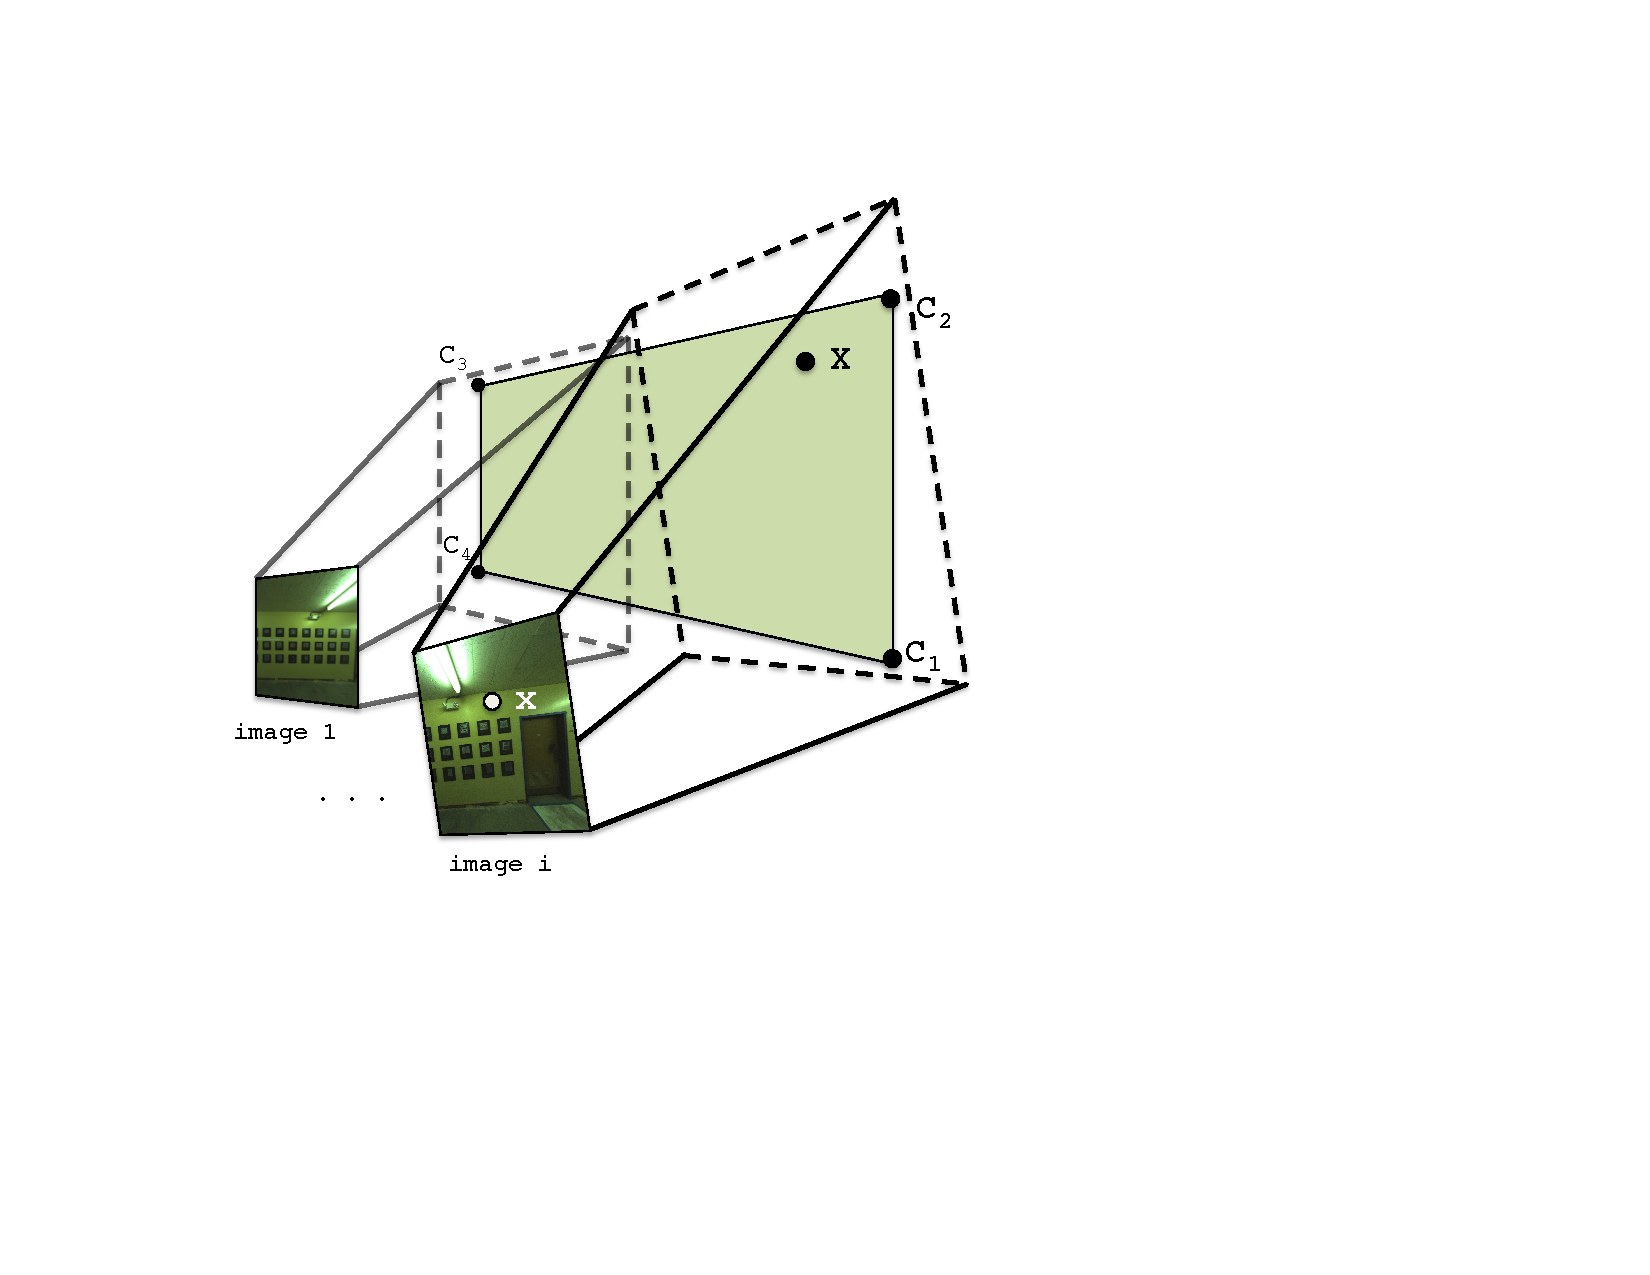
\includegraphics[height=1.8in]{Projection.pdf}
    \caption{Images are related to each surface through the camera
      matrices $P_{1..m}$. }
    \label{fig:projection}
  \end{minipage}
  \hspace{0.5cm}
  \begin{minipage}[b]{0.45\linewidth}
    \centering
    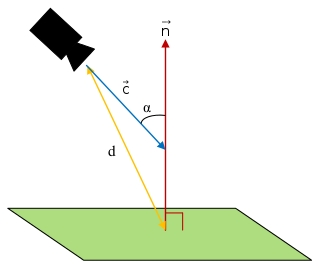
\includegraphics[height=1.8in]{scoringFunction.jpg}
    \caption{Camera angle $\alpha$ and distance $d$ are minimized by
      maximizing the scoring function $\frac{1}{d} (-1 \cdot \vec{c})
      \cdot \vec{n}$}
    \label{fig:scoringFunction}
  \end{minipage}
\end{figure}


Our criteria for image subsampling has the following
stipulations. First, we want a set of images such that their
projections together cover up the entirety of our target surface, so
as to avoid holes in the final texture. Second, we desire our final
texture to have high resolution throughout; thus every location on the
target surface should have at least one image that contains high
resolution imagery for it. A straightforward way to accomplish these
goals is to discretize the target surface into small square tiles, and
for each tile, select the image that has the best viewing angle and
resolution for texturing that tile. In order to select the image that
can best texture a tile $t$, we first gather a list of candidate
images that contain all four of its corners; we can rapidly check this
by projecting $t$ into each image using the $P_i$ camera
matrices. Furthermore, each candidate image must have been taken at a
time when its camera had a clear line-of-sight to $t$, which can be
determined using standard ray-polygon intersection tests between the
camera location, $t$, and every other surface, or via the k-d tree
from Section \ref{sec:geometryPartitioning} if present
\cite{rayintersection}.

Once we have a list of candidate images for $t$, we define a scoring
function in order to objectively select the best image for texturing
$t$. Since resolution decreases and camera pose errors become more
pronounced with distance, we wish to minimize the distance between
cameras and the surfaces they texture. Additionally, we desire images
that are projected perpendicularly, rather than obliquely, onto the
plane, maximizing the resolution and amount of useful texture
available in their projections, as well as minimizing any parallax
effects due to real-world geometry not accurately represented by the
digital 3D model. In other words, we wish to minimize the angle
between the tile's normal vector and the camera axis for images
selected for texturing that tile. These two criteria can be met by
maximizing the function $\frac{1}{d} (-1 \cdot \vec{c}) \cdot \vec{n}$
as shown in Figure \ref{fig:scoringFunction}, where $d$ is the
distance between the centers of a camera and a tile, and $\vec{n}$ and
$\vec{c}$ are the directions of the plane's normal and the camera axis
respectively.

When the images selected for each tile are used directly to texture
their respective tiles, image boundaries with abrupt discontinuities
between tiles are visible, as shown in Figure
\ref{fig:compareAll}(a). While it is clear that camera pose
inaccuracies are too severe for such a simple approach to work, the
selected images all appear to contain optimal camera angles with high
resolution, and much of their misalignment appears reconcilable using
2D transforms. This procedure generally selects around 10\% of the
possible images that could be used for texturing a surface, and not
only reduces the computational complexity of the remaining steps, but
also selects the most promising images for the remaining steps.



\begin{figure}
  \centering \subfloat[][]{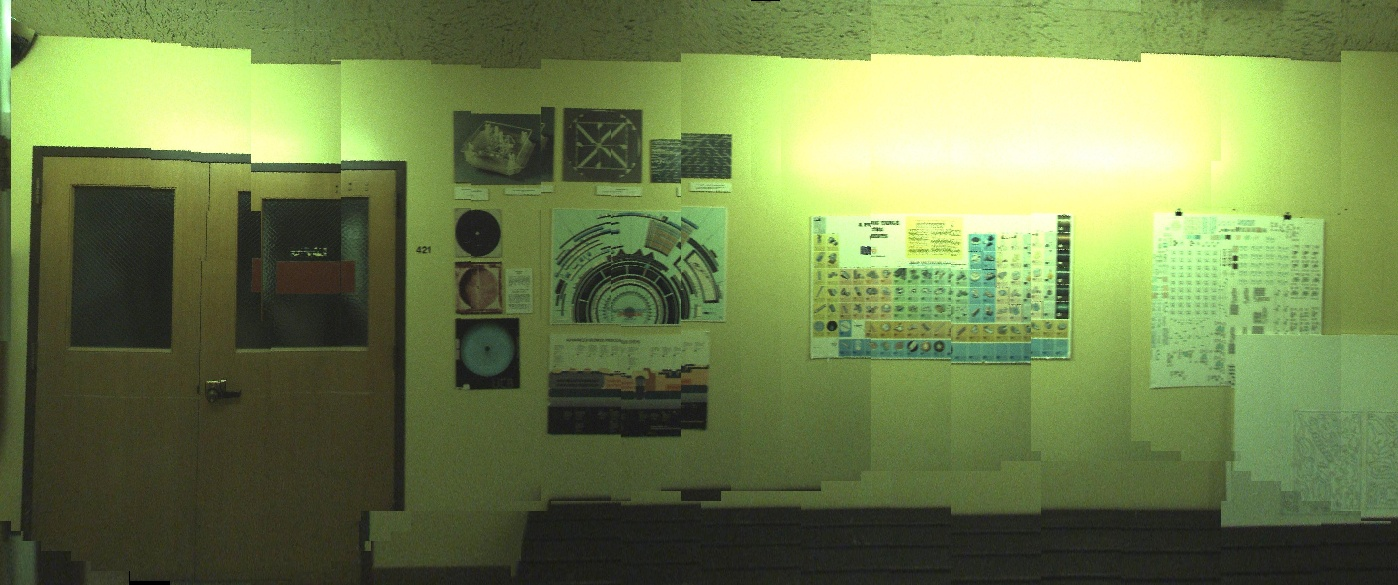
\includegraphics[width=3.4in,
    height=1.2in]{wall2_naive.jpg}}
  \subfloat[][]{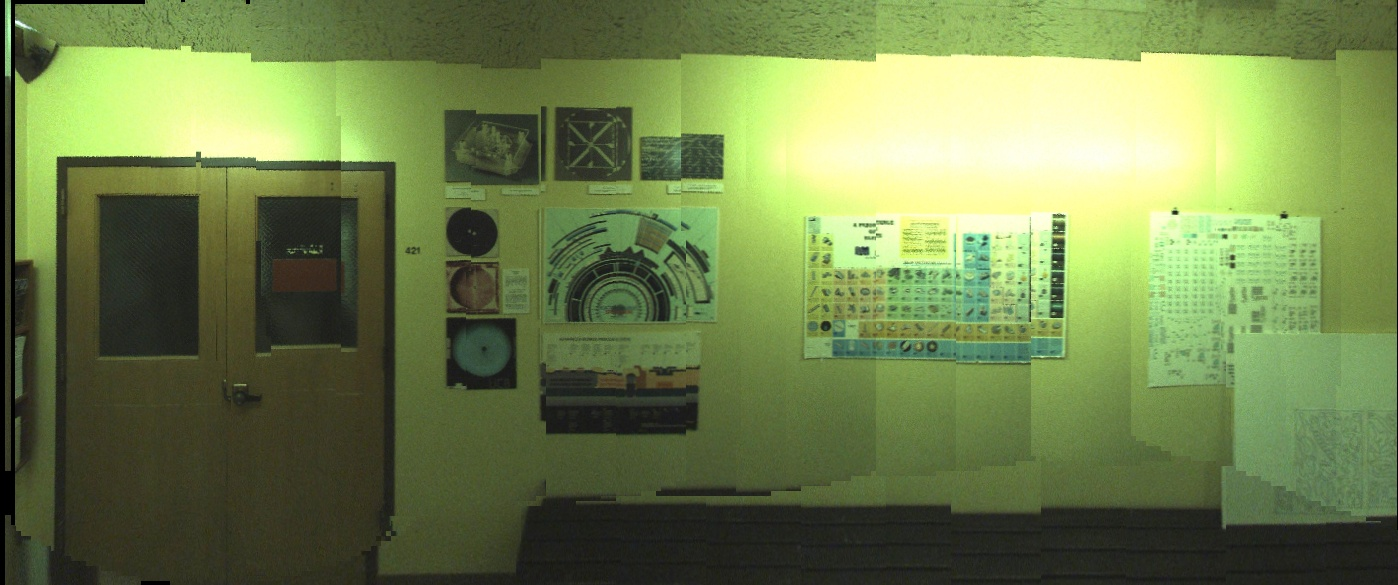
\includegraphics[width=3.4in,
    height=1.2in]{wall2_naive_shift.jpg}}

  \centering \subfloat[][]{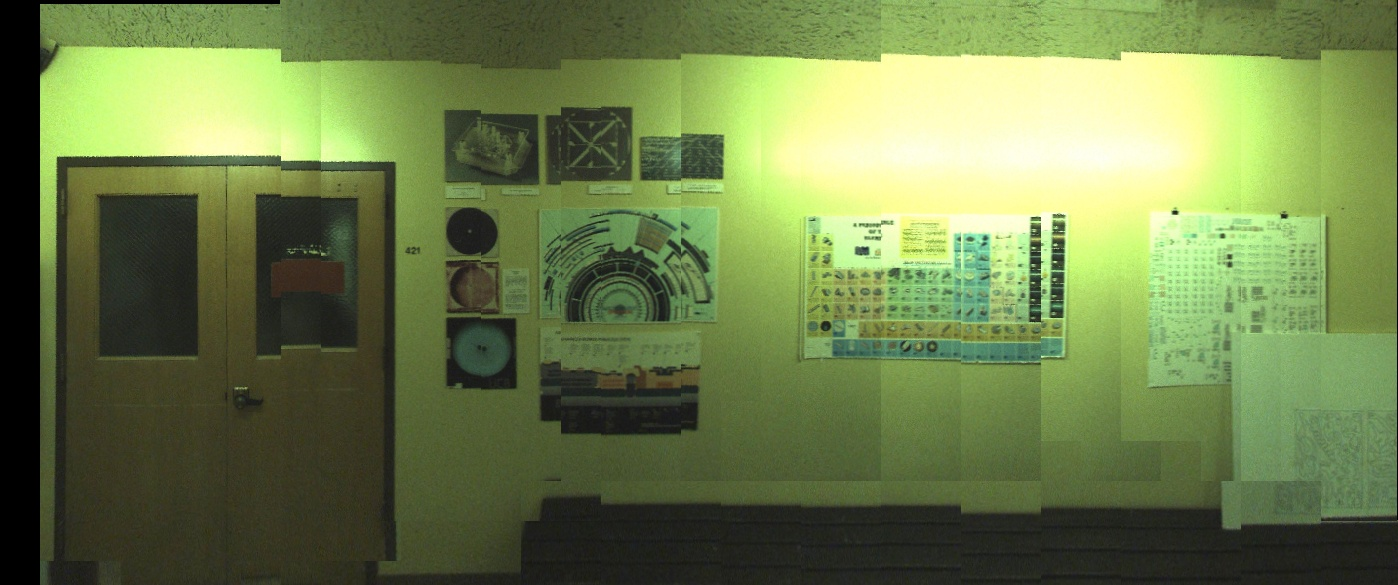
\includegraphics[width=3.4in,
    height=1.2in]{wall2_cache_shift.jpg}}
  \subfloat[][]{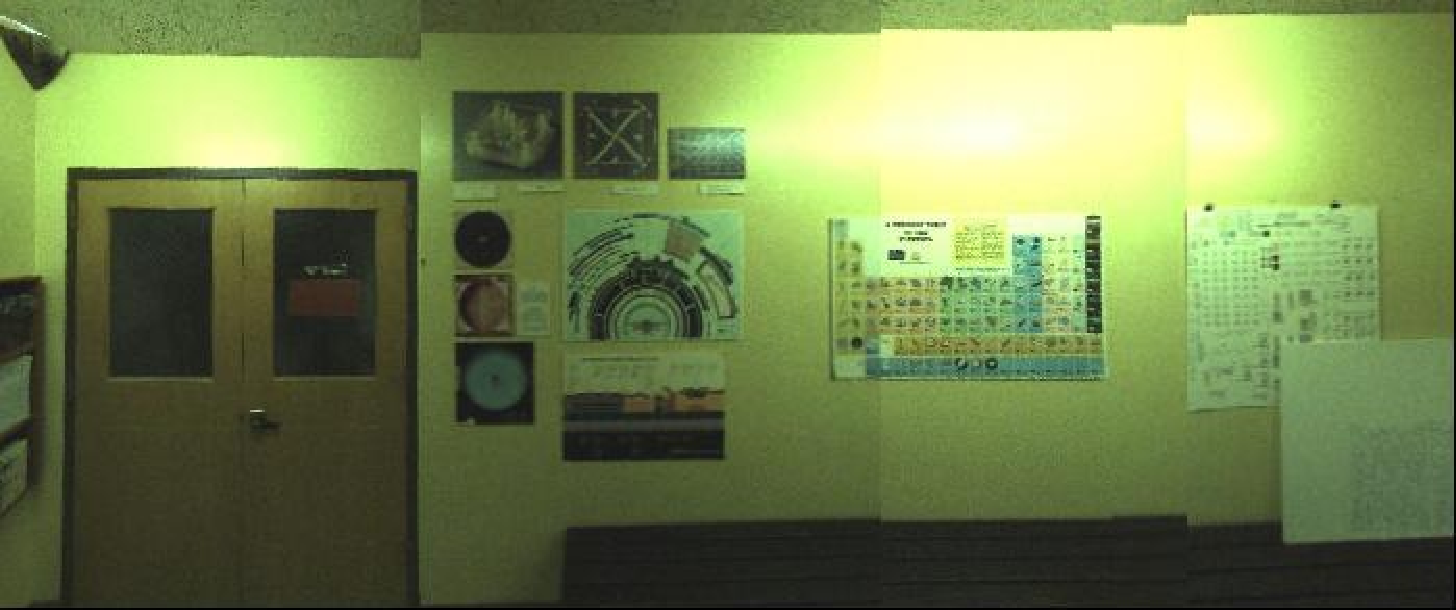
\includegraphics[width=3.4in,
    height=1.2in]{wall2_shortest_shift.pdf}}

  \centering \subfloat[][]{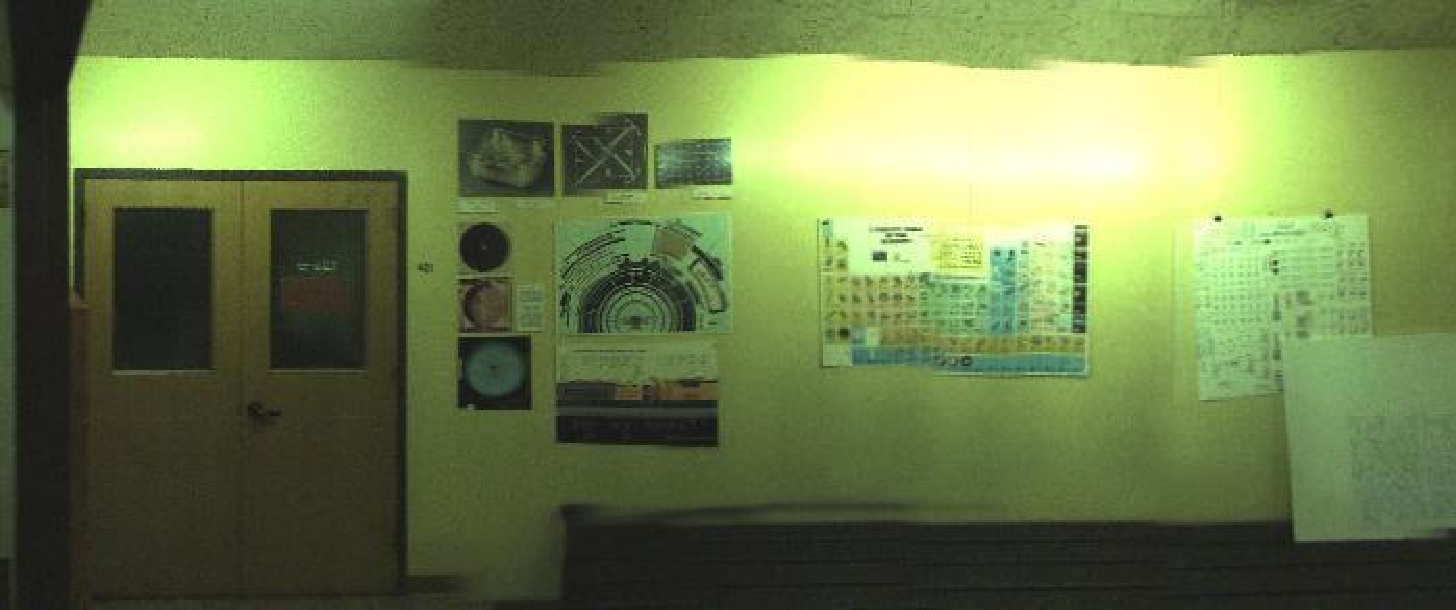
\includegraphics[width=3.4in,
    height=1.2in]{wall2_cache_shift_blend.pdf}}
  \subfloat[][]{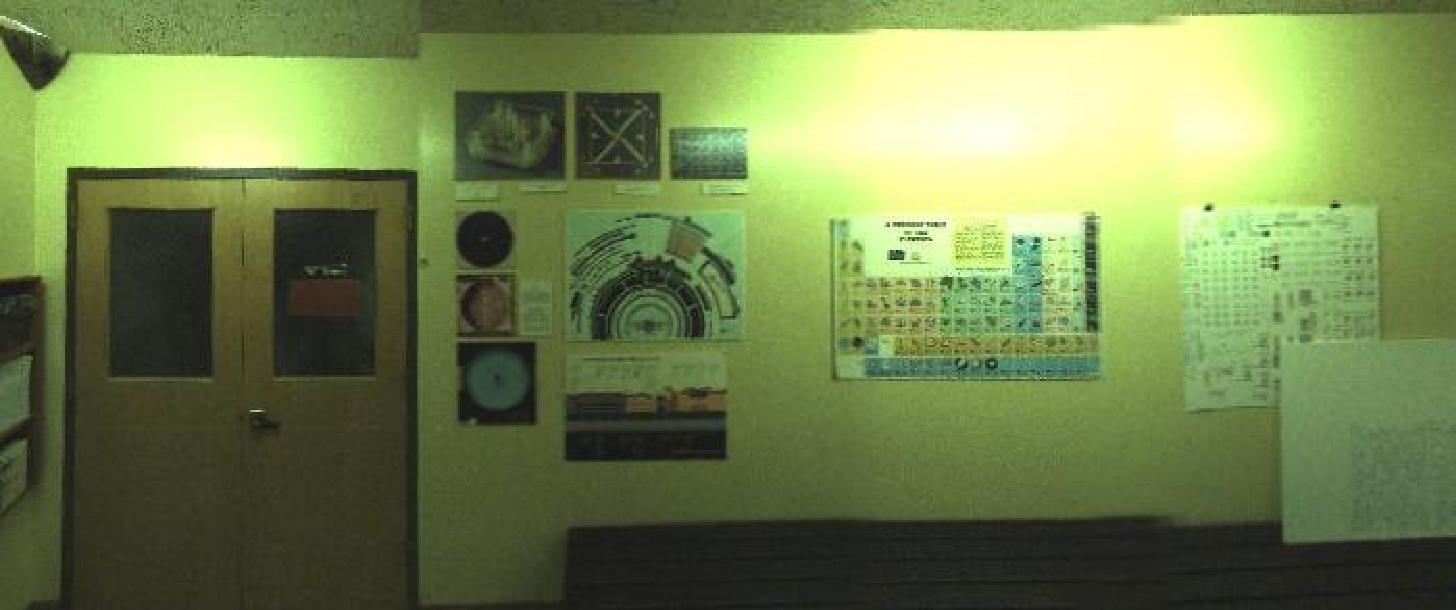
\includegraphics[width=3.4in,
    height=1.2in]{wall2_shortest_shift_blend.pdf}}

  \centering \subfloat[][]{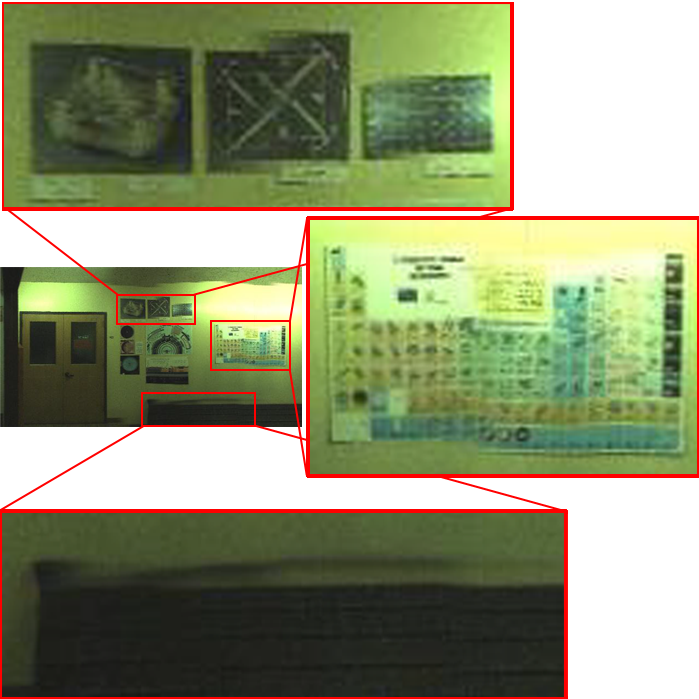
\includegraphics[width=3.4in,
    height=3.4in]{wall2_cache_comparison.png}}
  \subfloat[][]{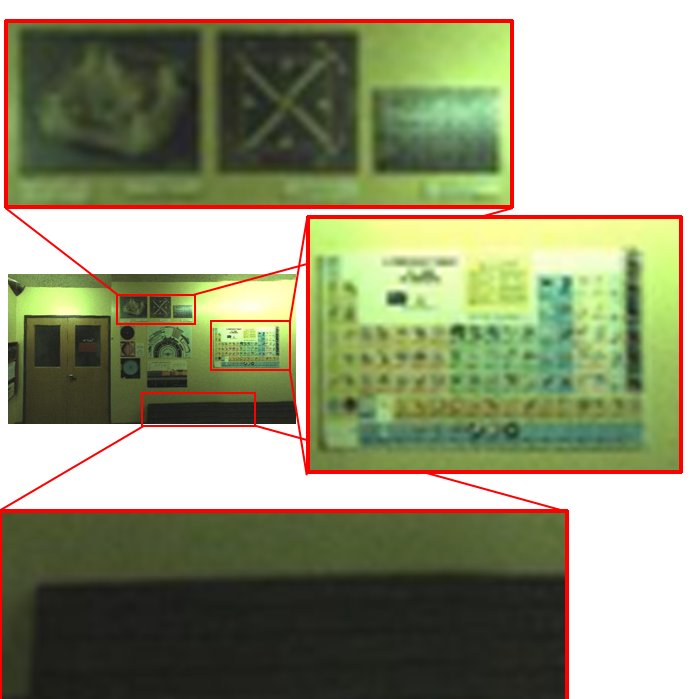
\includegraphics[width=3.4in,
    height=3.4in]{wall2_shortest_comparison.png}}

  \caption{(a) Tile-based texturing; (b) Tile-based texturing after
    image alignment; (c) Tile-based texturing after image alignment
    with caching; (d) Shortest path texturing after image alignment;
    (e,f) Blending applied to (c) and (d); (g,h) Zoomed in views of
    discontinuities in (e) vs. in (f).}
  \label{fig:compareAll}
\end{figure}


\section{2D Image Alignment}
\label{sec:2dAlignment}
In this section, we describe our method for efficient and robust image
alignment. Rather than register all of our images in 3D, as many
state-of-the-art techniques for image stitching do, we instead align a
subset of images in 2D; this subset corresponds to the images selected
by the image selection procedure described in Section
\ref{sec:imageSelection}.

Applying 2D alignments to this set of images works well for a number
of reasons. First, the nature of our input data and the selected
images is such that localization error chiefly occurs in two
dimensions, which correspond to the plane of most surfaces being
projected onto. This is because the backpack operator, during data
acquisition, makes efforts to walk within a few meters of, and
parallel to all walls being scanned. Furthermore, the backpack system
maintains a fairly consistent distance from floors and ceilings during
data collection. As a result, the translational error of camera poses
is quite minimal in dimensions perpendicular to most surfaces being
textured, corresponding to, or parallel to walls, ceilings and
floors. 

Our proposed 2D alignment procedure consists of three parts, as shown
in the diagram in Figure \ref{fig:flowchart}. First, images are
projected onto the surface and lines within these projected images are
detected. Images are then transformed such that these lines match
geometric lines composing the boundaries of the surface being
textured. Second, occlusion checks are performed to remove invalid
parts of each image for the target surface. Third, SIFT feature
matches are detected between pairs of images, and a weighted linear
least squares problem is solved in order to maximize all image and
geometry-based alignments. Each step will now be explained in detail.


\subsection{Geometry-based Alignment}
\label{sec:geometryAlignment}


\begin{figure}
  \centering
  \subfloat[][]{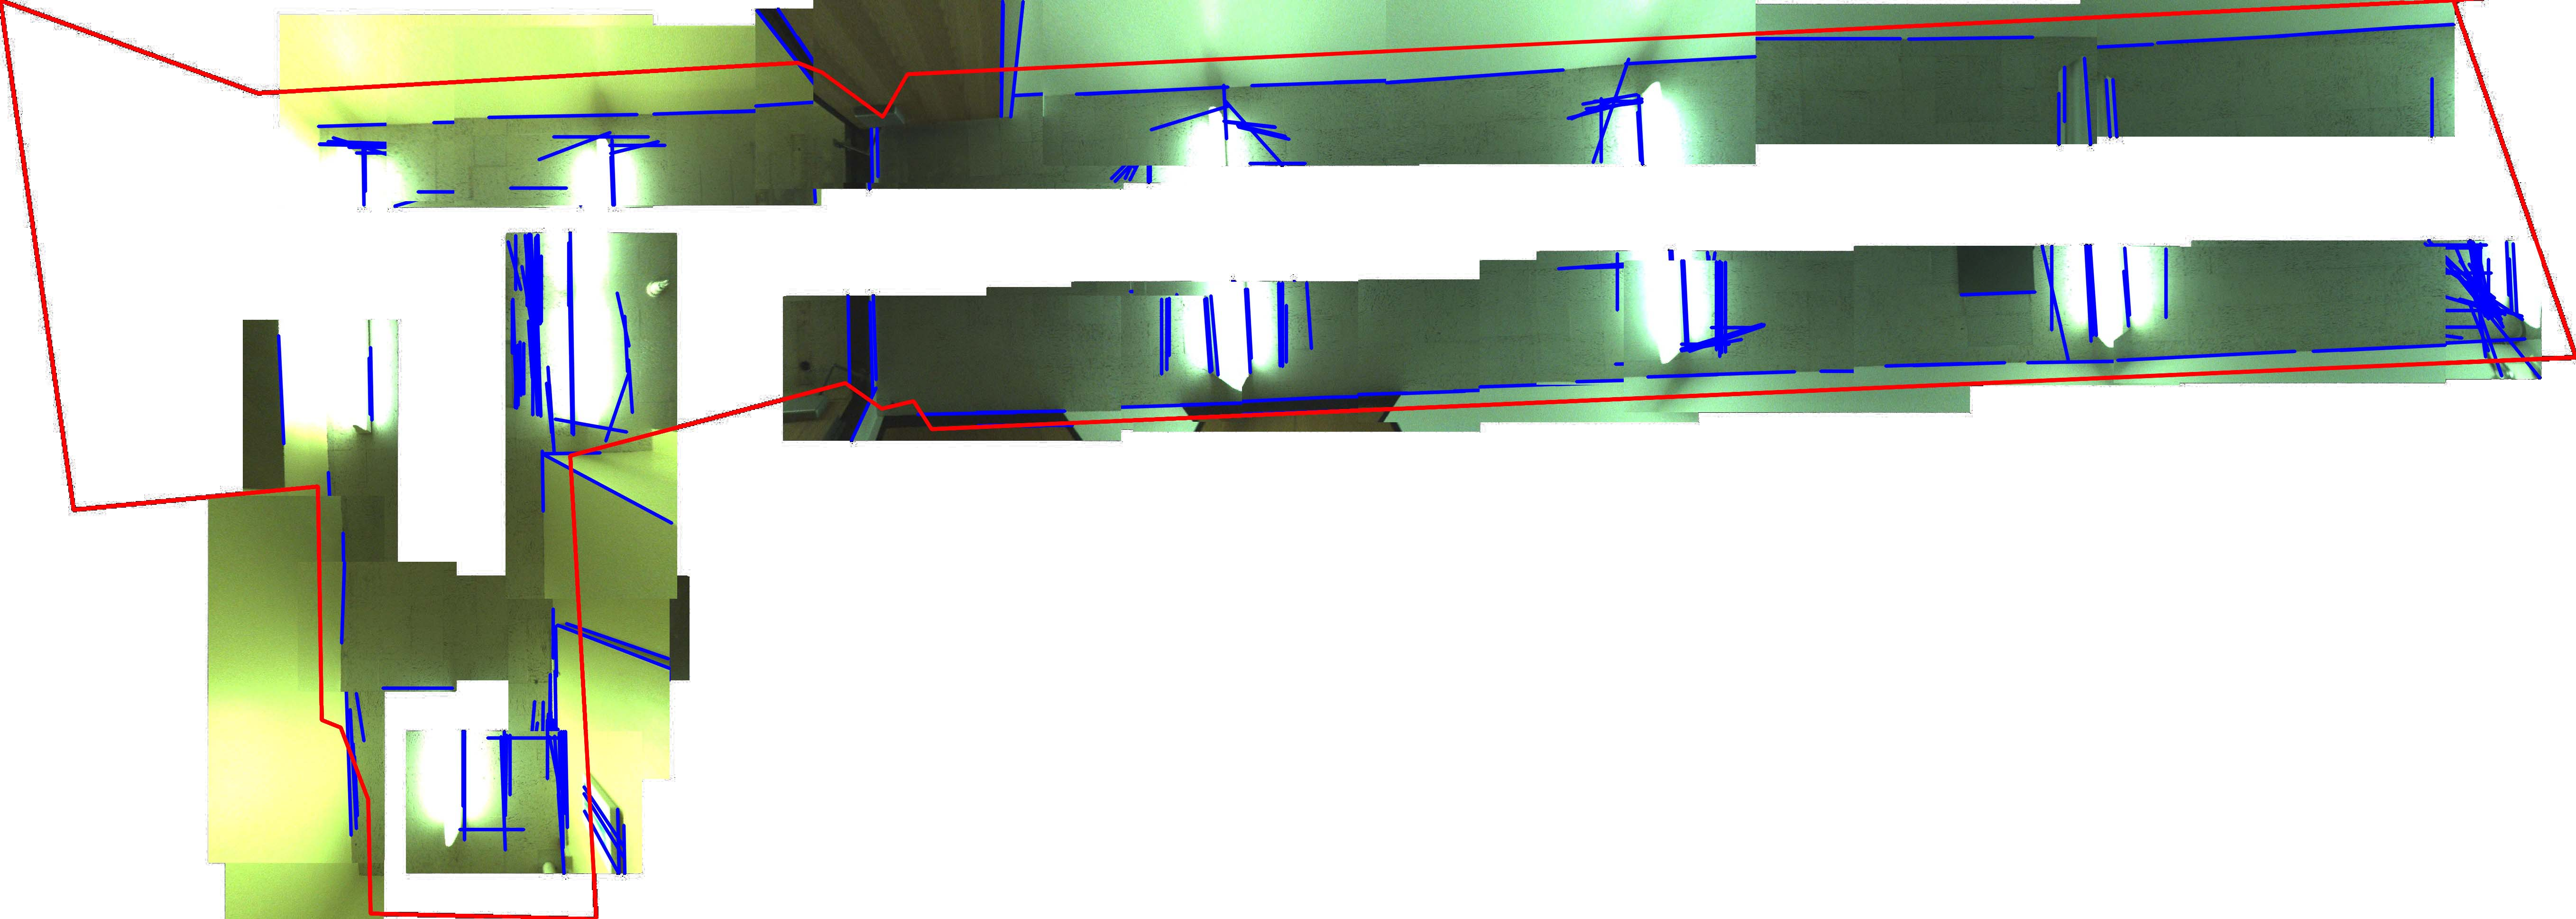
\includegraphics[width=6in]{allunshifted.jpg}}

  \centering
  \subfloat[][]{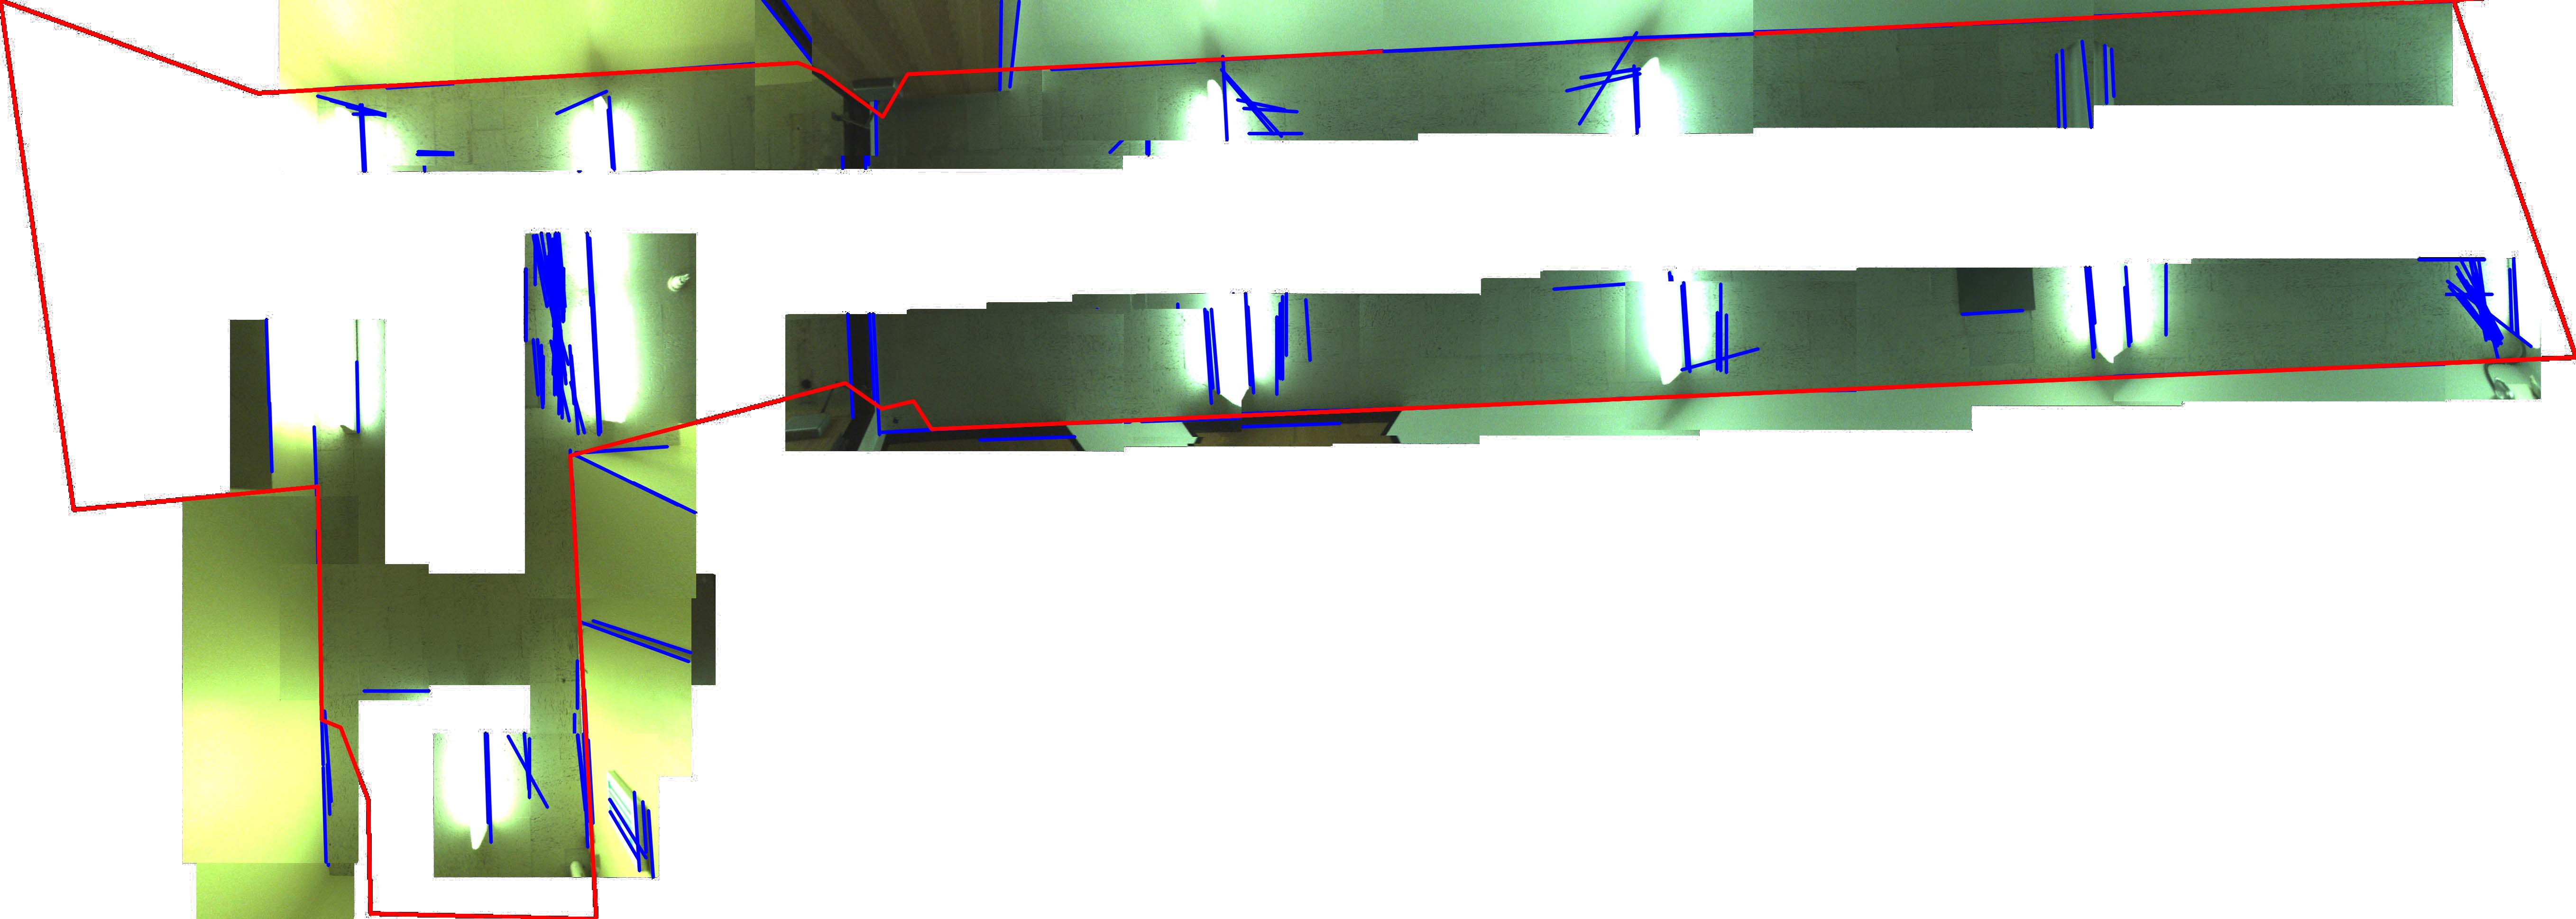
\includegraphics[width=6in]{allshifted.jpg}}

  \centering \subfloat[][]{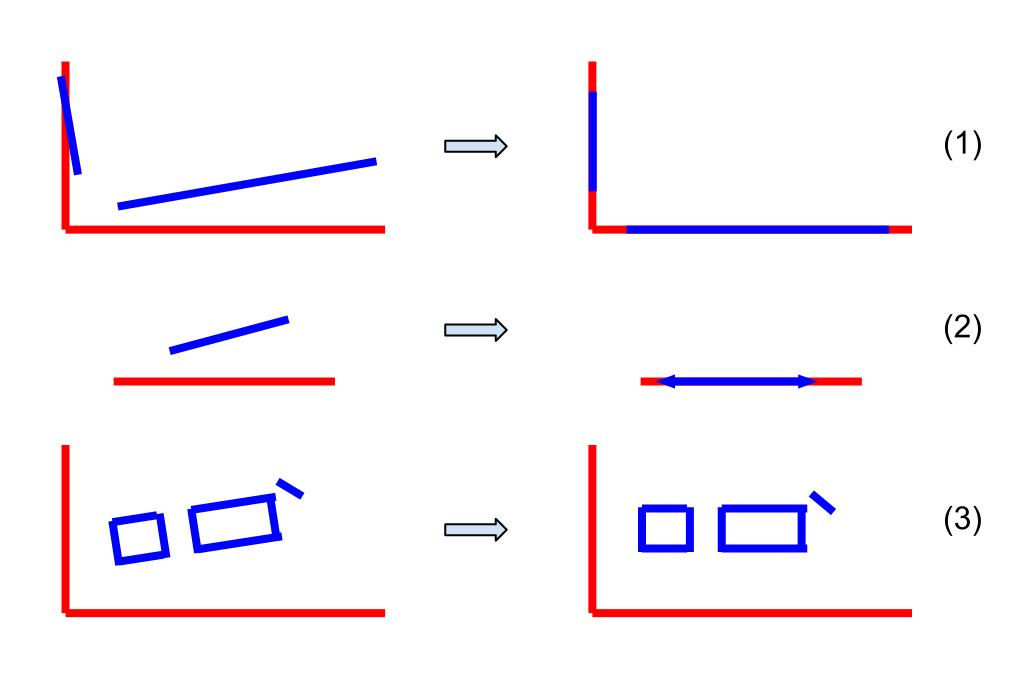
\includegraphics[trim=0cm 2cm 0cm 0cm,
    clip=true, width=5in]{matchLines.jpg}}

  \caption{Images projected onto a ceiling surface, where
    geometry-based lines corresponding to the ceiling's boundary are
    shown in red. Image-based lines detected by Hough transform in the
    image projections are shown in blue; (a) images projected with
    their original noisy camera poses; (b) after image alignment to
    maximize line matches between images and geometry; (c) examples of
    matching lines in cases with $\geq$ 2 line pairs, 1 line pair, and
    zero line pairs, from top to bottom.}
  \label{fig:geometryAlignment}
\end{figure}


After computing each image's projection onto the target surface, as
described in Section \ref{sec:imageSelection}, we can obtain a set of
image-based line segments by using Hough transforms to detect lines in
the image projections. These lines are detected in the image
projections rather than the original images, as the varying
orientation and distances of camera poses relative to surfaces results
in high variance of line lengths and strengths for real-world linear
features across the original images. We also gather a set of
geometry-based lines, which correspond to the lines comprising the
target surface's border, as well as lines formed where other surfaces
intersect the target surface. An example of these lines is shown in
red for a ceiling surface in Figure
\ref{fig:geometryAlignment}(a). Ideally, for perfect camera poses and
surface geometry, the lines in images corresponding to corners between
surfaces should match up exactly with corners in the 3D model. By
inducing such lines to match, we fit camera poses more accurately to
the surface, and to each other as well.

To align images to surface geometry, we collect pairs of image-based
and geometry-based line segments, which are within a distance and
angular difference threshold of each other. We have found a distance
threshold of 250 mm and an orientation difference threshold of
$10^\circ$ to work well for our datasets. For each pair of lines, we
compute the angular difference between the pair's image and geometry
lines. If there are 2 or more pairs with angular differences within
$1^\circ$, we select the two pairs with the longest noncollinear
image-based lines, and rotate the image such that the lines in the
pair with the longest image-based line become parallel. We then find a
translation such that the lines in that same pair overlap. This
translation has ambiguity in the dimension along the matched lines,
which is resolved by matching the midpoint of the image-based line in
the second pair to its corresponding geometry-based line. This is
shown in case (1) of Figure \ref{fig:geometryAlignment}(c). Thus, with
2 or more pairs, it is possible to obtain a fixed rotation and
translation for geometry alignment, which are saved for usage in
Section \ref{sec:robustSIFTFeatureMatching}.

If there are not 2 or more pairs with similar angular differences, we
select the pair with the longest image-based line, which corresponds
to a strong linear visual feature, and apply a rotation and the
minimal translation to match the pair's lines. This translation's
ambiguity however, can not be resolved, but is also saved to be used
in Section \ref{sec:robustSIFTFeatureMatching}. This is shown in case
(2) of Figure \ref{fig:geometryAlignment}(c). Finally, in the case
where there are no line pairs, we can still rotate images in order to
exploit patterns in indoor environments, as shown in case (3) of
Figure \ref{fig:geometryAlignment}(c). For instance, doors, windows,
furniture, etc. tend to have linear edges that are parallel to the
edges of the surfaces they are on. Similarly, lights, visible interior
walls, etc. which are visible in floor and ceiling images, tend to be
parallel to interior and exterior walls, corresponding to the
intersection lines and edges of ceiling and floor surfaces
respectively. Thus, we choose to minimize the angle between
image-based lines and geometry-based lines regardless of distance. We
use the RANSAC framework to compute a rotation angle that best
accomplishes this while ignoring outliers. \cite{fischler1981random}.

After these steps, image projections line up well with target
surfaces, as shown in Figure \ref{fig:geometryAlignment}(b), which is
considerably more aligned than Figure
\ref{fig:geometryAlignment}(a). This procedure reconciles both errors
in camera poses as well as in geometry, and results in sharp,
continuous borders across images, which is crucial when checking for
occlusion.


\subsection{Image Occlusion}
\label{sec:imageOcclusion}

\begin{figure}
  \centering
  \begin{tabular}{cc}
    \subfloat[][]{\raisebox{-1in}{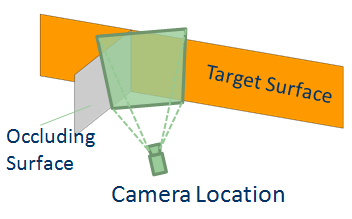
\includegraphics[width=3in]{occlusiondiagram.png}}} &
 
  \begin{tabular}{c}
    \subfloat[][]{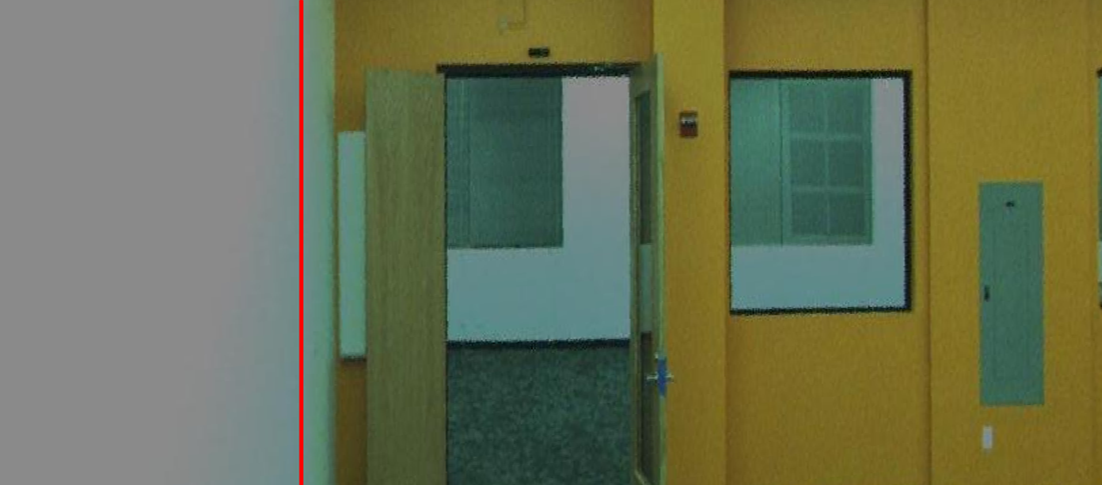
\includegraphics[trim=0cm 0cm 1.3cm 0cm,
      clip=true, width=3in,
      height=0.9in]{occlusionimagebad.png}} \\
    \subfloat[][]{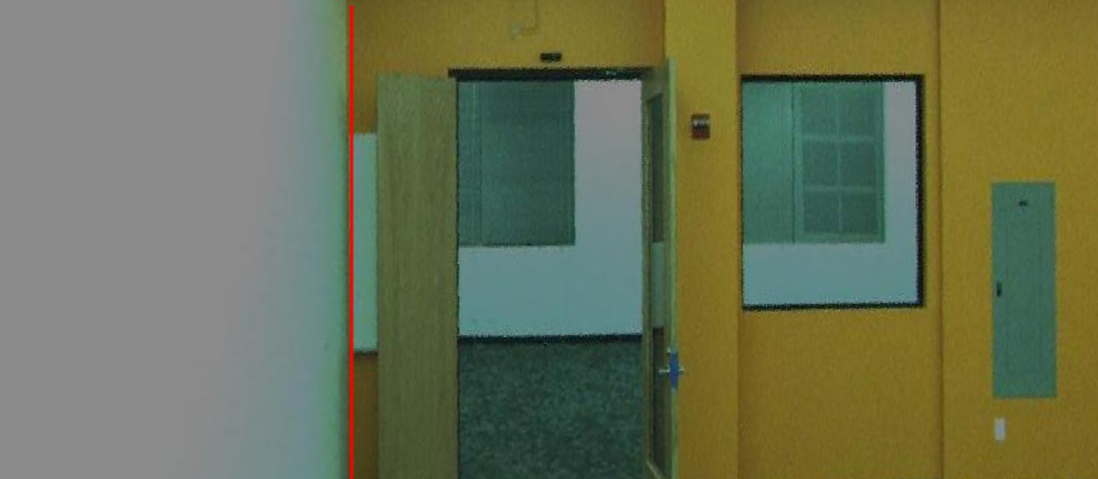
\includegraphics[trim=1.3cm 0cm 0cm 0cm,
      clip=true, width=3in,
      height=0.9in]{occlusionimagegood.png}}
  \end{tabular}
\end{tabular}
\caption{(a) The image from the camera in this diagram contains
  texture that belongs to the gray occluding surface, which should not
  be projected onto the orange target surface; (b) without geometry
  alignment, texture to the left of the red line would be removed,
  which would leave some erroneous texture projected onto our target
  surface; (c) after geometry alignment, the image is shifted,
  resulting in the correct amount of texture being removed.}
\label{fig:occlusion}
\end{figure}

In order to correctly texture surfaces, it is important to detect and
remove parts of image projections containing texture for occluding
surfaces. For instance, in Figure \ref{fig:occlusion}(a), an image
used to texture the orange target surface also contains part of a gray
occluding surface. We remove this incorrect texture by recursively
performing ray-polygon intersection tests between the camera location
and every surface in our model except the target surface
\cite{rayintersection}. If using planar approximations for regions, as
explained in Section \ref{sec:geometryPartitioning}, the k-d tree is
used instead. These intersection tests are performed at the corners of
a grid overlaid upon the target surface. Where all four corners of a
grid section are occluded, texture is removed. Where one or more
corners are occluded, the grid is subdivided into four, and the
process repeats. Occlusion checking works entirely with geometry, so
by ensuring that images match geometry using
\ref{sec:geometryAlignment}'s alignment procedure, texture belonging
to other surfaces is accurately removed, as seen in Figure
\ref{fig:occlusion}(b) vs. \ref{fig:occlusion}(c).

\subsection{2D Feature Alignment}
\label{sec:robustSIFTFeatureMatching}
The next step is to align the selected images from Section
\ref{sec:imageSelection} for each surface to each other by searching
for corresponding feature points between all pairs of overlapping
images. We use feature alignment rather than pixel or intensity-based
alignment due to the differences in lighting as well as possible
occlusion among images, both of which feature alignment is less
sensitive to \cite{lowe1999object, mikolajczyk2005performance,
  szeliski2006image}. We use SiftGPU \cite{siftgpu} for its high
performance on both feature detection as well as pairwise
matching. These matches determine $dx$ and $dy$ distances between each
pair of features for two image projections, though these distances may
not always be the same for different features. Since indoor
environments often contain repetitive features such as floor tiles or
doors, we need to ensure that SIFT-based distances are
reliable. First, we only align parts of images that overlap given the
original noisy poses. Second, we discard feature matches that
correspond to an image distance greater than 200 mm from what the
noisy poses estimate. In order to utilize the remaining feature
matches robustly, RANSAC \cite{fischler1981random} is again used to
estimate the optimal $dx_{i,j}$ and $dy_{i,j}$ distances between two
images $i$ and $j$. We use a 5 mm threshold for RANSAC, so that SIFT
matches are labeled as outliers if their distance is not within 5 mm
of the sampled average distance.

We now use the feature-based distances between each pair of images as
well as geometry alignment results from Section
\ref{sec:geometryAlignment} to refine all image positions using a
weighted linear least squares approach. An example setup for a
weighted linear least squares problem $\textrm{min}_{\vec{\beta}}
||W^\frac{1}{2}(A \vec{\beta} - \vec{\gamma})||_2^2 $ with 3 images is
as follows.

\[
A =
\begin{pmatrix}
  -1 & 1 & 0 & 0 & 0 & 0\\
  0 & 0 & 0 & -1 & 1 & 0\\
  0 & -1 & 1 & 0 & 0 & 0\\
  0 & 0 & 0 & 0 & -1 & 1\\
  0 & -m_2 & 0 & 0 & 1 & 0\\
  1 & 0 & 0 & 0 & 0 & 0\\
  0 & 0 & 0 & 1 & 0 & 0\\
  1 & 0 & 0 & 0 & 0 & 0\\
  0 & 0 & 0 & 1 & 0 & 0\\
  0 & 1 & 0 & 0 & 0 & 0\\
  0 & 0 & 0 & 0 & 1 & 0\\
  0 & 0 & 1 & 0 & 0 & 0\\
  0 & 0 & 0 & 0 & 0 & 1\\


\end{pmatrix}\quad
\vec{\beta} =
\begin{pmatrix}
  x_1, \\ x_2, \\ x_3, \\ y_1, \\ y_2, \\ y_3
\end{pmatrix}
\vec{\gamma} =
\begin{pmatrix}
  dx_{1,2}, \\ dy_{1,2}, \\ dx_{2,3}, \\ dy_{2,3}, \\ -m_2gx_2 + gy_2,
  \\ gx_1, \\ gy_1, \\ tx_1, \\ ty_1, \\ tx_2, \\ ty_2, \\ tx_3, \\
  ty_3
  
\end{pmatrix}
\vec{W} =
\begin{pmatrix}
  1, \\ 1, \\ 1, \\ 1, \\ 1, \\ 1, \\ 1, \\ 0.01, \\ 0.01, \\ 0.01, \\
  0.01, \\ 0.01, \\ 0.01
\end{pmatrix}
\]


The variables we wish to solve for are the $x_i$ and $y_i$ positions
of images, while equations are the feature-based distances between
pairs of images, images fixed to geometry with 0 or 1 degrees of
freedom, and the original noisy camera poses. In this scenario, a
feature-based distance of $dx_{1,2}$, $dy_{1,2}$ was calculated
between images 1 and 2. This corresponds to the first and second row
of $A$, while the third and fourth row of $A$ represent the same for
images 2 and 3. Rows 5 through 7 correspond to results of the geometry
alignment procedure in Section
\ref{sec:geometryAlignment}. Specifically, row 5 corresponds to a
geometry-based constraint of image 2's location to a line of slope
$m_2$, passing through point $gx_2$, $gy_2$, while rows 6 and 7
correspond to a fixed location for image 1 without any degrees of
freedom. Rows 8 through 13 correspond to the original camera locations
for each image ($tx_i,ty_i$).

The original camera poses are needed due to lack of feature matches in
all images, or lack of enough geometry alignment results to generate a
single solution. Since it is desirable to minimally use the original
noisy poses, we assign to them a weighting factor of $0.01$, while all
other equations are weighted at $1$.

Since this problem is linear, it can be solved efficiently; after
applying the resulting shifts, images overlap and match each other
with far greater accuracy. Using the simple tile-based texturing
scheme from Section \ref{sec:imageSelection} on these adjusted images
results in Figure \ref{fig:compareAll}(b), which has far fewer
discontinuities than in \ref{fig:compareAll}(a), though some 3D error
as well as lighting differences and parallax effects are still
visible.

\section{Image Compositing}
\label{sec:imageCompositing}
In Section \ref{sec:imageSelection} we described an image selection
method that reduces the list of candidate images for texturing by a
factor of 10. In this section we go one step further to choose a
subset of the above candidates in order to further reduce visual
artifacts and discontinuities across textured surfaces. Specifically,
in Section \ref{sec:mappingWithCaching}, we refine the tile-based
texturing approach from Section \ref{sec:imageSelection}, with an
added caching mechanism to reduce image boundaries. This method is
general and works well given arbitrary camera poses and surfaces,
whether large planar surfaces or small geometric interior
features. For special cases where images have consistently
perpendicular viewing angles to the surfaces under consideration, such
as walls, it is possible to develop an alternative method in Section
\ref{sec:shortestPath} to further reduce visual artifacts. Both of
these approaches are followed by a blending step in order to produce
final textures for each surface, as shown in Figure
\ref{fig:flowchart}.

\subsection{Tile-Mapping with Caching}
\label{sec:mappingWithCaching}
For the simple texture mapping method described in Section
\ref{sec:imageSelection}, discontinuities occur where adjacent tiles
are textured by different images. Though Section
\ref{sec:2dAlignment}'s image alignment removes many such
discontinuities, there are still cases where seams are visible due to
imprecise matching or other factors such as model-based errors as
shown in Figure \ref{fig:compareAll}(b). To reduce this, it is
desirable to develop a spatiotemporal caching mechanism to take into
account image selections made by neighboring tiles while texture
mapping a given tile. By using the same image across tile boundaries,
it is possible to eliminate a discontinuity altogether. If a tile is
not visible in images used by neighboring tiles, using similar images
across tile boundaries also leads to less noticeable discontinuities.

The best image for a tile $t$ is selected by searching through two
subsets of images for a viable candidate, before searching through the
entire set of valid images obtained in Section
\ref{sec:imageSelection}. The first subset of images is those selected
by adjacent tiles that have already been textured. We must first check
which of these images contain texture for $t$, and then of those, we
make a choice according to the scoring function in Figure
\ref{fig:scoringFunction}. Before reusing this image, we check the
criteria $\alpha < 45^\circ$, in order to ensure a high resolution
projection, with $\alpha$ as the camera angle as shown in Figure
\ref{fig:scoringFunction}.

If no satisfactory image is found in the first subset, we check a
second subset of images, consisting of those taken near the ones in
the first subset, both spatially and temporally. We use the noisy
camera poses to determine spatial proximity. These images are not the
same as the ones used for neighboring tiles, but are taken at a
similar location and time, suggesting that their localization and
projection are quite similar, and thus likely match more
seamlessly. If no viable image is found according to the $\alpha <
45^\circ$ criteria, we search the entire set of candidate images from
Section \ref{sec:imageSelection}, selecting based on the same scoring
function from Figure \ref{fig:scoringFunction}.

The result of applying this caching approach to the images for the
surface in Figure \ref{fig:compareAll}(a) is shown in Figure
\ref{fig:compareAll}(c), where seams are considerably reduced as
compared to Figure \ref{fig:compareAll}(b). However, some
discontinuities are still present, as visible in the posters on the
wall with breaks in their borders.

\begin{figure}
  \centering
  \subfloat[][]{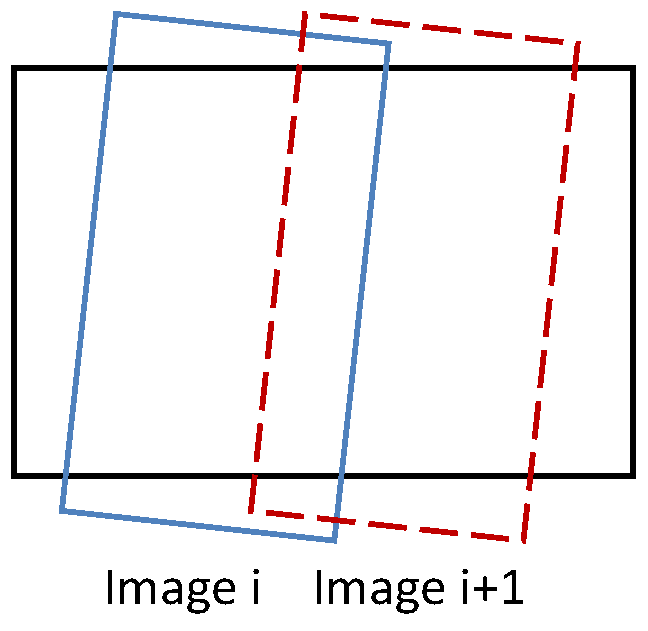
\includegraphics[width=1.5in]{projectionWall.pdf}}
  \hspace{0.51in} \centering
  \subfloat[][]{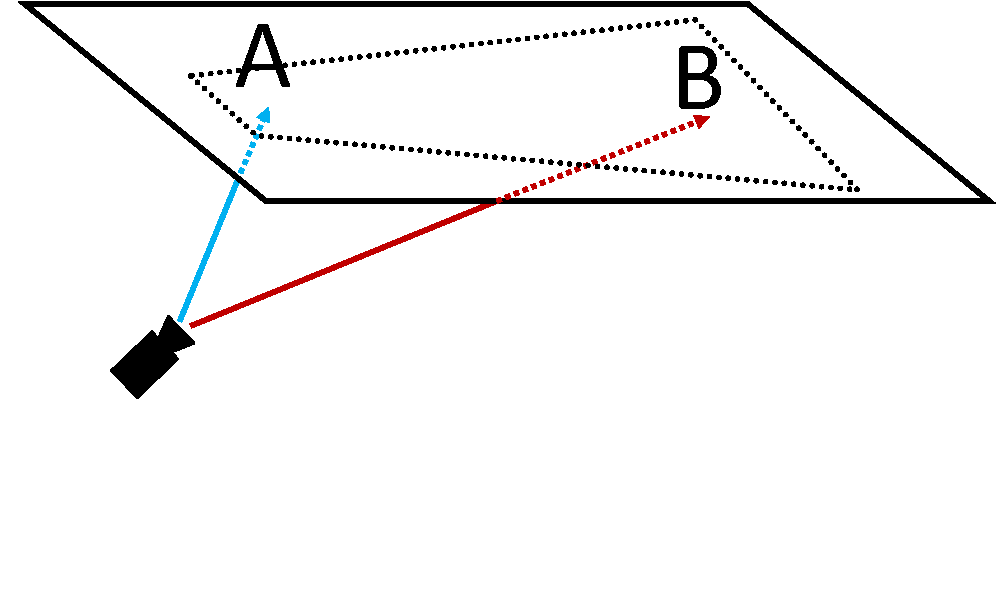
\includegraphics[width=1.5in]{projectionCeiling.pdf}}
  \centering \hspace{0.5in}
  \subfloat[][]{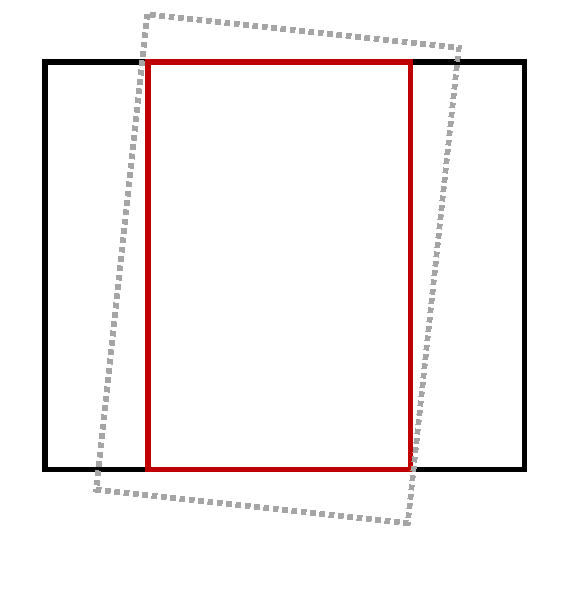
\includegraphics[width=1.5in]{projectionWallCrop.pdf}}
  \caption{(a) Images for vertical planes are tilted, but their camera
    axes are more or less normal to their respective planes. (b)
    Camera axes for ceiling images are at large angles with respect to
    plane normals. (c) Wall images are cropped to be rectangular.}
  \label{fig:projectionAngles}
\end{figure}

\subsection{Shortest Path Texturing}
\label{sec:shortestPath}

As mentioned earlier, our data comes from a mobile backpack system
carried by am ambulatory human operator, typically bent forwards at 15
to 20 degrees with respect to the vertical direction. As a result,
cameras facing sideways are head on with respect to vertical surfaces,
as shown in Figure \ref{fig:projectionAngles}(a), while cameras
oriented towards the top or bottom of the backpack are at an angle
with respect to floors, ceilings and other horizontal surfaces, as
shown in Figure \ref{fig:projectionAngles}(b). These oblique camera
angles for horizontal surfaces translate into textures that span large
areas once projected, as shown in Figure
\ref{fig:projectionAngles}(b). Using the tile-based texture mapping
criteria from Figure \ref{fig:scoringFunction}, such projections have
highly varying scores depending on the location of a tile on the
plane. Thus, the tiling approach in Section
\ref{sec:mappingWithCaching} is an appropriate choice for texturing
horizontal surfaces, as it uses the parts of image projections that
maximize resolution for their respective plane locations, e.g. areas
near point A and not near point B, in Figure
\ref{fig:projectionAngles}(b).

For vertical surfaces however, which make up a large portion of most
models, images are usually taken from close distances and head-on
angles, resulting in high resolution fronto-parallel projections. As a
result, for each tile on a wall plane, the scoring function of Figure
\ref{fig:scoringFunction} is relatively flat with respect to candidate
images, as they are all more or less head on. Since the scoring
function is less discriminative for walls, it is conceivable to devise
a different texturing strategy to directly minimize visible seams when
texturing them. This is done by choosing the smallest possible subset
of images from the set selected in Section \ref{sec:imageSelection}
and aligned in Section \ref{sec:2dAlignment} such that it (a) covers
the entire plane and (b) minimizes the visibility of borders between
the images. A straightforward cost function that accomplishes the
latter is the sum of squared differences (SSD) of pixels in
overlapping regions between all pairs of images. Minimizing this cost
function encourages image boundaries to occur either in featureless
areas, such as bare walls, or in areas where images match extremely
well.

In its most general form, our problem can be defined as minimally
covering a polygon i.e. the planar surface, using other polygons of
arbitrary geometry i.e. image projections, with the added constraint
of minimizing the cost function between chosen images. Given that
wall-texture candidate images are taken from more or less head-on
angles, and knowing that only minor rotations are made in Section
\ref{sec:2dAlignment}, we can crop our image projections to be
rectangular with minimal texture loss as shown in Figure
\ref{fig:projectionAngles}(c). Furthermore, because the fisheye camera
lenses have full floor-to-ceiling coverage of nearly all walls, and
the backpack operator logically only moves horizontally, we only need
to ensure lateral coverage of our wall planes. We can thus construct a
Directed Acyclic Graph (DAG) from the images, with edge costs defined
by the SSD cost function, and solve a simple shortest path problem to
find an optimal subset of images with regard to the SSD cost function
\cite{dijkstra}.

\begin{figure}
  \centering
  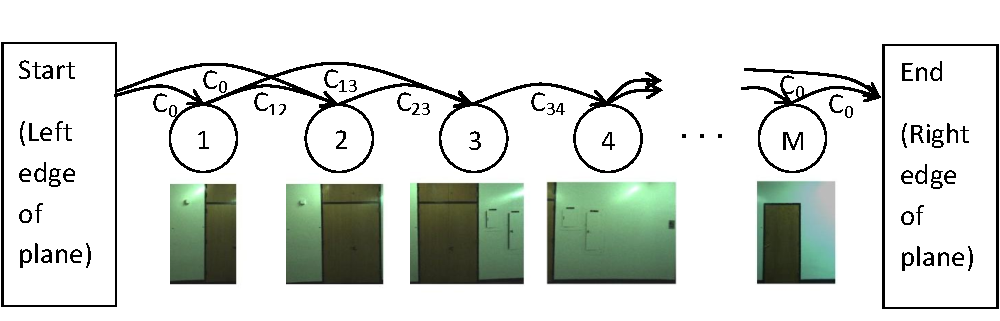
\includegraphics[width=4in]{dagCreation.pdf}
  \caption{DAG construction for the image selection process. \\}
  \label{fig:dagCreation}
\end{figure}

Figure \ref{fig:dagCreation} demonstrates the construction of a DAG
from overlapping images of a hallway wall. Images are sorted by
horizontal location left to right, and become nodes in a
graph. Directed edges are placed in the graph from left to right
between overlapping images. The weights of these edges are determined
by the SSD cost function. Next, we add two artificial nodes, one start
node representing the left border of the plane, and one end node
representing the right border of the plane. The left(right) artificial
node has directed edges with equal and arbitrary cost $C_0$ to(from)
all images that meet the left(right) border of the plane. We now solve
the shortest path problem from the start node to the end node. This
results in a set of images completely covering the plane horizontally,
while minimizing the cost of seams between images.

We have now (a) mapped every location on the plane to at least one
image, (b) decreased the number of texturing images, generally
retaining around 20\% of the image subset obtained in Section
\ref{sec:imageSelection}, and (c) decreased the discontinuities at
each image border. As seen in Figure \ref{fig:compareAll}(d), this
shortest path method has fewer visible discontinuities than Figure
\ref{fig:compareAll}(c) corresponding to the tile caching
approach\footnote{In Figure \ref{fig:compareAll}(d), we arbitrarily
  chose one image for texturing where images overlap, as blending will
  be discussed in section \ref{sec:blending}.}. This is especially
evident when comparing the posters in the images. This shortest path
approach approach directly reduces the cost of each image boundary,
while the tile caching method uses a scoring function that only
approximates this effect. Furthermore, this approach guarantees the
best selection of images to minimize seams, while the sequential tile
caching method may select images early on that turn out to be poor
choices once subsequent tiles have been processed. This shortest path
approach is also far less intensive in terms of memory usage and
runtime, both during texture generation and rendering, as it does not
require discretizing planes or images.

When texturing a model, we apply the shortest path method on vertical
surfaces, due to its superior results when provided with head-on
images. Floors, ceilings, and smaller complex objects such as
furniture, given their many images taken at oblique angles, are
textured using the tile caching method of Section
\ref{sec:mappingWithCaching}.

\subsection{Exposure Compensation}
\label{sec:exposureCompensation}

\begin{figure}
  \centering
  \subfloat[][]{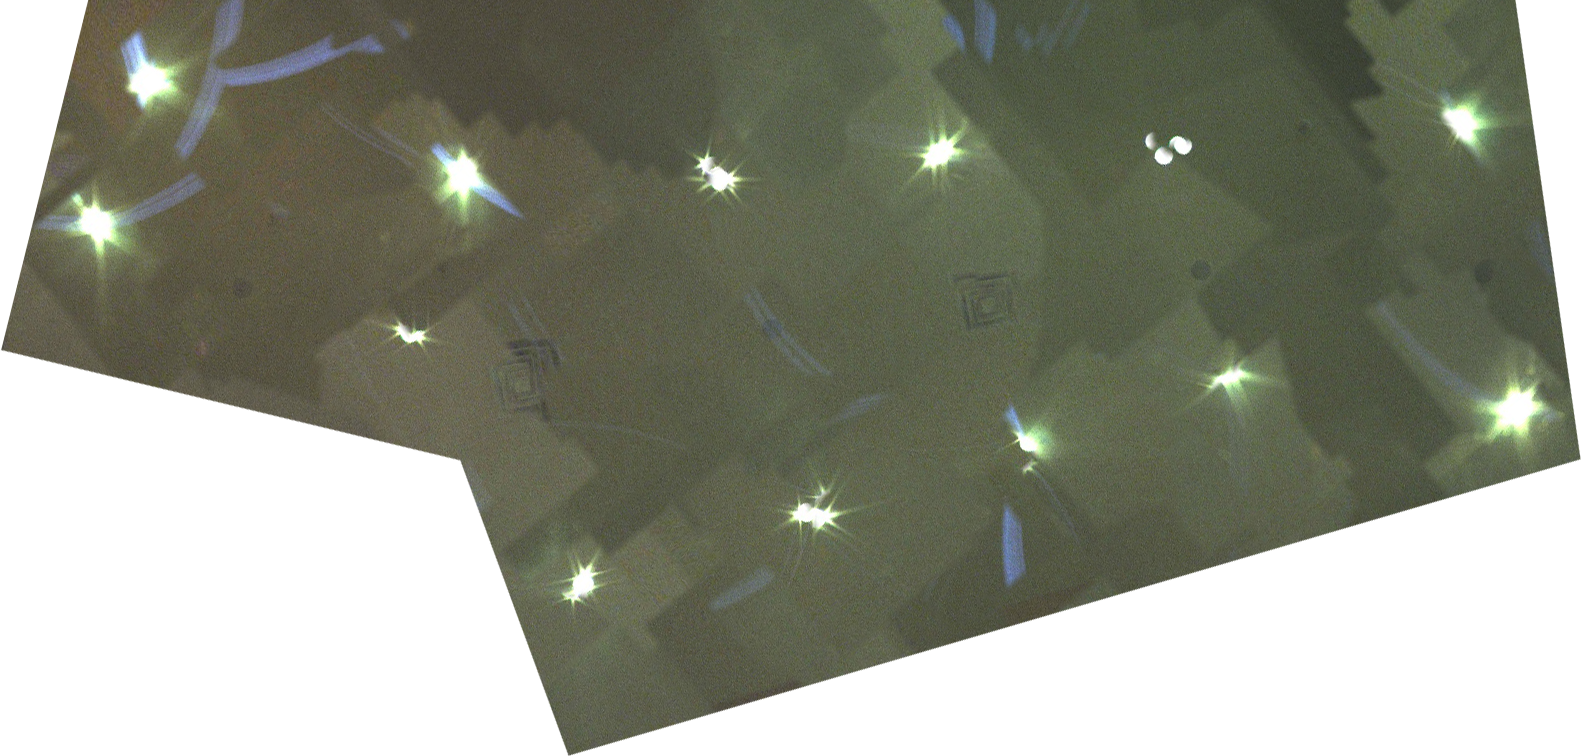
\includegraphics[width=3.3in]{exposureDiff1.png}}
  \subfloat[][]{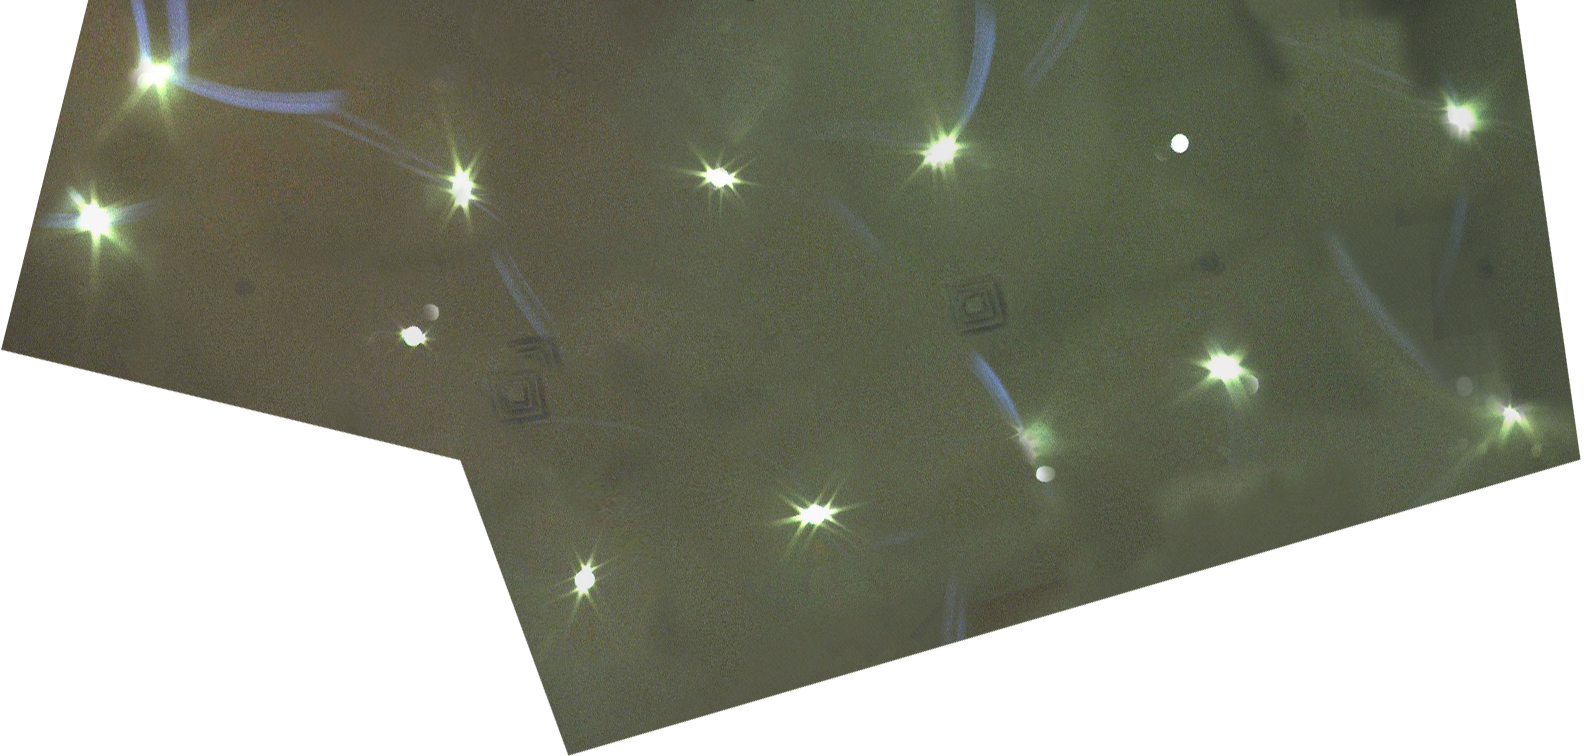
\includegraphics[width=3.3in]{exposureDiff2.png}}
  \caption{(a) A ceiling texture composed of images taken with varying
    exposures, with significant brightness differences. (b) Exposure
    compensation applied to the same set of images from (a) by
    applying computed gains to each image}
  \label{fig:exposureDiff}
\end{figure}


Before blending images together, exposure compensation is applied to
equalize brightness among neighboring images. For the images in this
report, cameras are set to have automatic exposure, which means that
images of the same object may have different brightness levels. While
successful image alignment and blending can reduce sharp seams between
adjacent images, there may still be noticeable brightness gradients
between images, particularly in areas near light sources. This can be
seen in Figure \ref{fig:exposureDiff}(a), where the ceiling texture
has patches of clearly differing brightness. To diminish this effect,
a gain can be computed and applied to each image, with the effect of
linearly scaling the brightness of each image. The goal is to compute
a gain for each image, such that the brightness of an area is
consistent across image boundaries.

Similar to the image position refinement procedure in Section
\ref{sec:robustSIFTFeatureMatching}, exposure compensation is
performed simulatenously across all images present in a single
region. As before, this is solved as a least-squares optimization
problem with pair-wise observations. In this case, observations do not
need to be weighted, and so the formulation is
$\textrm{min}_{\vec{\beta}} ||(A \vec{\beta} - \vec{\gamma})||_2^2
$. An example setup for 3 images, each with 2 overlapping pixels, is
shown below.
\[
A =
\begin{pmatrix}
  P_{11} & -P_{12} & 0\\
  P_{21} & -P_{12} & 0\\
  0 & P_{32} & -P_{33}\\
  0 & P_{42} & -P_{43}\\
  1 & 1 & 1\\

\end{pmatrix}\quad
\vec{\beta} =
\begin{pmatrix}
  G_1, \\ G_2, \\ G_3
\end{pmatrix}
\vec{\gamma} =
\begin{pmatrix}
  0, \\ 0, \\ 0, \\ 0, \\ 3
\end{pmatrix}
\]

In this problem, $\beta$ is the vector of gains $G_i$ to be solved
for.  The observations, represented by $A$ and $\gamma$, correspond to
equalizing the brightness for each pixel present in two images. For
instance, for pixel $P_x$ which is present in two overlapping images
$I_i$ and $I_j$, the goal is to find gains $G_i$ and $G_j$ such that
$G_iP_{xi} - G_jP_{xj} = 0$, where $P_{xy}$ is the value of pixel
$P_x$ in image $I_y$. Thus, $\gamma$ contains all zeros, while each
row of $A$ contains a $P_{xi}$ value in the $ith$ column and a
$-P_{xj}$ value in the $jth$ column, and zeros elsewhere. This problem
is not constrained, as it allows all computed gains to be scaled by
any amount. To keep gains at reasonable values, a final observation is
added: $\Sigma G_i = N$, where $N$ is the number of images. This has
the effect of setting the average of all gains to 1, and is
represented by adding a row of ones to $A$, and a corresponding $N$
value to $\gamma$.

The result of computing and applying gains for each image can be seen
for the same ceiling location in Figure \ref{fig:exposureDiff}(b). As
compared to Figure \ref{fig:exposureDiff}(a), the effect is clear, as
dark/bright patches are no longer present, and the overall brightness
of the image has not changed significantly.

\subsection{Blending}
\label{sec:blending}
We now apply a blending procedure to the texturing methods in Sections
\ref{sec:mappingWithCaching} and \ref{sec:shortestPath}. Although the
image alignment and selection steps in both methods attempt to
minimize all mismatches between images, and exposure compensation
minimizes brightness differences, there are occasional unavoidable
discontinuities in the final texture due to parallax effects or
inaccuracies in model geometry. These can however be treated and
smoothed over by applying alpha blending over image seams.  Whether
the units to be blended are rectangularly-cropped images or
rectangular tiles, we can apply the same blending procedure, as long
as there is a guaranteed overlap between units to blend over.

For the tile caching method of Section \ref{sec:mappingWithCaching},
we can ensure overlap by texturing a larger tile than needed for
display. For example, for a rendered tile of size $l_1 \times l_1$, we
can associate it with a texture $(l_1 + l_2) \times (l_1 + l_2)$ in
size.  We have found $l_2 = \frac{l_1}{2}$ to provide a good balance
between blending and keeping features unblurred at image
boundaries. For the shortest path method, we already have ensured
overlap between images. To enforce consistent blending however, we add
a minimum required overlap of images of 200 mm while solving the
shortest path problem in Section \ref{sec:shortestPath}. Additionally,
if images overlap in a region greater than the overlap distance, we
only apply blending over an area equal to the overlap distance.

After linear alpha blending across overlapping regions, the texture
mapping process is complete. Figures \ref{fig:compareAll}(e) and
\ref{fig:compareAll}(f) show the blended versions of Figures
\ref{fig:compareAll}(c) and \ref{fig:compareAll}(d) respectively. The
remaining images in Figure \ref{fig:compareAll} highlight differences
between the two methods, showing that Figure \ref{fig:compareAll}(f)
has the best visual quality and the best texturing approach among the
textures in Figure \ref{fig:compareAll}.



\section{Results}
\label{sec:results}
This section contains results of the proposed texture mapping process
on a number of different environments, with geometry generated using
three different methods. Further images of individual textured
surfaces and entire textured models, as well as videos and interactive
walkthroughs can also be found at
\footnote{\url{http://www-video.eecs.berkeley.edu/research/indoor/}}.

\subsection{Examples}
\label{sec:examples}
As mentioned in Section \ref{sec:dataAcquisition}, the texture mapping
procedure in this thesis can be applied both to low-resolution and
high-resolution models. Low resolution models have an advantage in
their simplicity, and in that only important environmental features
are represented. As a result, images are generated for large sections
of buildings, and texture continuity is maintained over large
areas. High resolution models have an obvious advantage in terms of
the amount of detail that can be reconstructed, but with poor region
partitioning, as described in Section \ref{sec:geometryPartitioning},
or with high camera pose or geometry reconstruction error, 3D elements
in the environment geometry may not match up well with their imaged
counterparts.

\begin{figure}
  \centering
  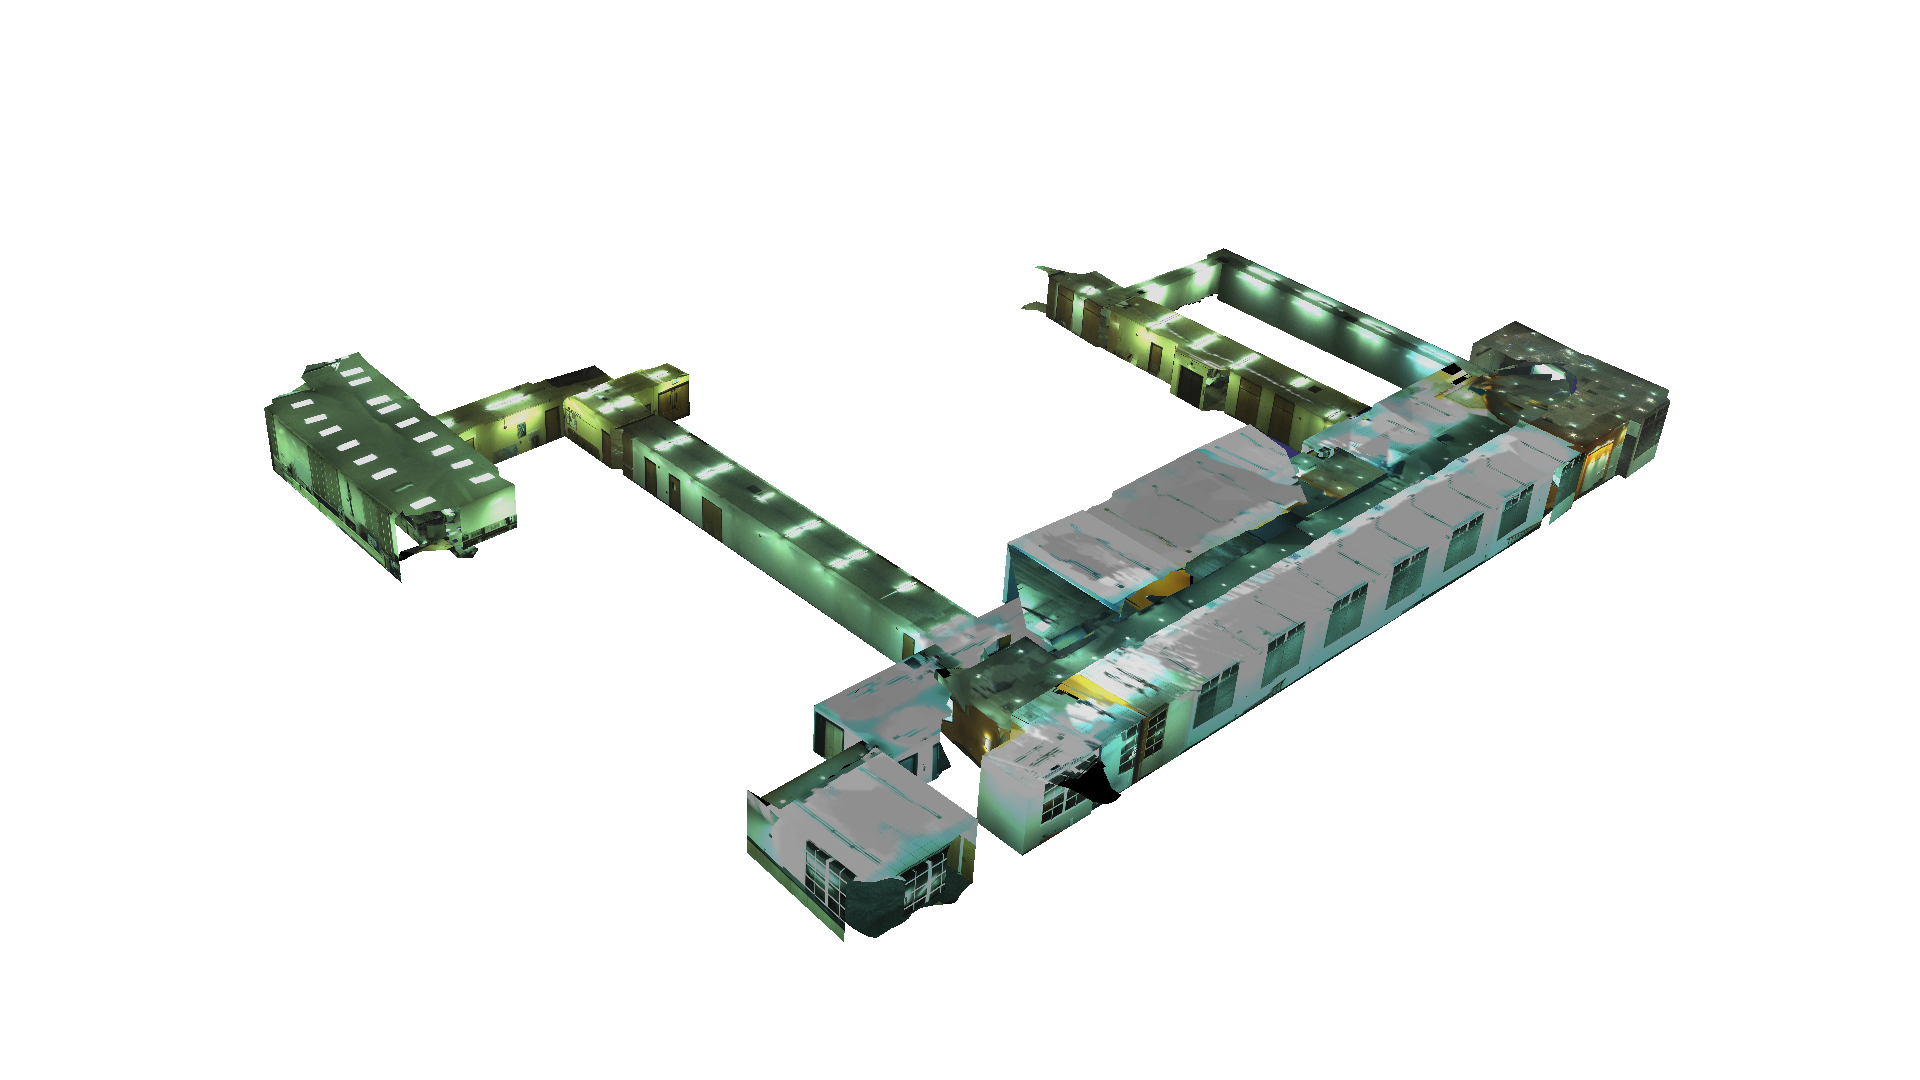
\includegraphics[width=2.2in,height=1.5in]{results_swarm_3_v.png}
  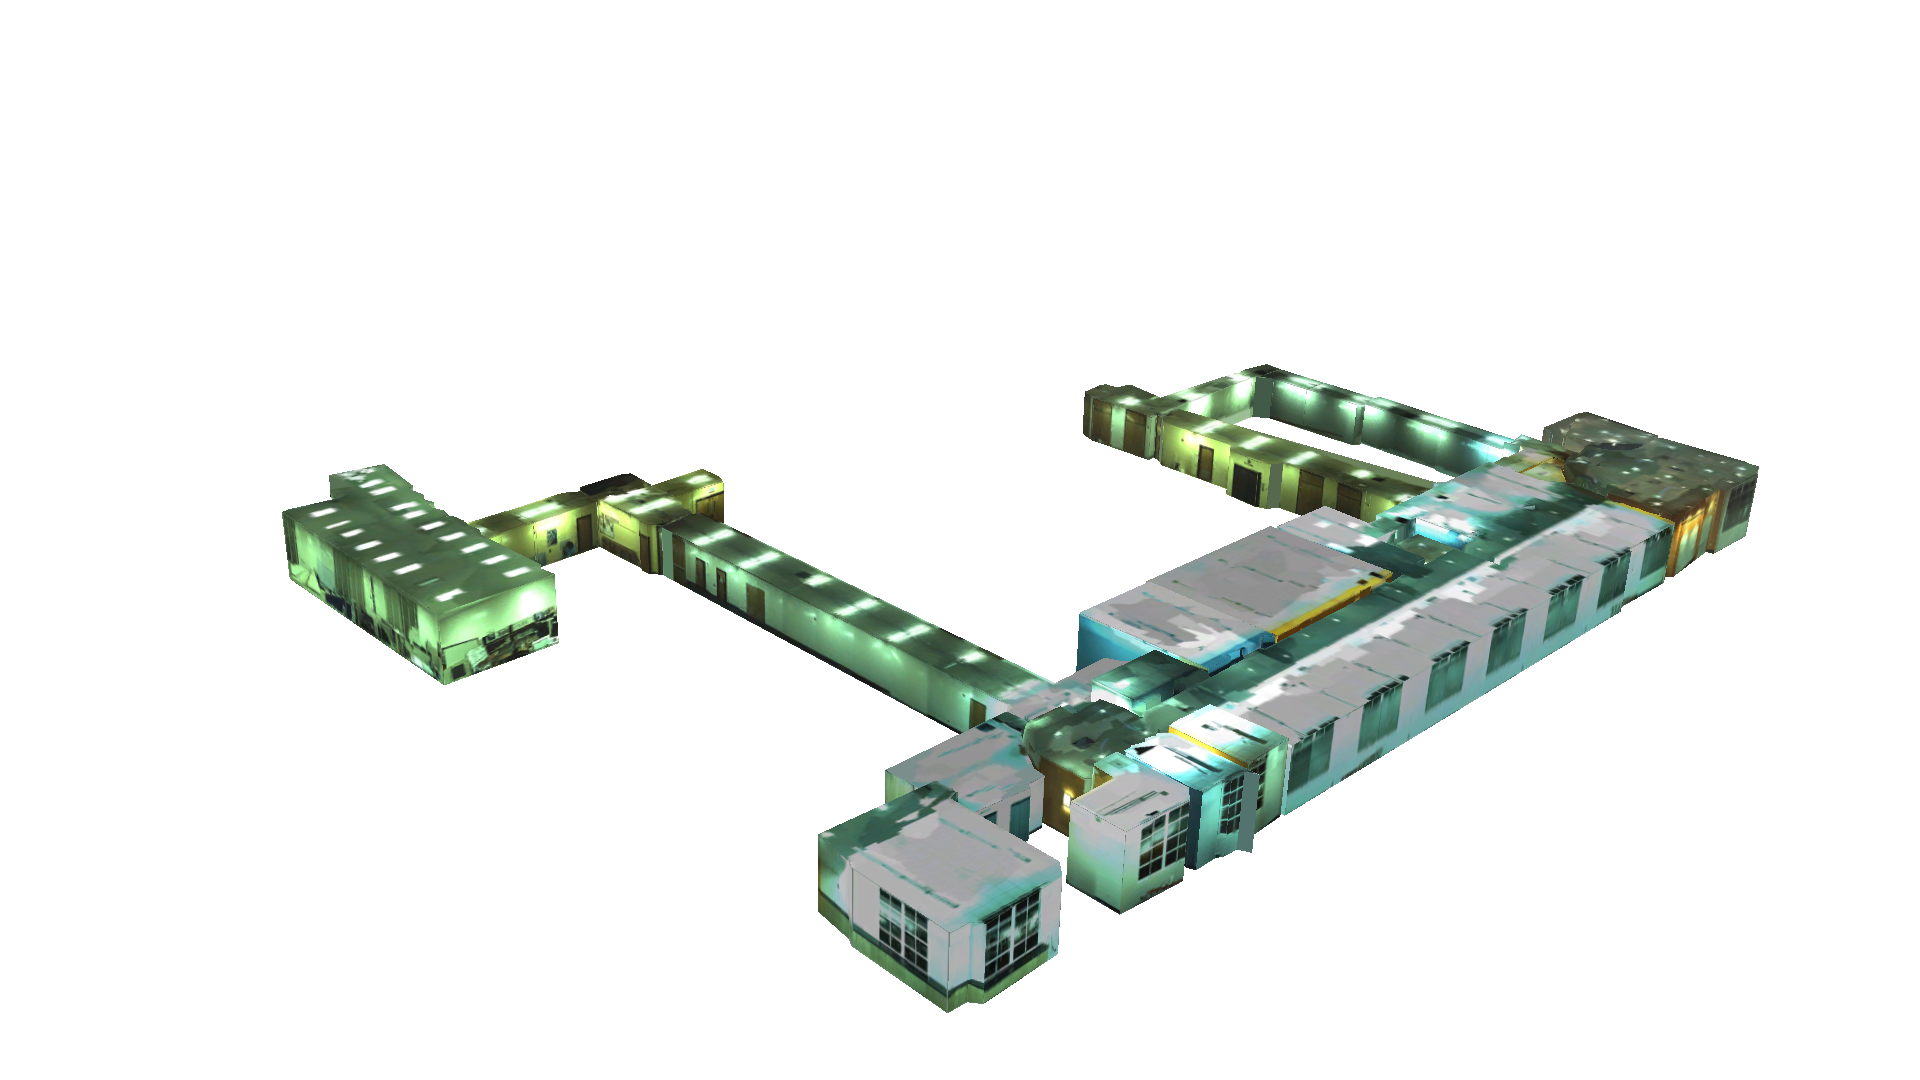
\includegraphics[width=2.2in,height=1.5in]{results_swarm_3_2d.png}
  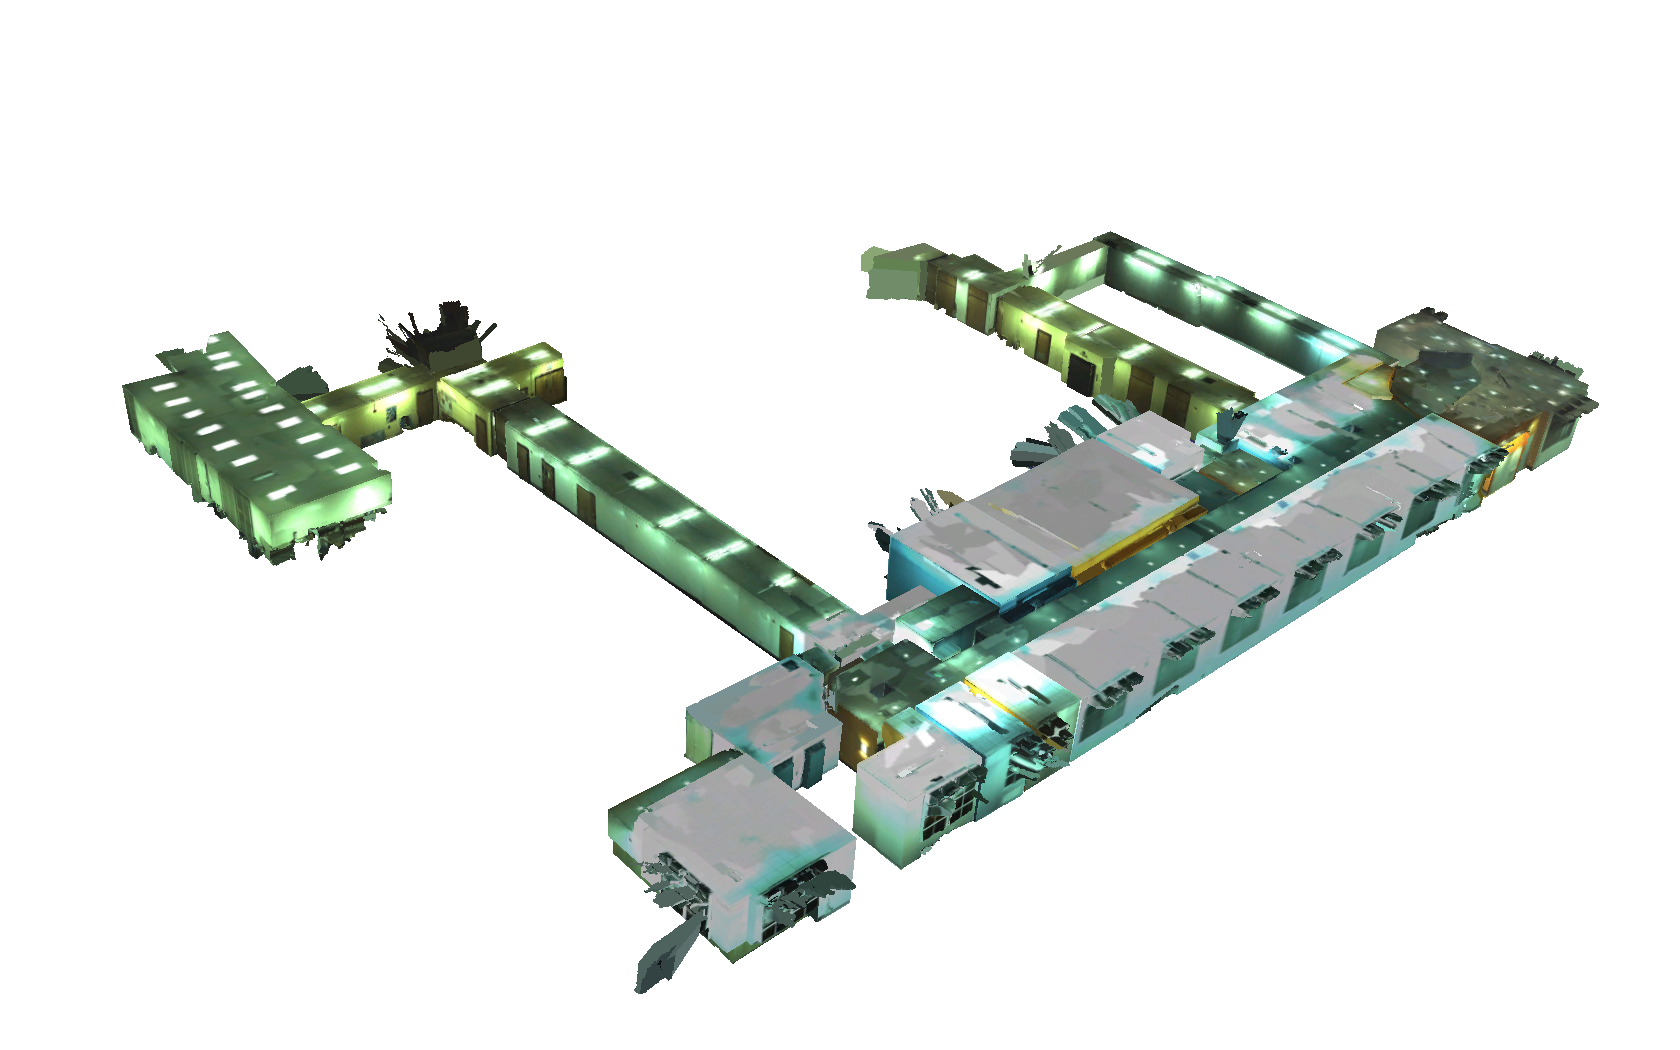
\includegraphics[width=2.2in,height=1.5in]{results_swarm_3_3d.png}\\
  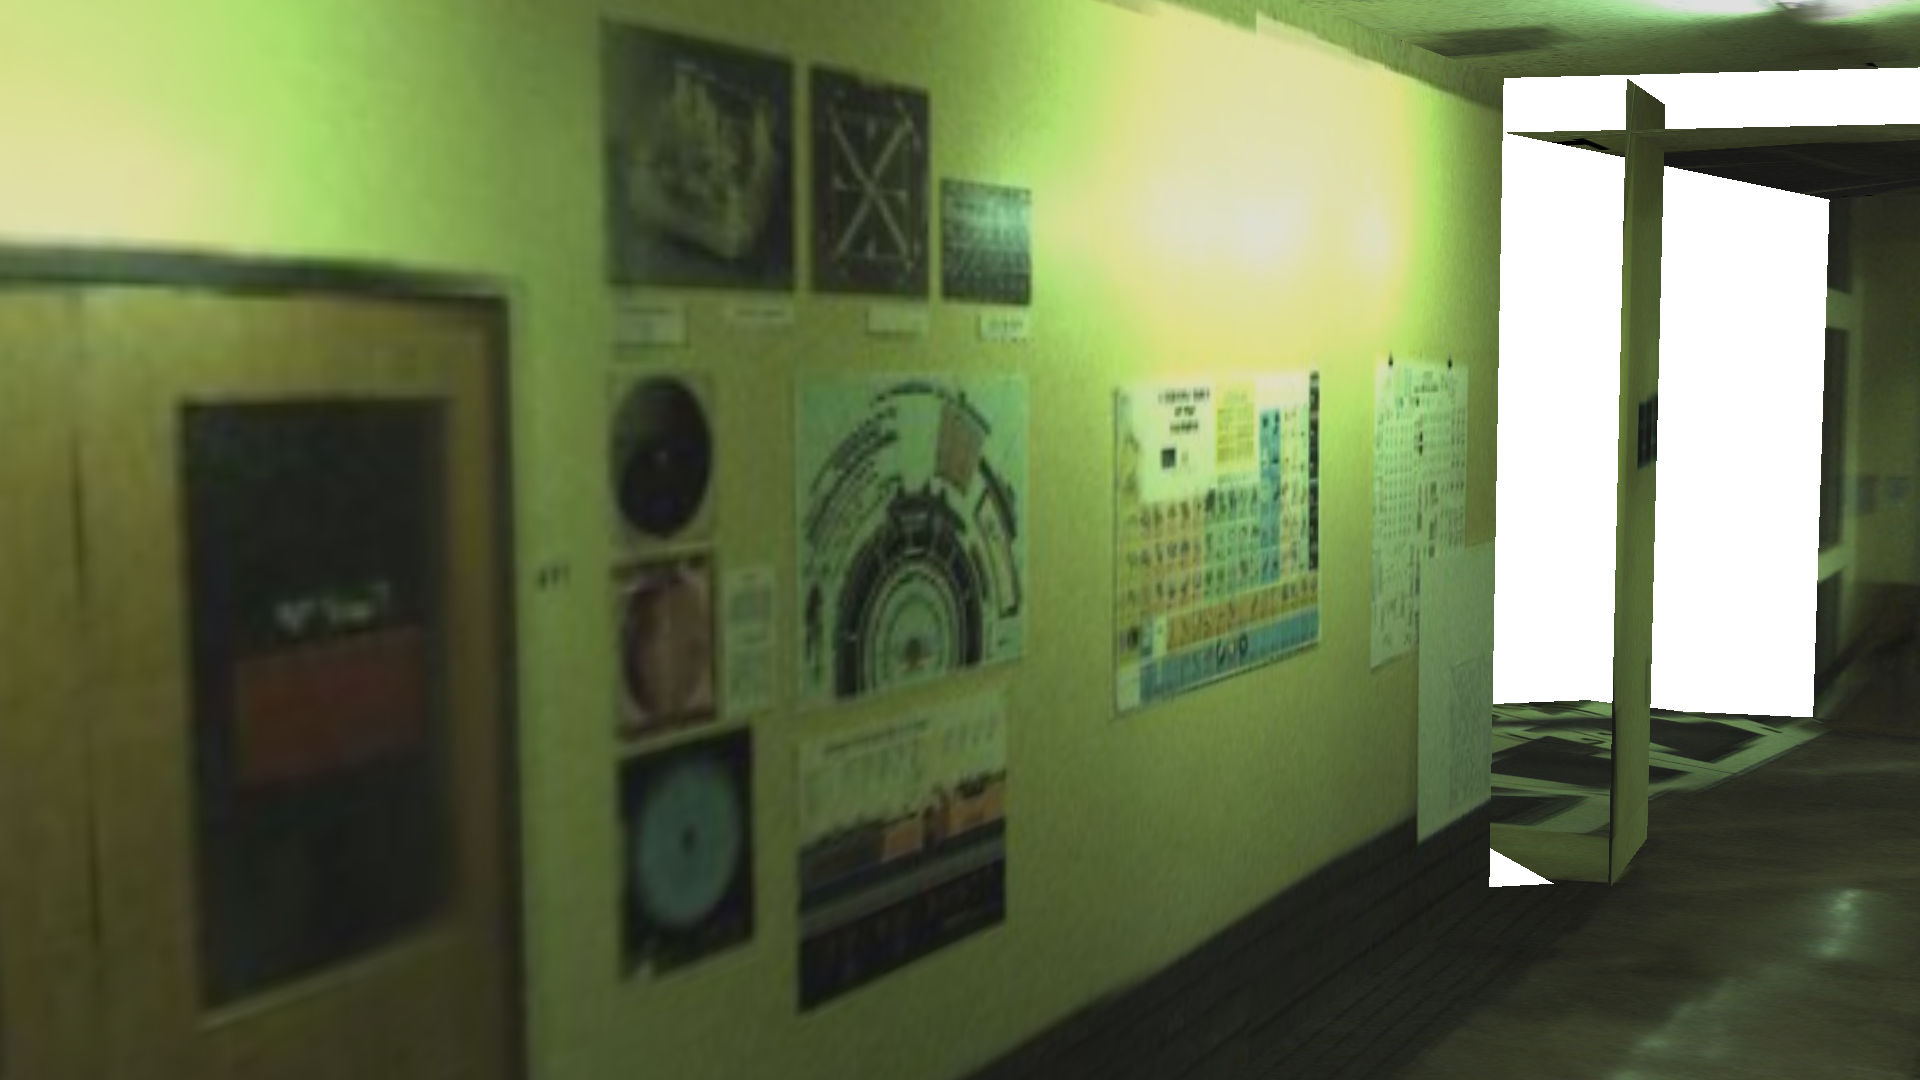
\includegraphics[width=2.1in,height=1.5in]{results_swarm_2_v.png}
  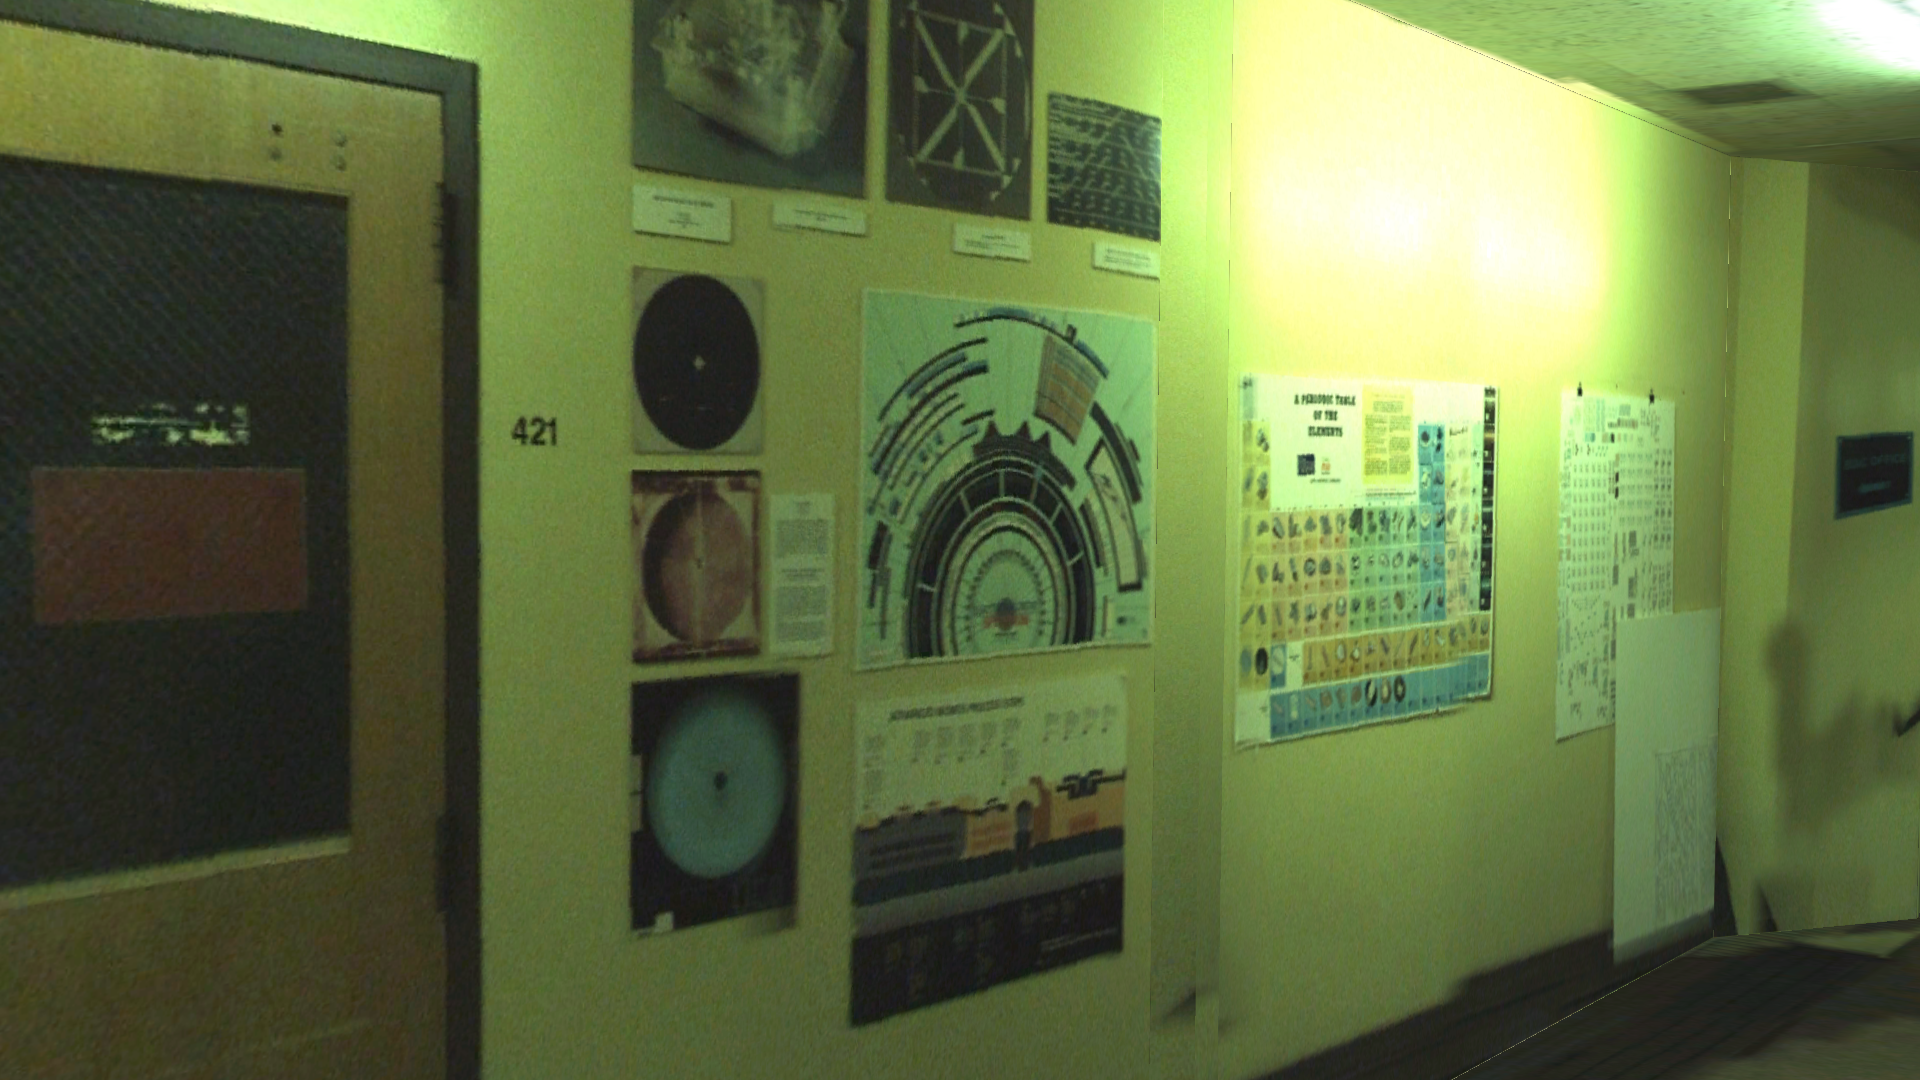
\includegraphics[width=2.1in,height=1.5in]{results_swarm_2_2d.png}
  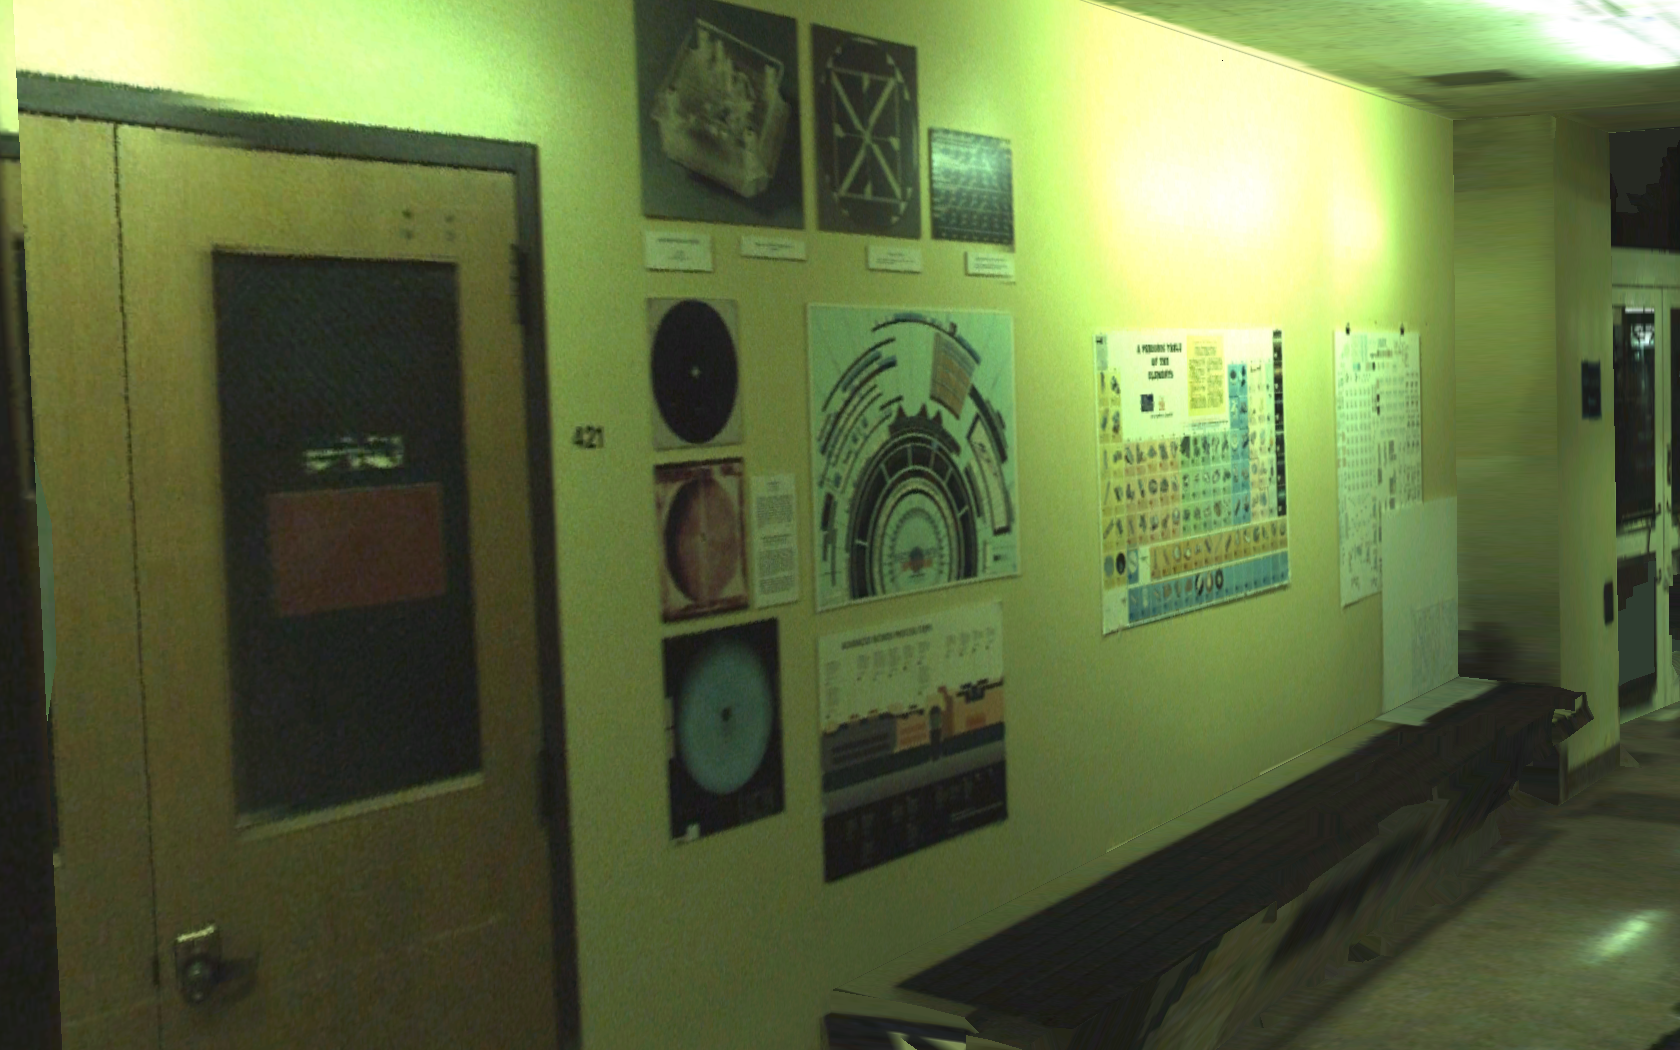
\includegraphics[width=2.1in,height=1.5in]{results_swarm_2_3d.png}\\
  \subfloat[][]{
    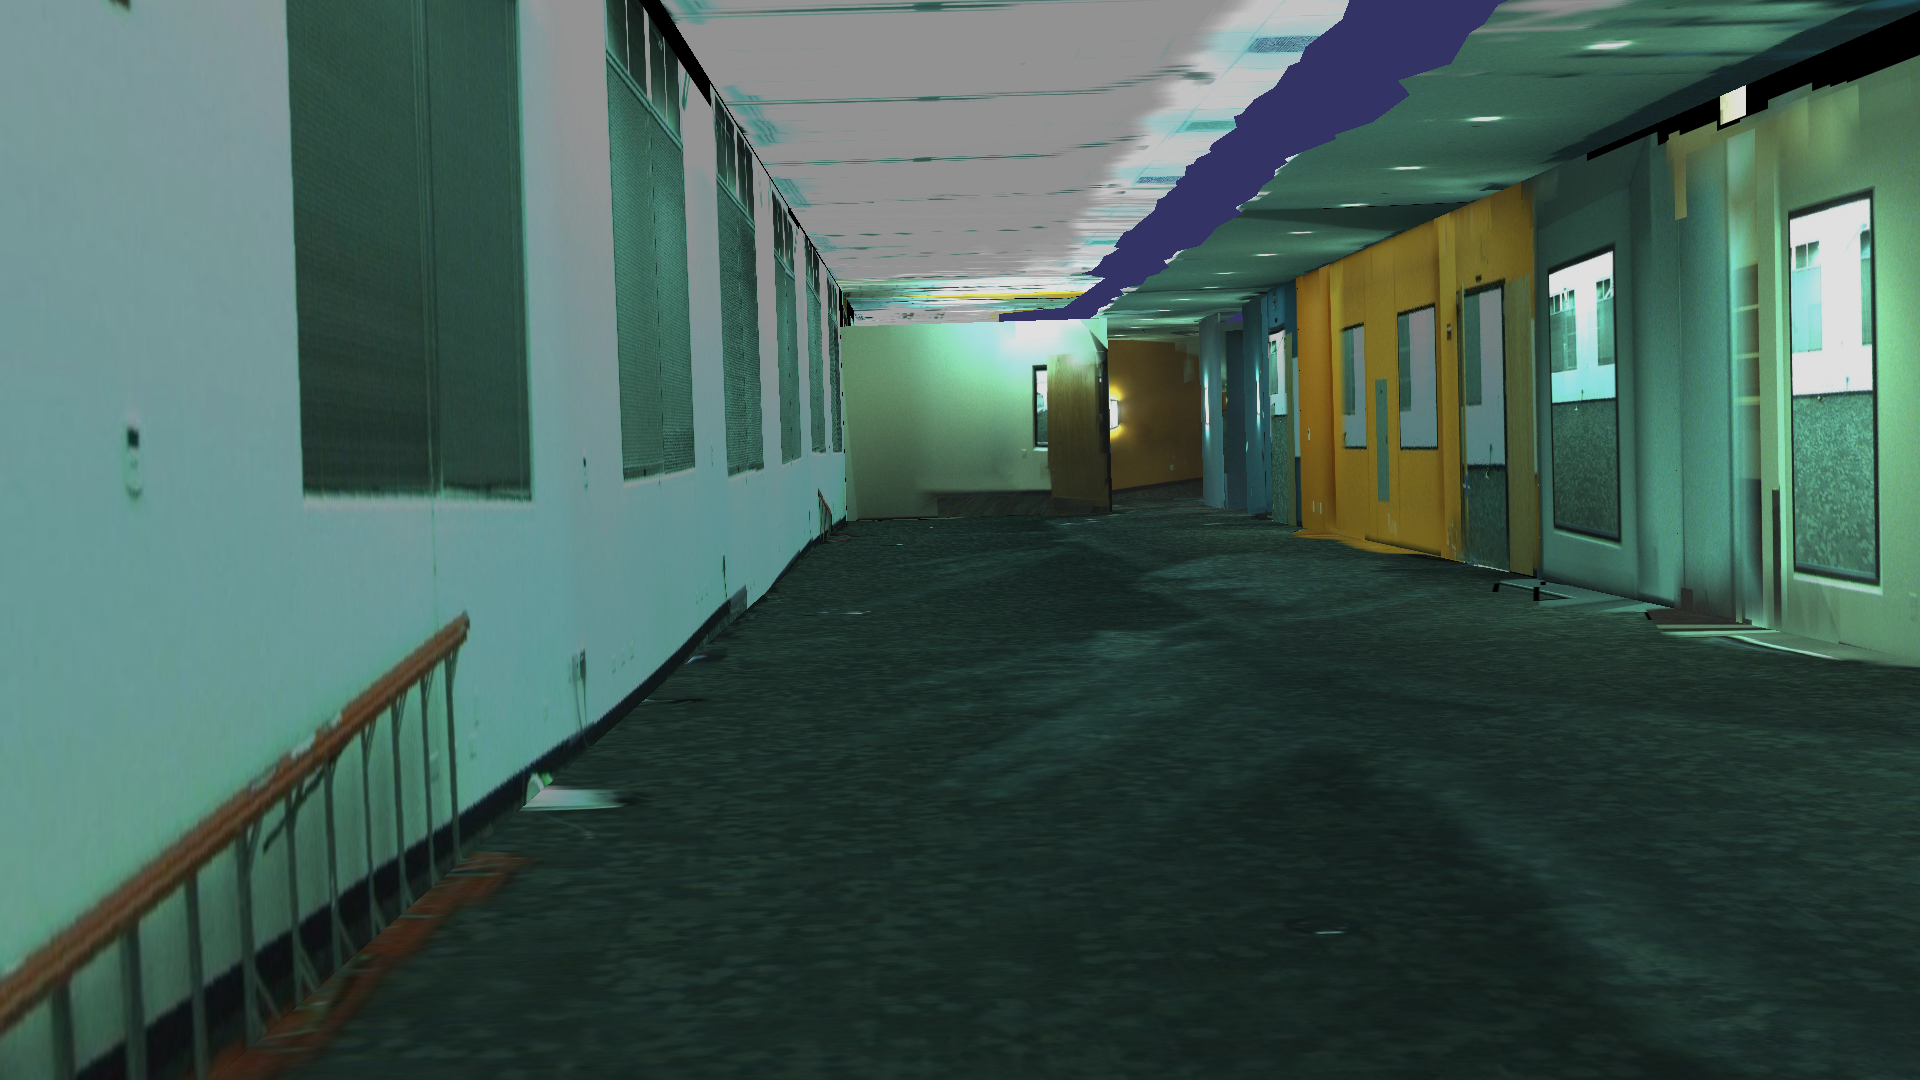
\includegraphics[width=2.1in,height=2in]{results_swarm_5_v.png}
  } \subfloat[][]{
    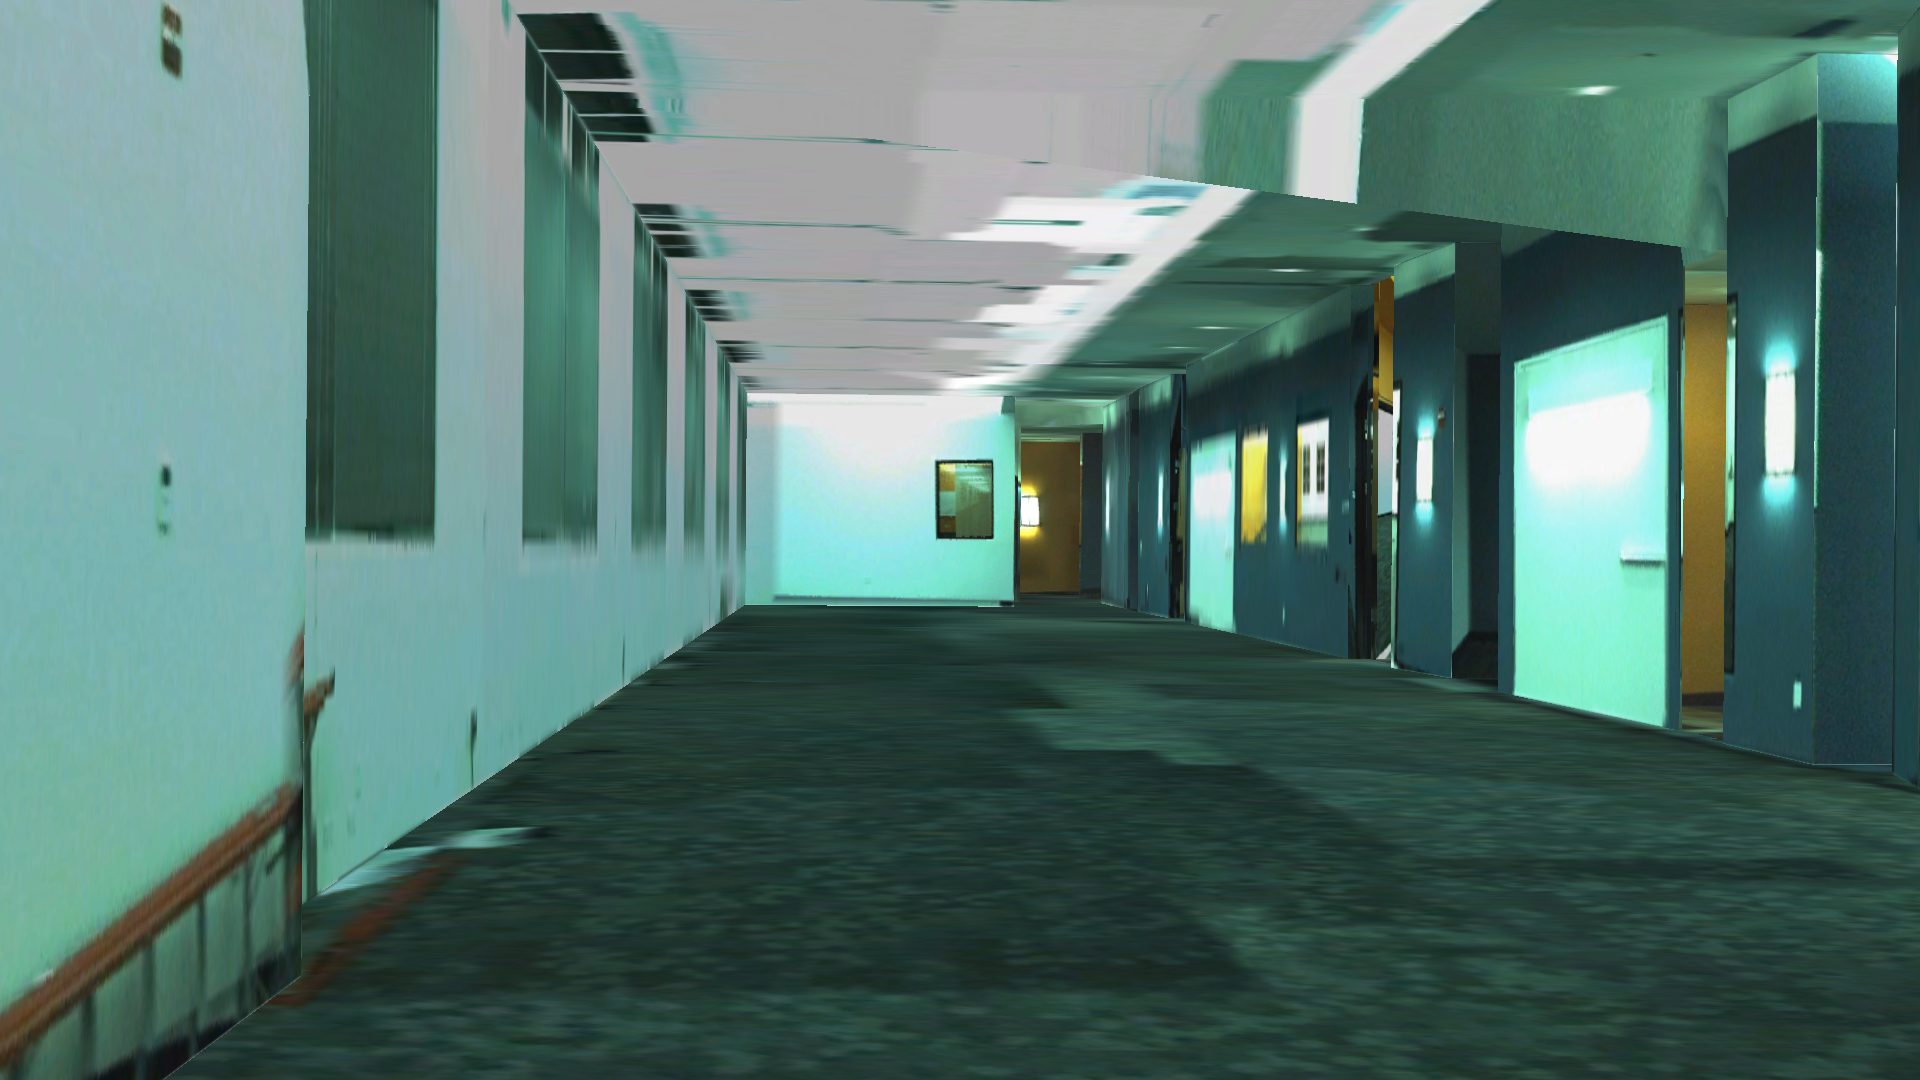
\includegraphics[width=2.1in,height=2in]{results_swarm_5_2d.png}
  } \subfloat[][]{
    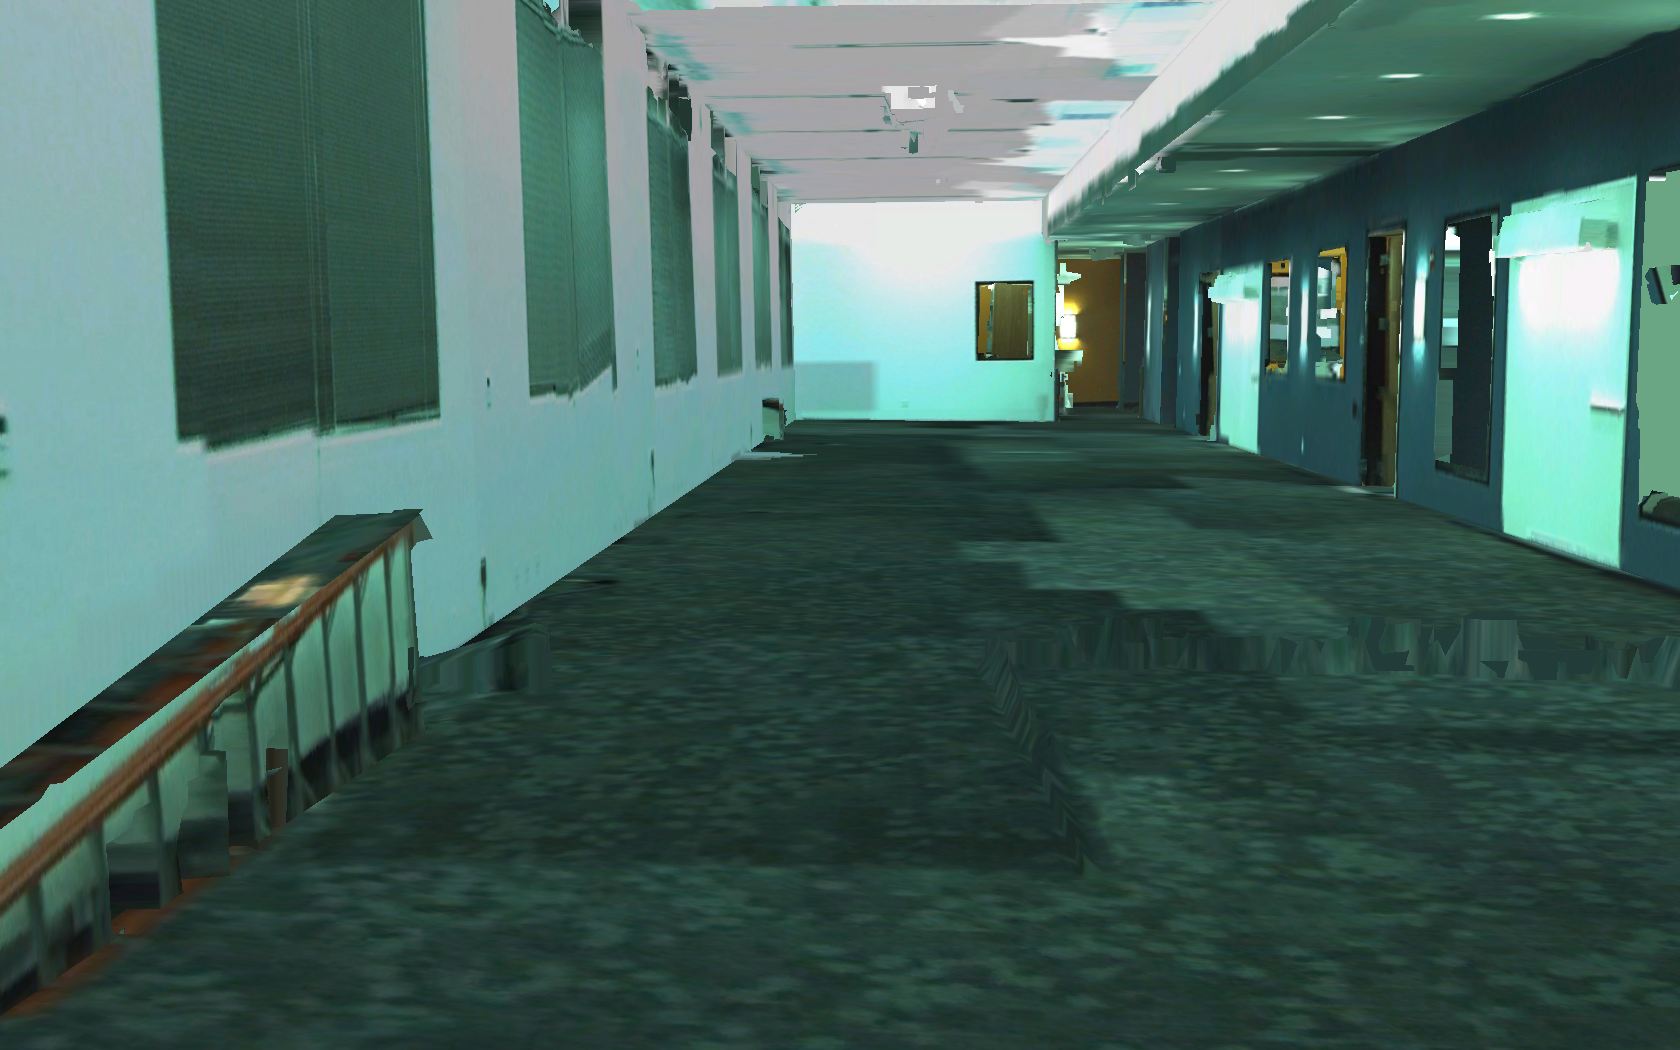
\includegraphics[width=2.1in,height=2in]{results_swarm_5_3d.png}
  }
  \caption{The same indoor environments, as generated using (a) PCA
    plane-fitting, (b) Floor plan extrusion, (c) Voxel carving. The
    first two are low-resolution models, while the third is
    high-resolution. The PCA method is not watertight, and contains
    some holes (white). It also has the lowest level of detail in its
    geometry. The floor plan method is slightly more detailed, and is
    watertight as well. The voxel carving method also produces
    watertight meshes, and reconstructs smaller features, such as the
    bench and the ladder in the lower two images.}
  \label{fig:modelcomparisons}
\end{figure}

Our approach was tested with three different geometry-reconstruction
methods, a PCA-based plane-fitting method \cite{sanchez2012point}, a
floor plan extrusion method \cite{turnerfloorplan}, and a
voxel-carving mesh generation method \cite{turnerwatertight}. The
first two methods generate lower-resolution models, containing only
major walls, ceilings and floors. The third method generates
high-resolution models, and attempts to reconstruct all scanned
objects in the environment. Images illustrating the differences
between the three methods are in Figure \ref{fig:modelcomparisons}

\begin{figure}
  \centering \subfloat[][]{
    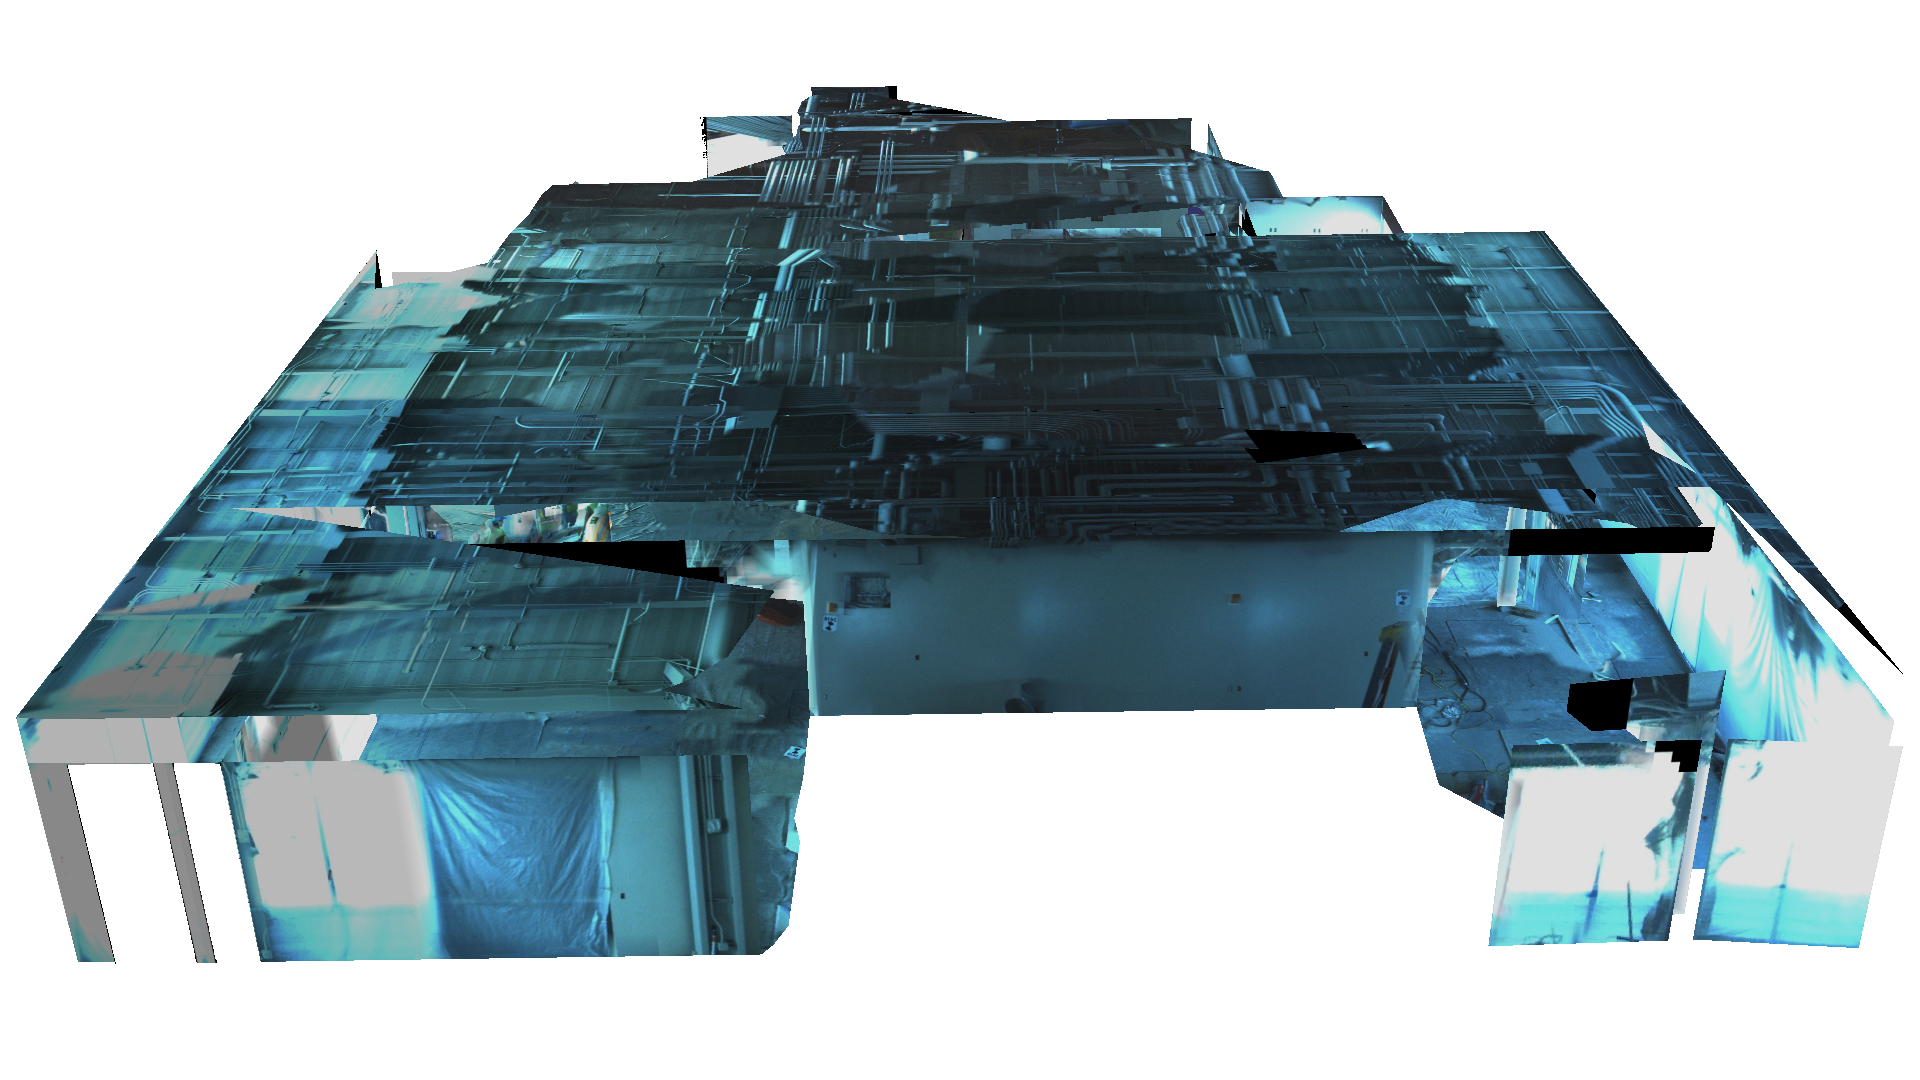
\includegraphics[width=3in]{results_p15_v.png}
  } \subfloat[][]{
    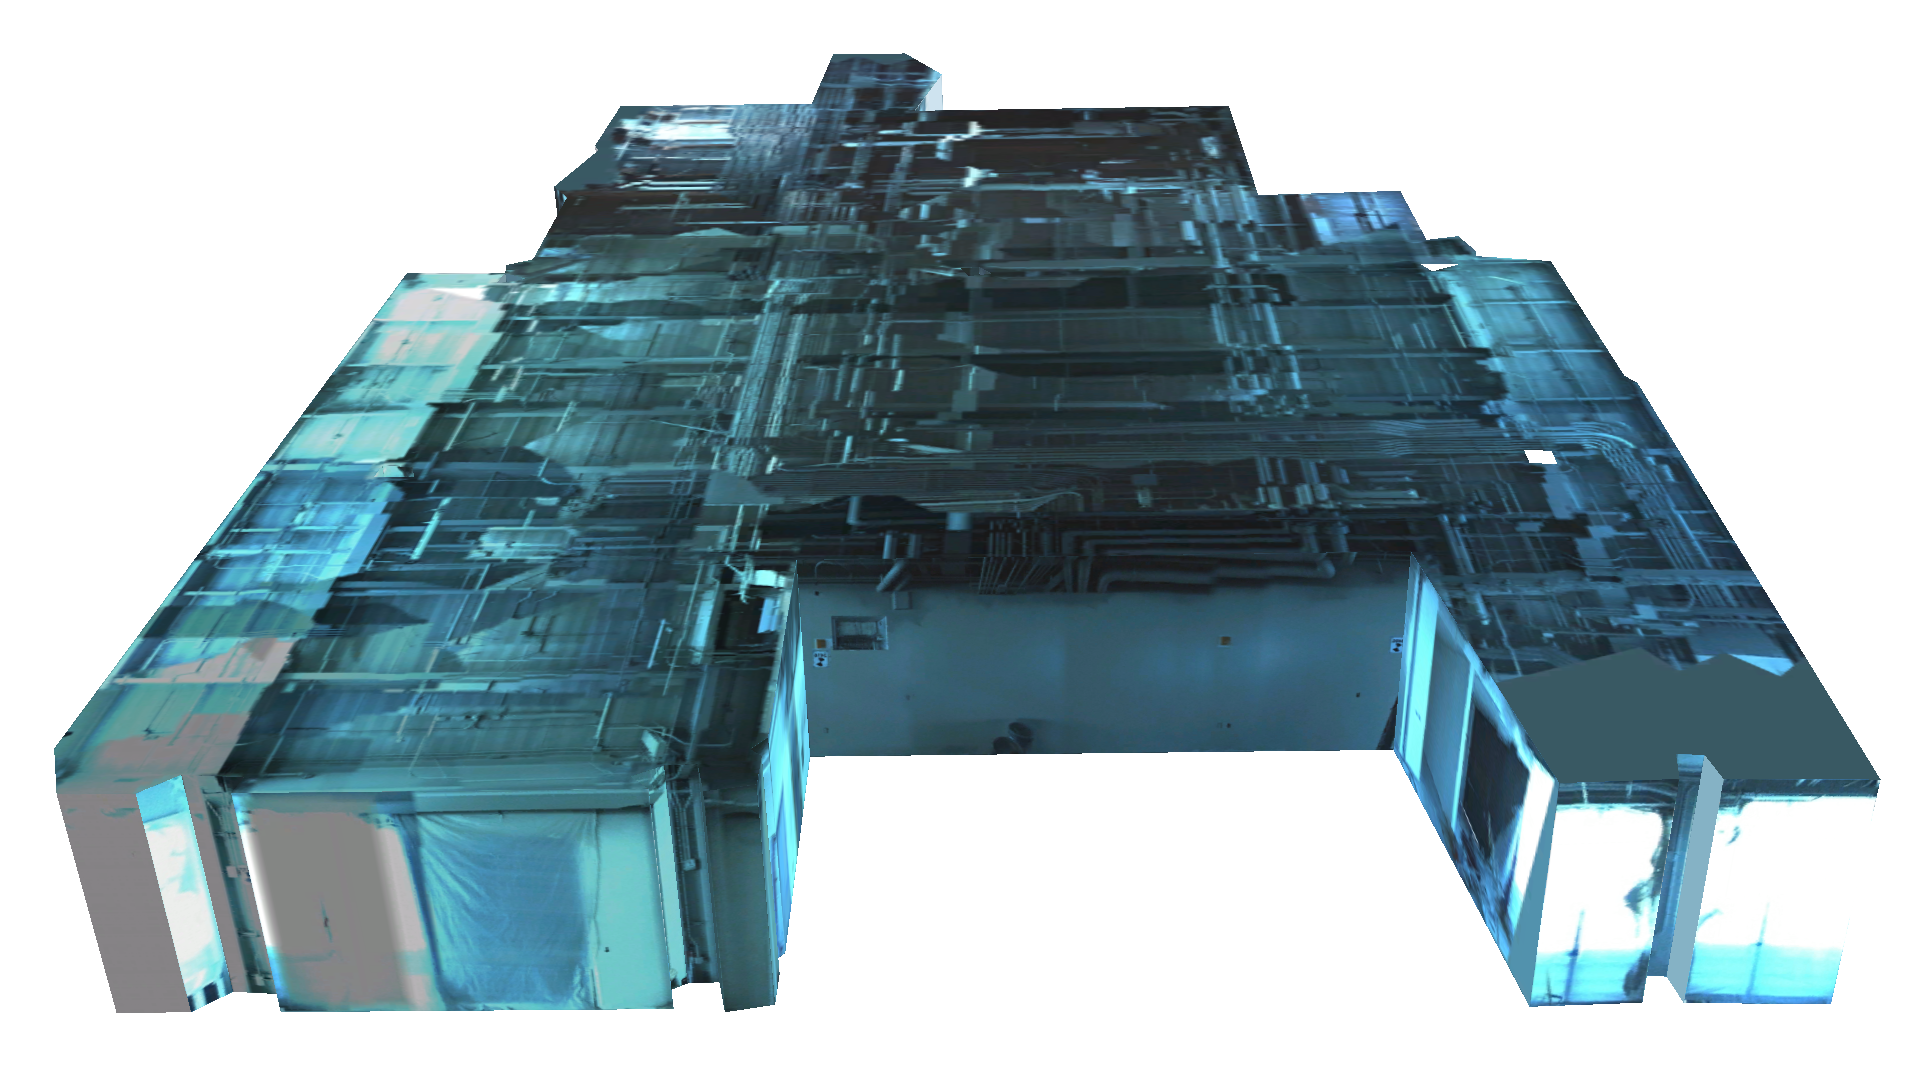
\includegraphics[width=3in]{results_p15_2d.png}
  }
  \caption{(a) A model generated by the PCA method with many missing
    surfaces. (b) A watertight model generated by the floor plan
    extrusion method.}
  \label{fig:lowresmodels}
\end{figure}

The PCA and floor plan methods produce models at a similar level of
detail. As visible in Figure \ref{fig:lowresmodels}, the PCA method is
not watertight, while the floor plan method is. As a result, the
PCA-generated model contains holes where surfaces were not adequately
scanned. On the other hand, the watertight floor plan model sometimes
must make assumptions about the location of surfaces that were not
adequately scanned, in order to maintain watertightness. Because
buildings generally follow straight lines and right angle corners
however, such assumptions tend to be correct. Additionally, the
floor-plan method is generally superior at reconstructing smaller
surfaces, such as small walls, or to approximate curved surfaces,
while the PCA method only fits large planes, and fails in both
cases. As a result, the floor-plan method usually produces more
visually pleasing low-resolution models, and is the method of choice
for generating textured low-resolution models.

\begin{figure}
  \centering
  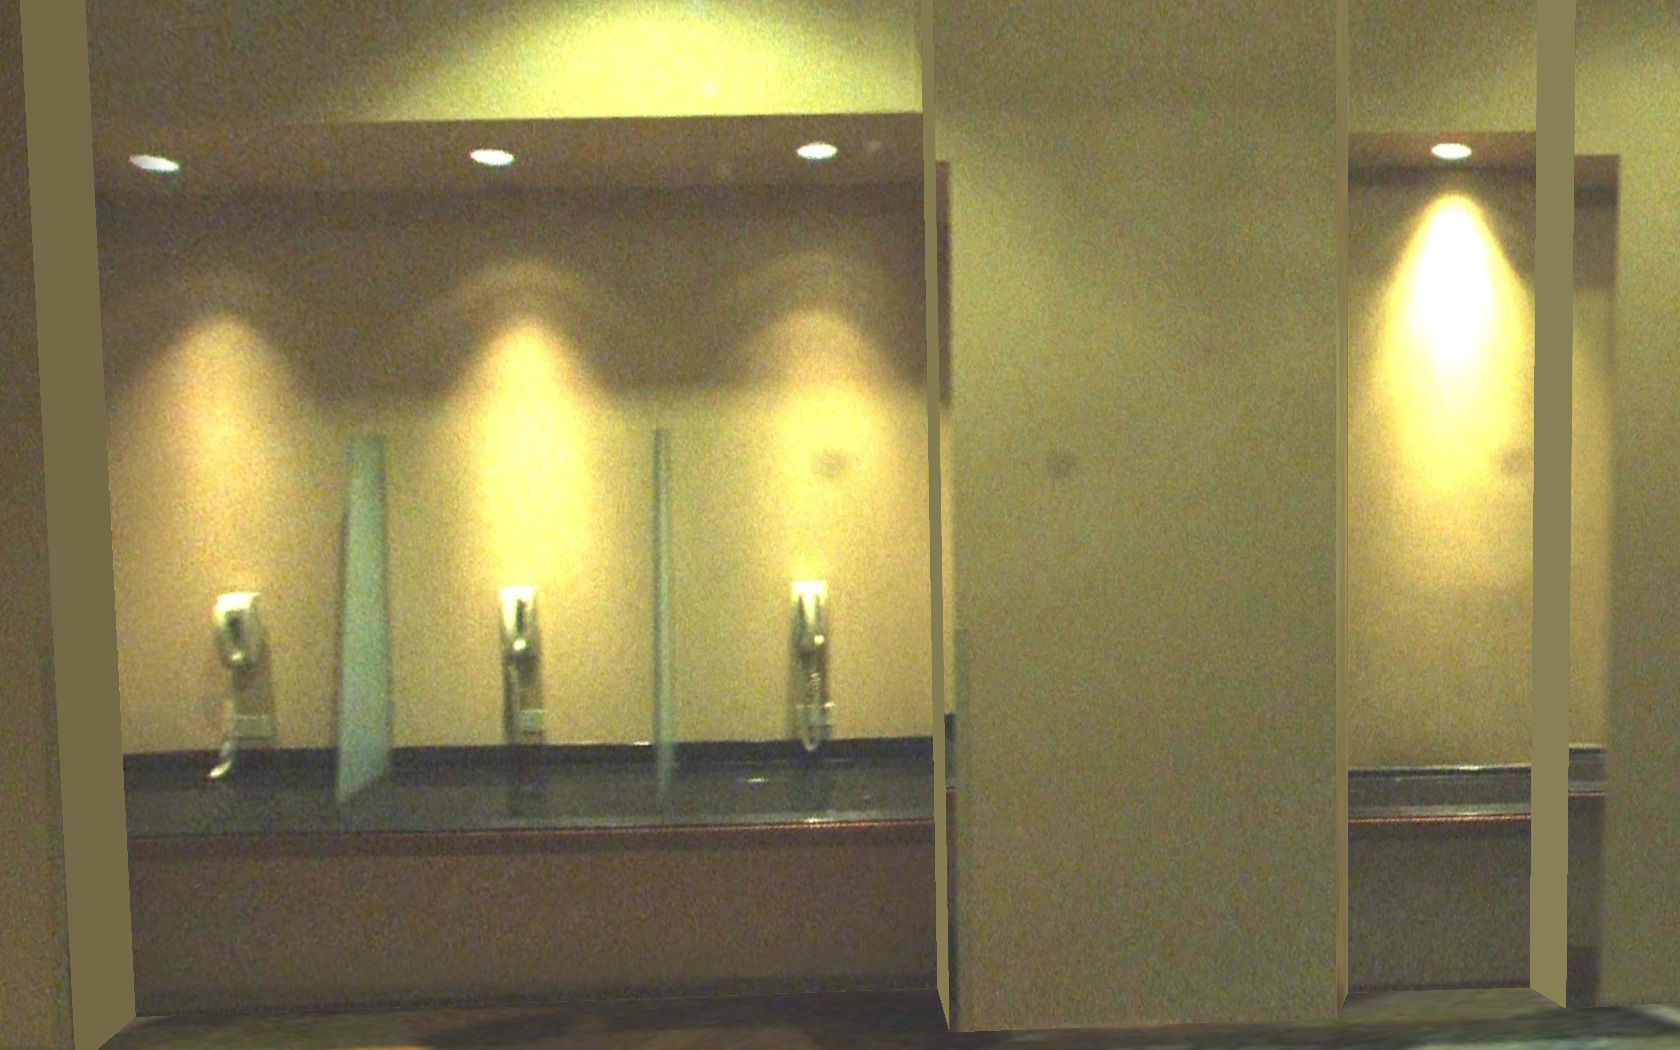
\includegraphics[width=3.1in]{results_houston_1_2d.png}
  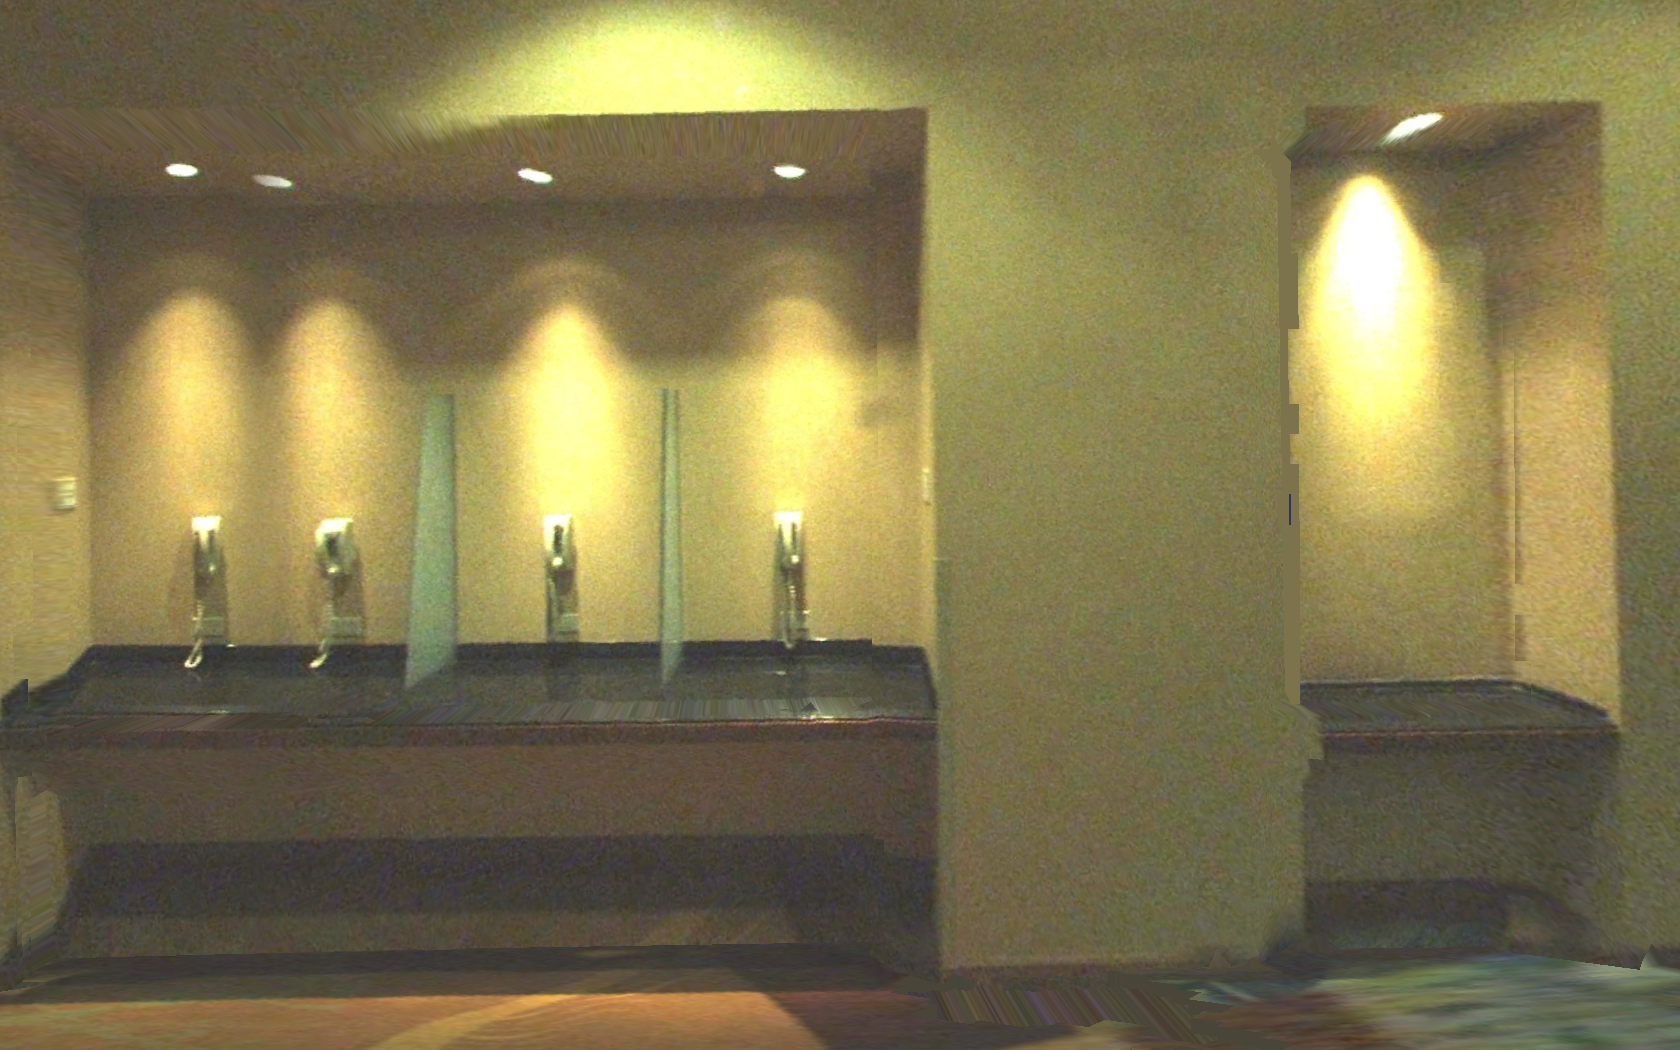
\includegraphics[width=3.1in]{results_houston_1_3d.png}\\
  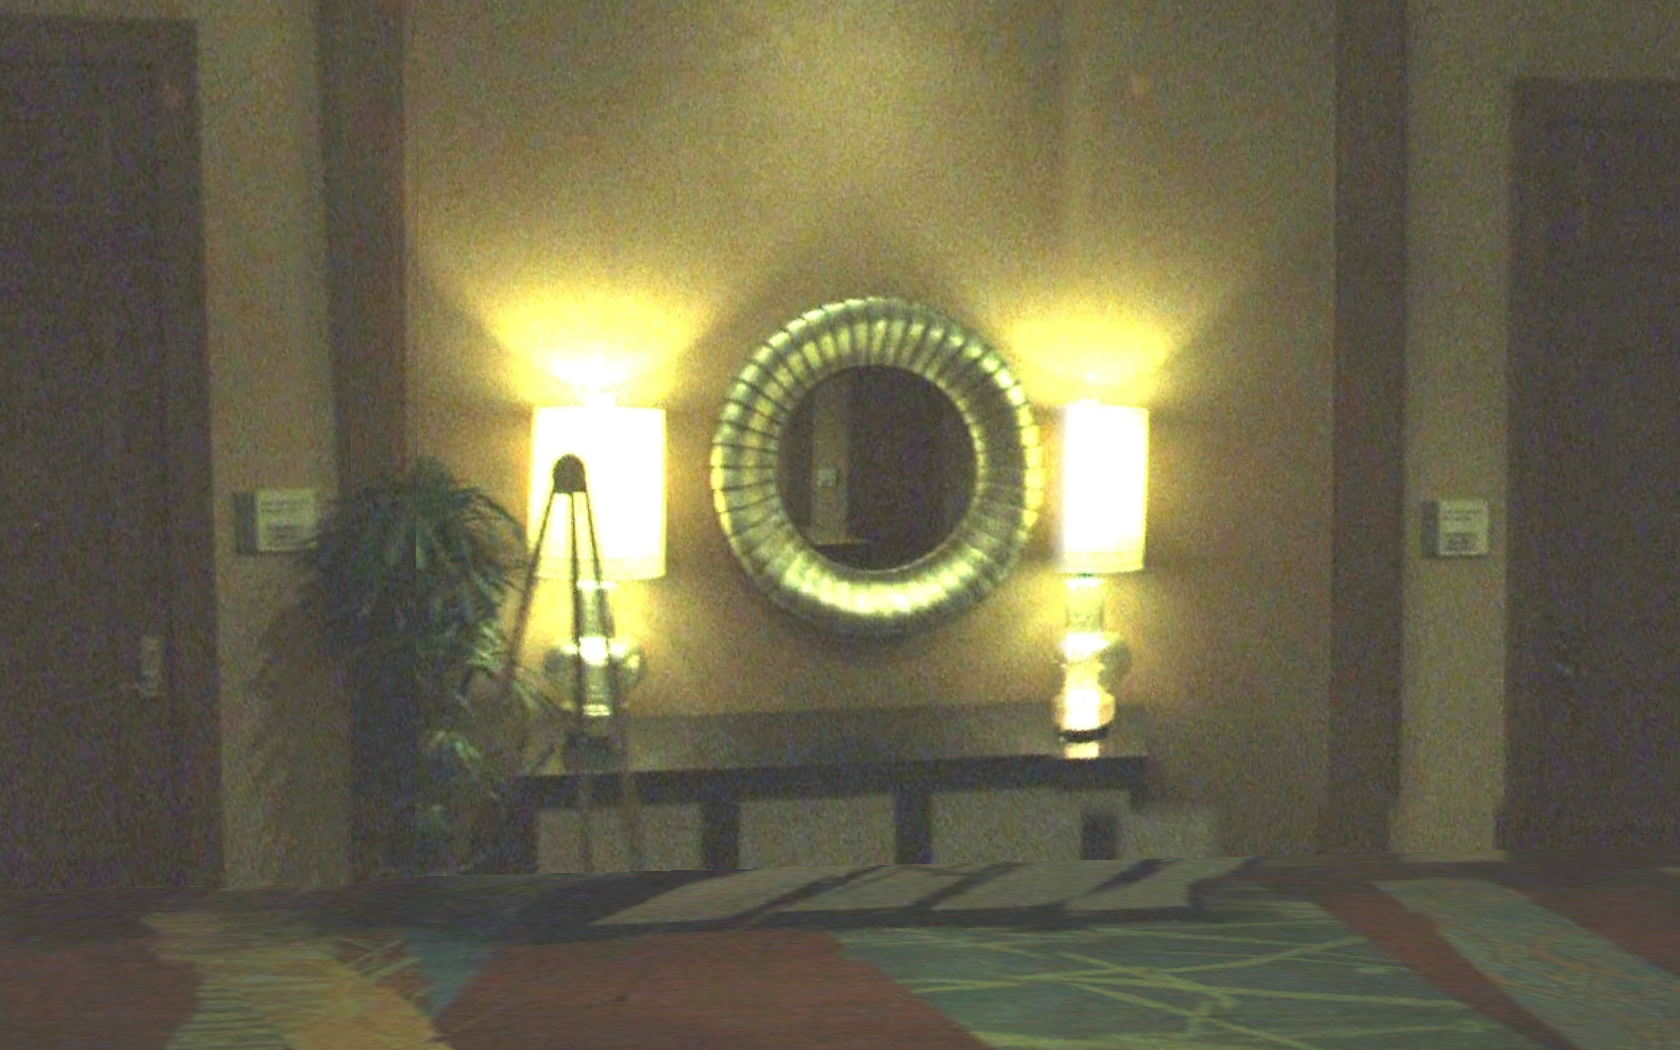
\includegraphics[width=3.1in]{results_houston_2_2d.png}
  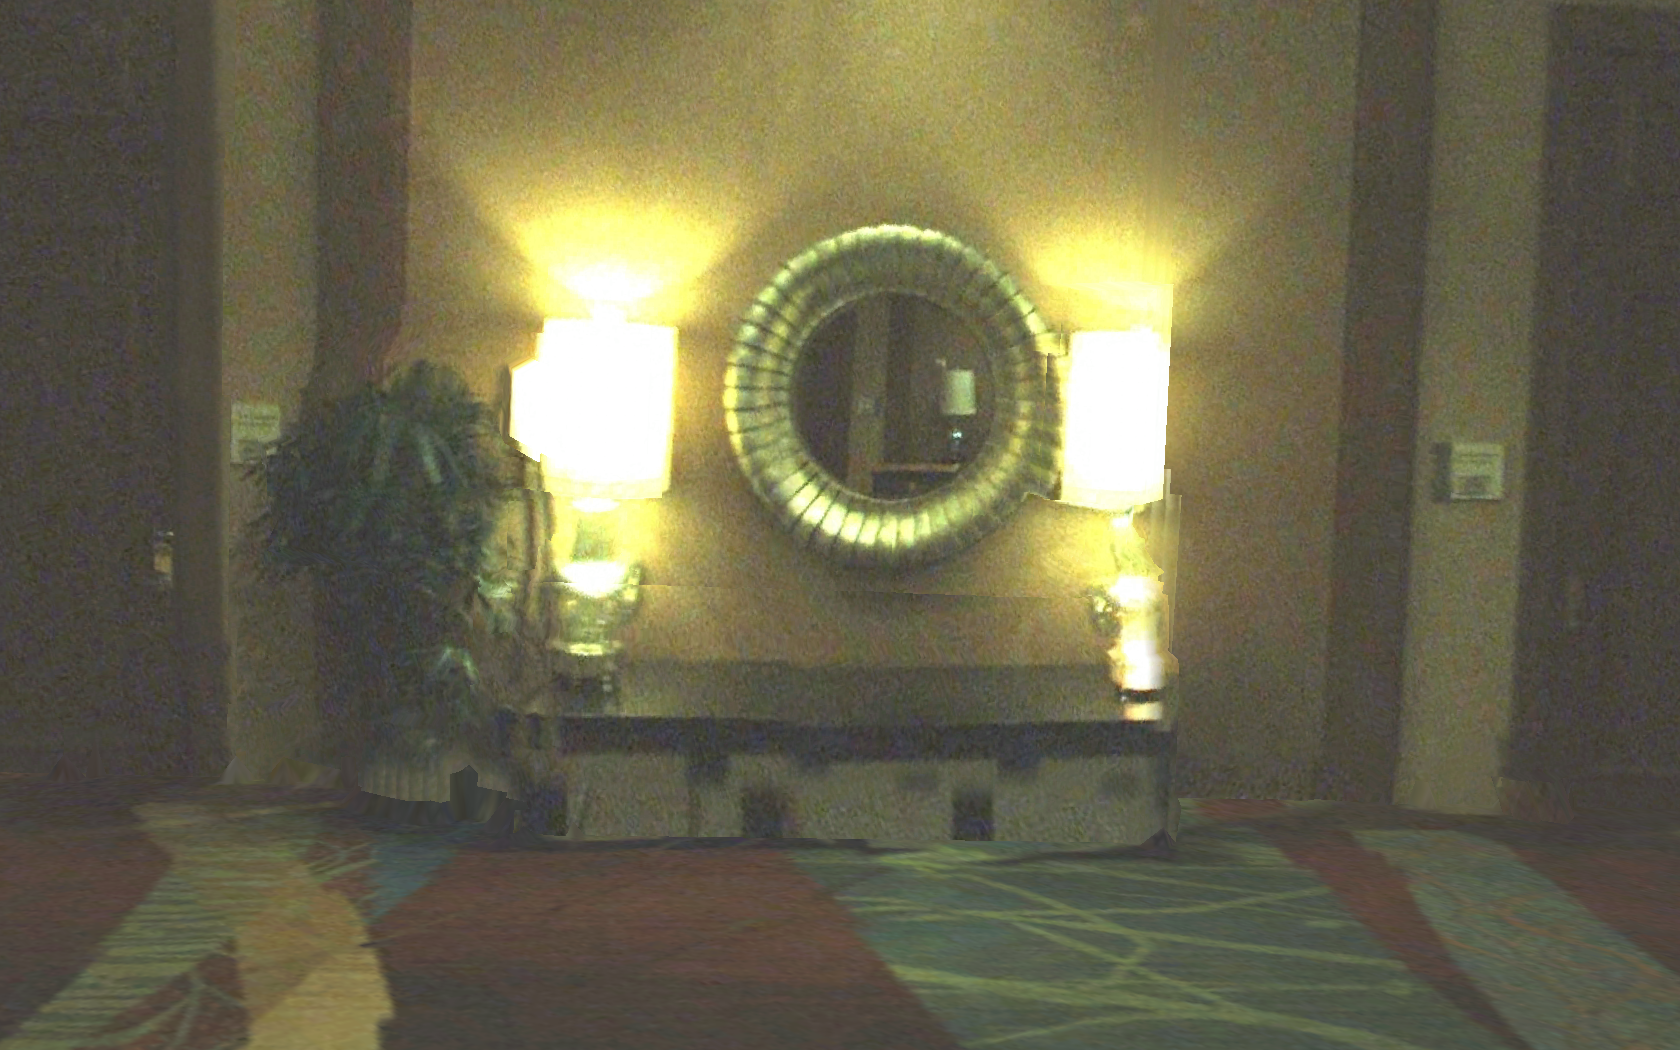
\includegraphics[width=3.1in]{results_houston_2_3d.png}\\
  \subfloat[][]{
    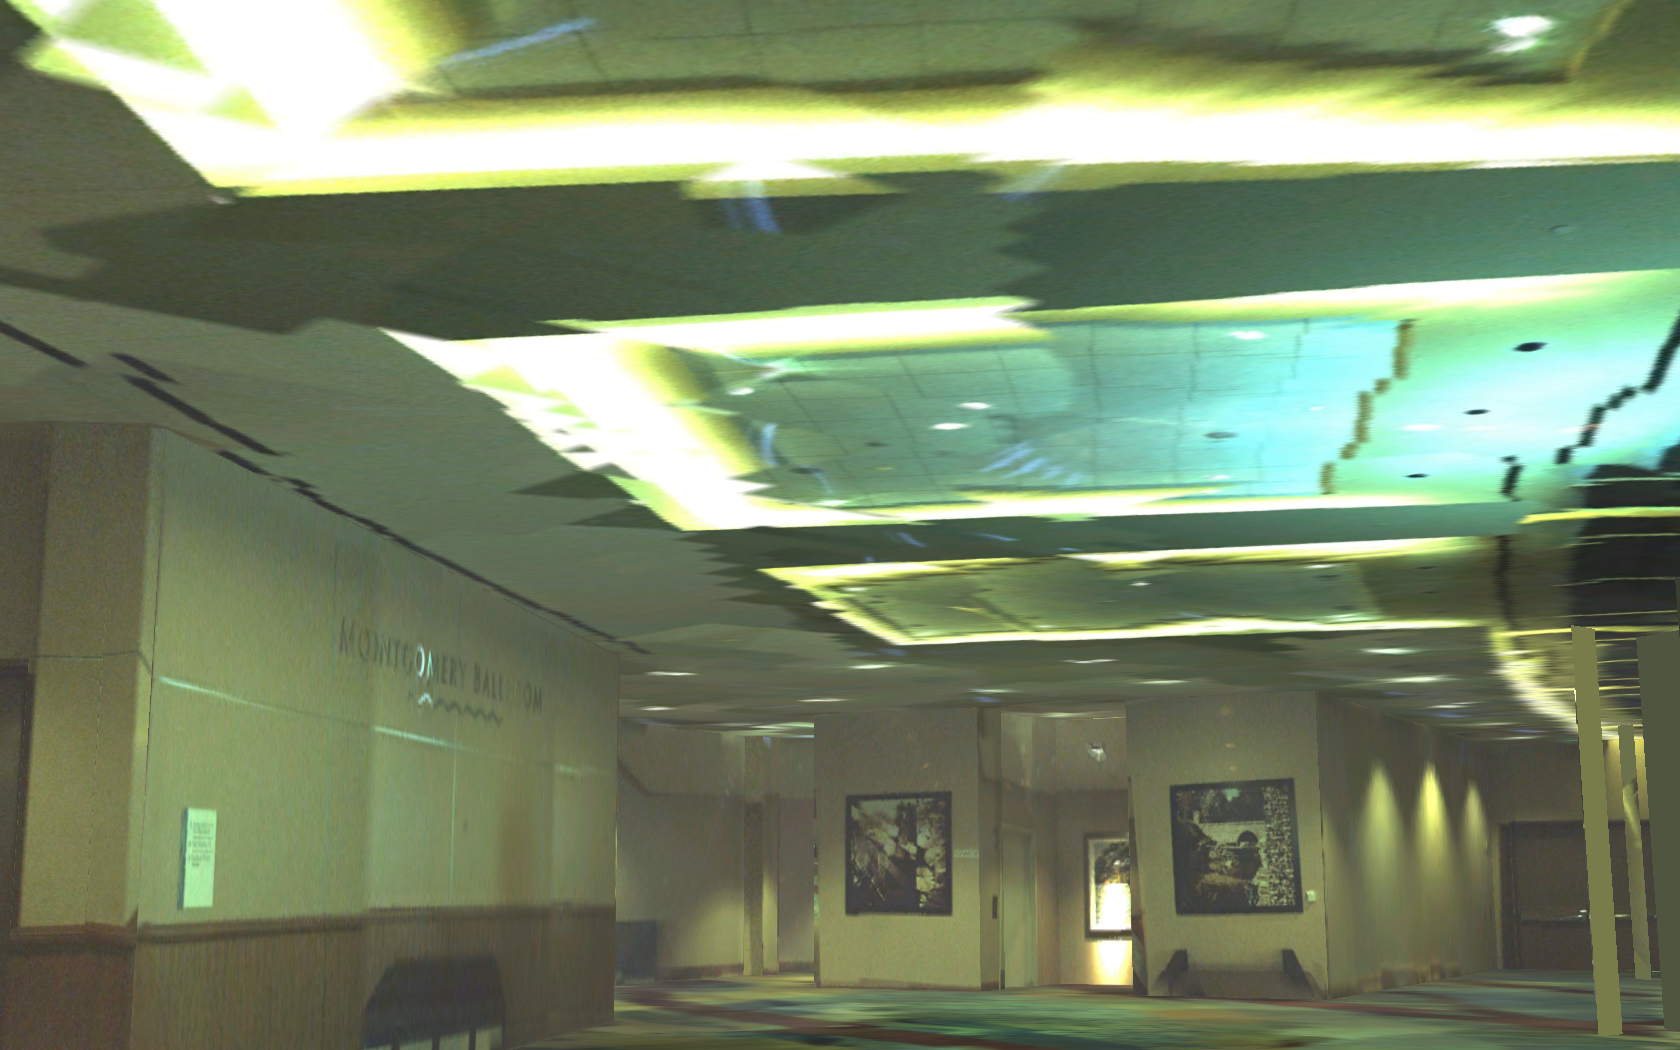
\includegraphics[width=3.1in]{results_houston_3_2d.png}
  } \subfloat[][]{
    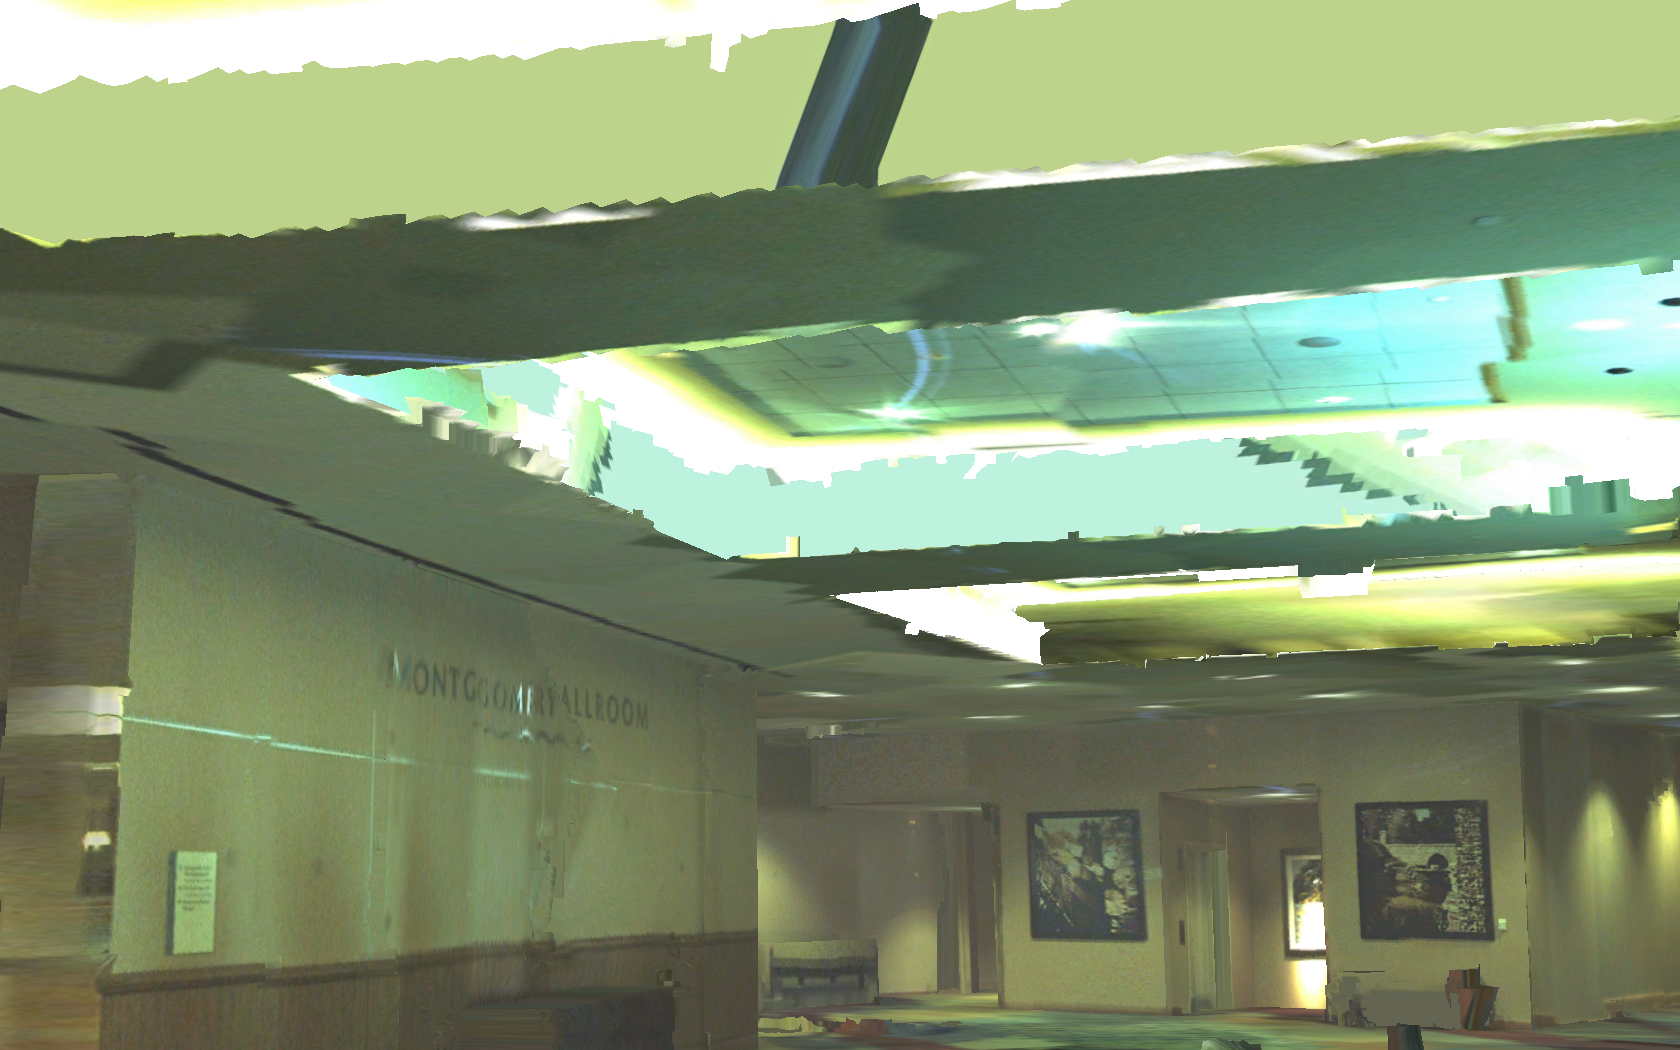
\includegraphics[width=3.1in]{results_houston_3_3d.png}
  }
  \caption{(a) A model generated by the low-resolution floor plan
    method. (b) A model generated by the high-resolution voxel-carving
    method. The high-resolution model contains far more surface
    detail, such as in the ceiling indentations or the benches on the
    ground. In terms of producing a realistic visualization however,
    the low-resolution model performs very similarly to the
    high-resolution model.}
  \label{fig:2dvs3d}
\end{figure}

High-resolution models, as generated by the voxel-carving method, can
produce more accurate reconstructions of environment geometry. With
such models, region partitioning, as described in Section
\ref{sec:geometryPartitioning}, plays an important factor in the
quality of generated textures. If regions are small, boundaries
between adjacent textures become visible, and since each region is
processed independently, image alignment procedures are performed
across smaller areas. If regions are large, then the difference
between the 3D surface geometry and the approximated 2D texturing
surface become large as well, introducing greater texture projection
error. Additionally, in areas where pose error or surface
reconstruction error is high, 3D objects in images do not get
accurately projected onto their modeled counterparts. While large
objects can be aligned to geometry via the methods in Section
\ref{sec:geometryAlignment}, smaller objects such as plants or
computers are difficult to line up to geometry references. While the
compositing techniques is Section \ref{sec:imageCompositing} can
ensure that textures for small objects appear seamless, such textures
may not map accurately upon their corresponding geometry, leading to
visually obvious discrepancies in the textured model. Figure
\ref{fig:2dvs3d} contains textured examples from the low-resolution
floor plan approach alongside examples from the high-resolution
voxel-carving approach. As evident in the image comparisons, the 3D
models may be more accurate, but the 2D models often allow for a
cleaner visualization, with larger regions over which images are
successfully composited together.

As visible in Figure \ref{fig:2dvs3d} and other images in this
section, 2D models using the floor plan approach are generally
preferred, as they provide enough detail in geometry to reconstruct
the basic layout of an environment, while textures can be used to
visualize smaller details. On the other hand, for applications where
furniture and smaller interior details are important, applying
textures to the 3D voxel-carved models provides useful image-based
context for visualizing indoor areas. Further examples of
texture-mapped models are contained at the end of this
document. Figure \ref{fig:indivPlanes} contains textured surfaces
alone. Figures \ref{fig:victor1}-\ref{fig:e2d4} contain interior and
exterior views of low-resolution models. Figures
\ref{fig:e3d1}-\ref{fig:e3d3} contain interior and exterior views of
high-resolution models.


\subsection{Runtime}
As mentioned earlier, our approach is quite efficient. The top wall in
Figure \ref{fig:indivPlanes}(a) was generated with 7543 $\times$ 776
pixels, and spans a 40-meter long wall. Given 41000 input images in
the entire dataset, a 2.8GHz dual-core consumer-grade laptop takes
under a second to choose 36 candidate images, followed by a minute to
perform image projections, image alignment, and the shortest path
texturing method. The tile-caching approach takes roughly comparable
time, and over 75\% of the time for either method is spent on
calculating image projections, which are cached over multiple runs,
and also could be performed as a preprocessing step instead. While not
real-time, the process is capable of generating fast updates after
changes in various parameters or modifications to input data, and if
integrated directly into a 3D modeling system, could provide quick
visual feedback as data is collected.


\subsection{Visualization}
Our full models consist of an input model file, generated textures,
and a mapping of image points to 3D model vertices. The textured
models shown throughout this thesis range from 20 MB in size to over
400 MB in a compressed format, with textures of sizes over 500
megapixels. These models are visualized using the OpenSceneGraph
toolkit \cite{openscenegraph}, which allows for export to many common
model formats, as well as interactive visualization, even in web
browsers or mobile devices.

\section{Conclusion}
\label{sec:conclusion}

In this thesis, we have developed an approach to texture mapping
models of indoor environments with noisy camera localization data. We
are able to refine image locations based on geometry references and
feature matching, and robustly handle outliers. Using the tile-based
mapping approach, we can texture both large planar features as well as
smaller, more complex surfaces. We also implemented a shortest path
texturing method that produces seamless textures on planes where
multiple head-on images are available. Both of these approaches are
highly modular, and easily tunable for similar systems across multiple
environments.

Our method is likely to fail however in scenarios where 3D error is
large. A logical progression of our approach to resolve camera error
in 3D is to perform matching between image lines and geometry in 3D,
which can be done reasonably efficiently \cite{linebased,
  rectangularstructures}. Using linear features in addition to SIFT
features is also likely to result in improved matches, as indoor
scenes often have long, unbroken lines spanning multiple images
\cite{linearposeestimation}. Finally, the blending procedure is quite
basic, and applying more sophisticated methods of blending,
normalization, as well as image boundary selection would benefit the
final visual quality, and more robustly handle motion-based or
parallax errors.



\begin{figure}
  \centering
  \subfloat[][]{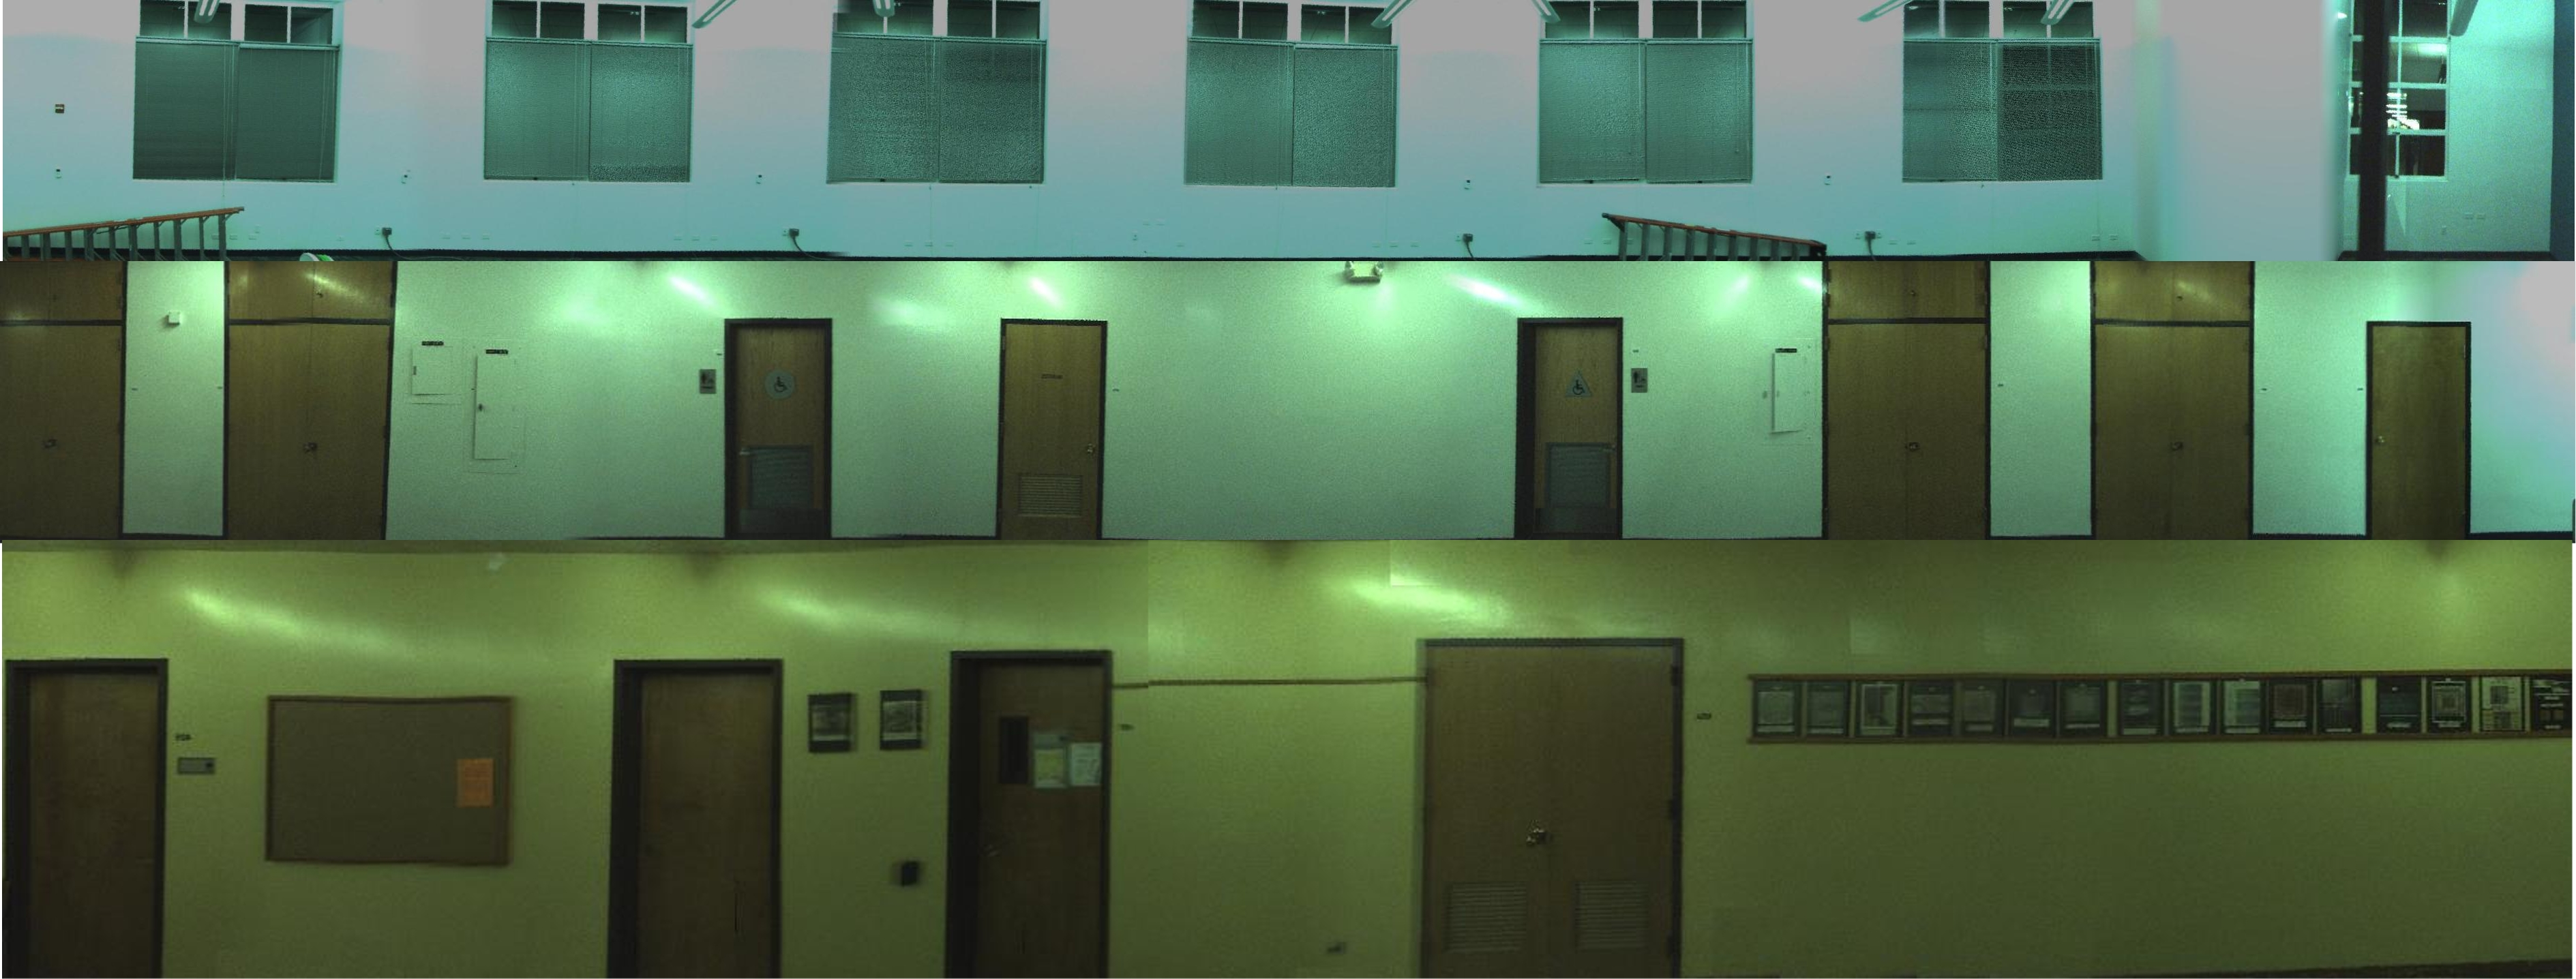
\includegraphics[width=6in]{finalfloors.jpg}} ~~~~~~~~
  \\
  \centering
  \subfloat[][]{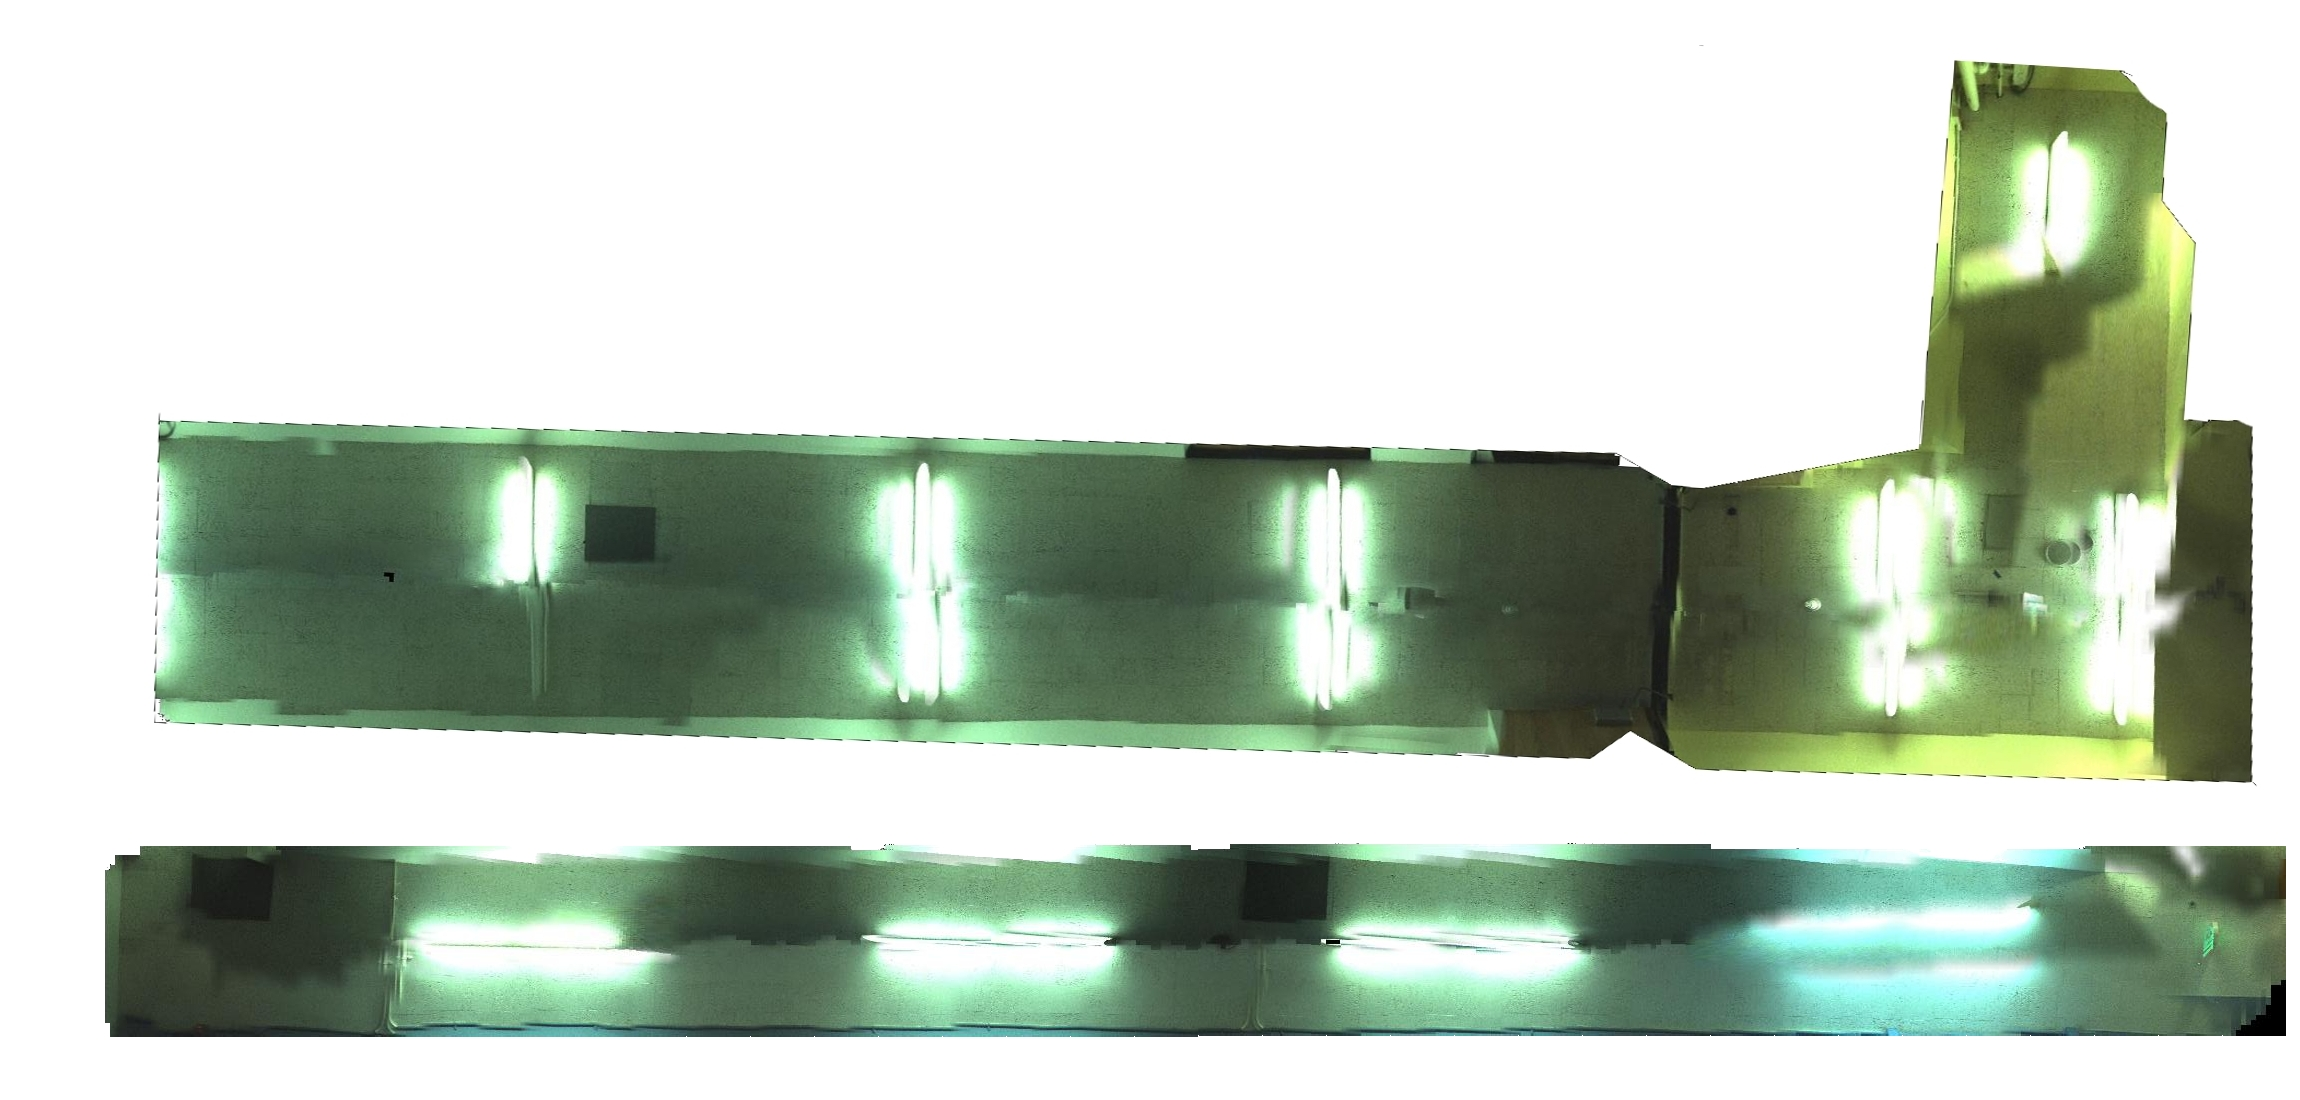
\includegraphics[width=6in]{finalceilings.jpg}}

  \centering \subfloat[][]{
    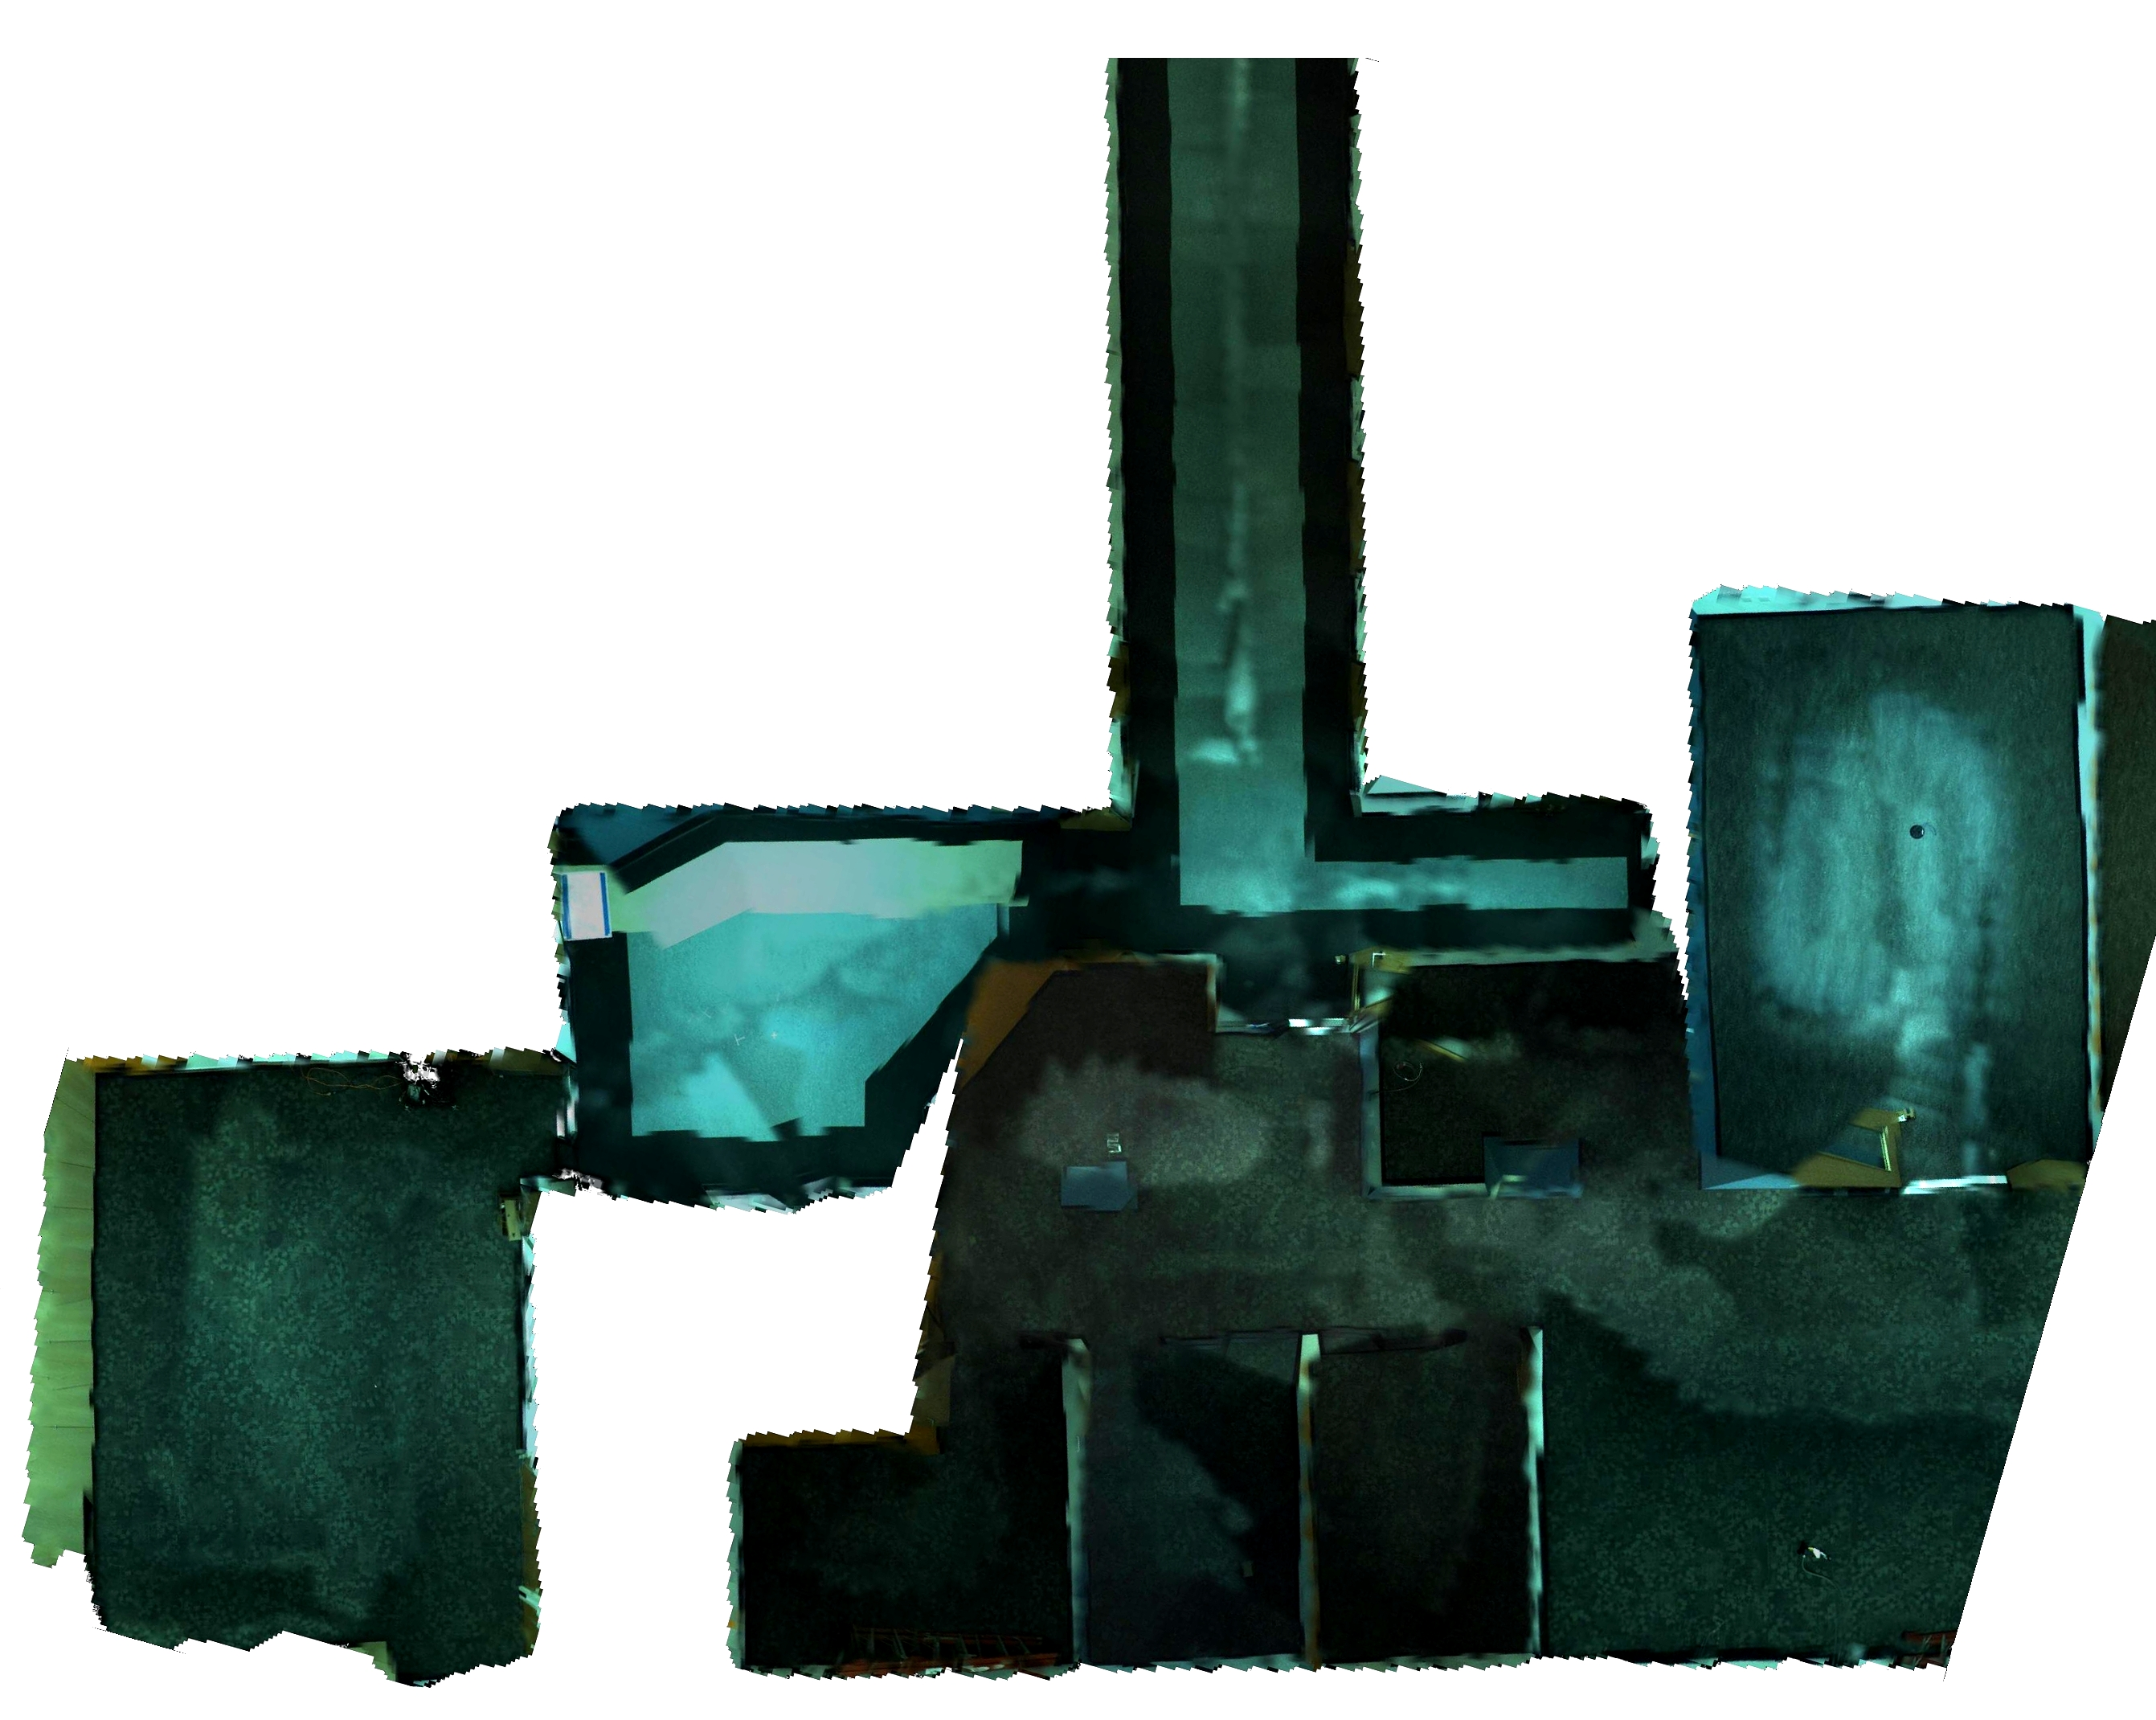
\includegraphics[height=2in, width=3in]{floorcropped.jpg} ~~~~~~~~
    \includegraphics[width=3in]{pier15floor.jpg}
  }
  \caption{Examples of our final texture mapping output for (a) walls,
    (b) ceilings, (c) floors}
  \label{fig:indivPlanes}
\end{figure}

\begin{figure}
  \centering{
    \includegraphics[width=6.2in]{threestoryfull2.png} \\
    \includegraphics[width=6.2in]{threestoryfull.png}
  }
  \caption{Textured low-resolution models from the PCA-based approach.}
  \label{fig:victor1}
\end{figure}

\begin{figure}
  \centering{
    \includegraphics[width=6.2in]{fullmodel.png} \\
    \includegraphics[width=6.2in]{pier15.png} \\
  }
  \caption{Textured low-resolution models from the PCA-based approach.}
  \label{fig:victor2}
\end{figure}

\begin{figure}
  \centering{
    \includegraphics[width=6.2in,height=3in]{houston2d1.png} \\
    \includegraphics[width=6.2in,height=3in]{houston2d2.png} \\
    \includegraphics[width=6.2in,height=3in]{houston3.png}
  }
  \caption{A textured low-resolution model from the floor plan extrusion approach.}
  \label{fig:e2d1}
\end{figure}

\begin{figure}
  \centering{
    \includegraphics[width=6.2in,height=3in]{coryf2.jpg} \\
    \includegraphics[width=6.2in,height=3in]{coryf2_2d_1.png} \\
    \includegraphics[width=6.2in,height=3in]{coryf2_2d_2.png}
  }
  \caption{A textured low-resolution model from the floor plan extrusion approach.}
  \label{fig:e2d2}
\end{figure}

\begin{figure}
  \centering{
    \includegraphics[width=6.2in,height=3in]{office.png} \\
    \includegraphics[width=6.2in,height=3in]{office1.png} \\
    \includegraphics[width=6.2in,height=3in]{office2.png}
  }
  \caption{A textured low-resolution model from the floor plan extrusion approach.}
  \label{fig:e2d3}
\end{figure}

\begin{figure}
  \centering{
    \includegraphics[width=6.2in,height=3in]{bhh1.png} \\
    \includegraphics[width=6.2in,height=3in]{bhh2.png} \\
    \includegraphics[width=6.2in,height=3in]{bhh3.png}
  }
  \caption{A textured low-resolution model from the floor plan extrusion approach.}
  \label{fig:e2d4}
\end{figure}





\begin{figure}
  \centering{
    \includegraphics[width=6.2in,height=3in]{houston1.jpg} \\
    \includegraphics[width=6.2in,height=3in]{houston2.jpg} \\
    \includegraphics[width=6.2in,height=3in]{houston3d2.png}
  }
  \caption{A textured high-resolution model from the voxel-carving approach.}
  \label{fig:e3d1}
\end{figure}
\begin{figure}
  \centering{
    \includegraphics[width=6.2in,height=3in]{coryf2_3d_4.png} \\
    \includegraphics[width=6.2in,height=3in]{coryf2_3d_2.png} \\
    \includegraphics[width=6.2in,height=3in]{coryf2_3d_3.png}
  }
  \caption{A textured high-resolution model from the voxel-carving approach.}
  \label{fig:e3d2}
\end{figure}
\begin{figure}
  \centering{
    \includegraphics[width=6.2in,height=3in]{bhh3d1.png} \\
    \includegraphics[width=6.2in,height=3in]{bhh3d2.png} \\
    \includegraphics[width=6.2in,height=3in]{bhh3d3.png}
  }
  \caption{A textured high-resolution model from the voxel-carving approach.}
  \label{fig:e3d3}
\end{figure}


%%%%%%%%%%%%%%%%%%%%%%%%%%%%%%%%%%%%%%%%%%%%%%%%%%%%%%%%%%%%%
%%%%% References %%%%%

\bibliography{report} %>>>> bibliography data in report.bib
\bibliographystyle{spiebib} %>>>> makes bibtex use spiebib.bst

\end{document} 
